\documentclass[a4paper,12pt,oneside,openany]{book}	
\usepackage{layout}
\setlength{\textwidth}{15.0 cm}
\setlength{\textheight}{25.0 cm}


\usepackage[english,brazil]{babel}
\usepackage{pagina}	% pagina-padrao
\usepackage{indentfirst}		% for indent
\usepackage[latin1]{inputenc}
\usepackage{graphics,epsfig}
\usepackage{graphics}
\graphicspath{{./figuras/}}
\usepackage{pstricks,pst-node,pst-tree}
\usepackage{alltt}
%\usepackage{makeidx}
%\makeindex
\usepackage[figuresright]{rotating} % for saydways tables and figures
\usepackage{enumerate}			% for configuration of enumerate environment
\usepackage{amsmath}
\usepackage{amssymb}
\usepackage{portland,multirow}

\usepackage{algorithm}
\usepackage[noend]{algpseudocode}

\usepackage{listings}
\usepackage{xcolor}

\usepackage[caption = false]{subfig}

% \usepackage[portuguese]{algorithm2e}

\setcounter{secnumdepth}{3}	% numeracao ate subsubsecao
\setcounter{tocdepth}{2}	% indice ate subsubsecao

\usepackage{longtable}


\begin{document}

\frontmatter
\thispagestyle{empty}


\includegraphics[scale=0.7]{Poli.eps}

\begin{center}
\large{MODELAGEM COMPUTACIONAL PARA ESTIMA��O DE CARACTER�STICAS DE ONDAS MAR�TIMAS EM BEIRA DE PRAIA}\\
   \vspace{2cm}
\large{David Estevam de Britto Junior}\\
\end{center}
   \vspace{3cm}
\hspace{7cm}
\hfill \parbox{8.0cm}{Projeto de Gradua��o apresentado ao Curso de Engenharia Eletr�nica e de Computa��o da Escola Polit�cnica, Universidade Federal do Rio de Janeiro, como parte dos requisitos necess�rios � obten��o do t�tulo de Engenheiro.\\}
   \vspace{2cm}
\hfill \parbox{8.0cm}{Orientador: Fl�vio Luis de Mello} \\
   \vspace{2cm}
\begin{center}
Rio de Janeiro

Agosto de 2017
\end{center}




\pagebreak

% \input{figuras/folha_assinatura_banca.pdf}

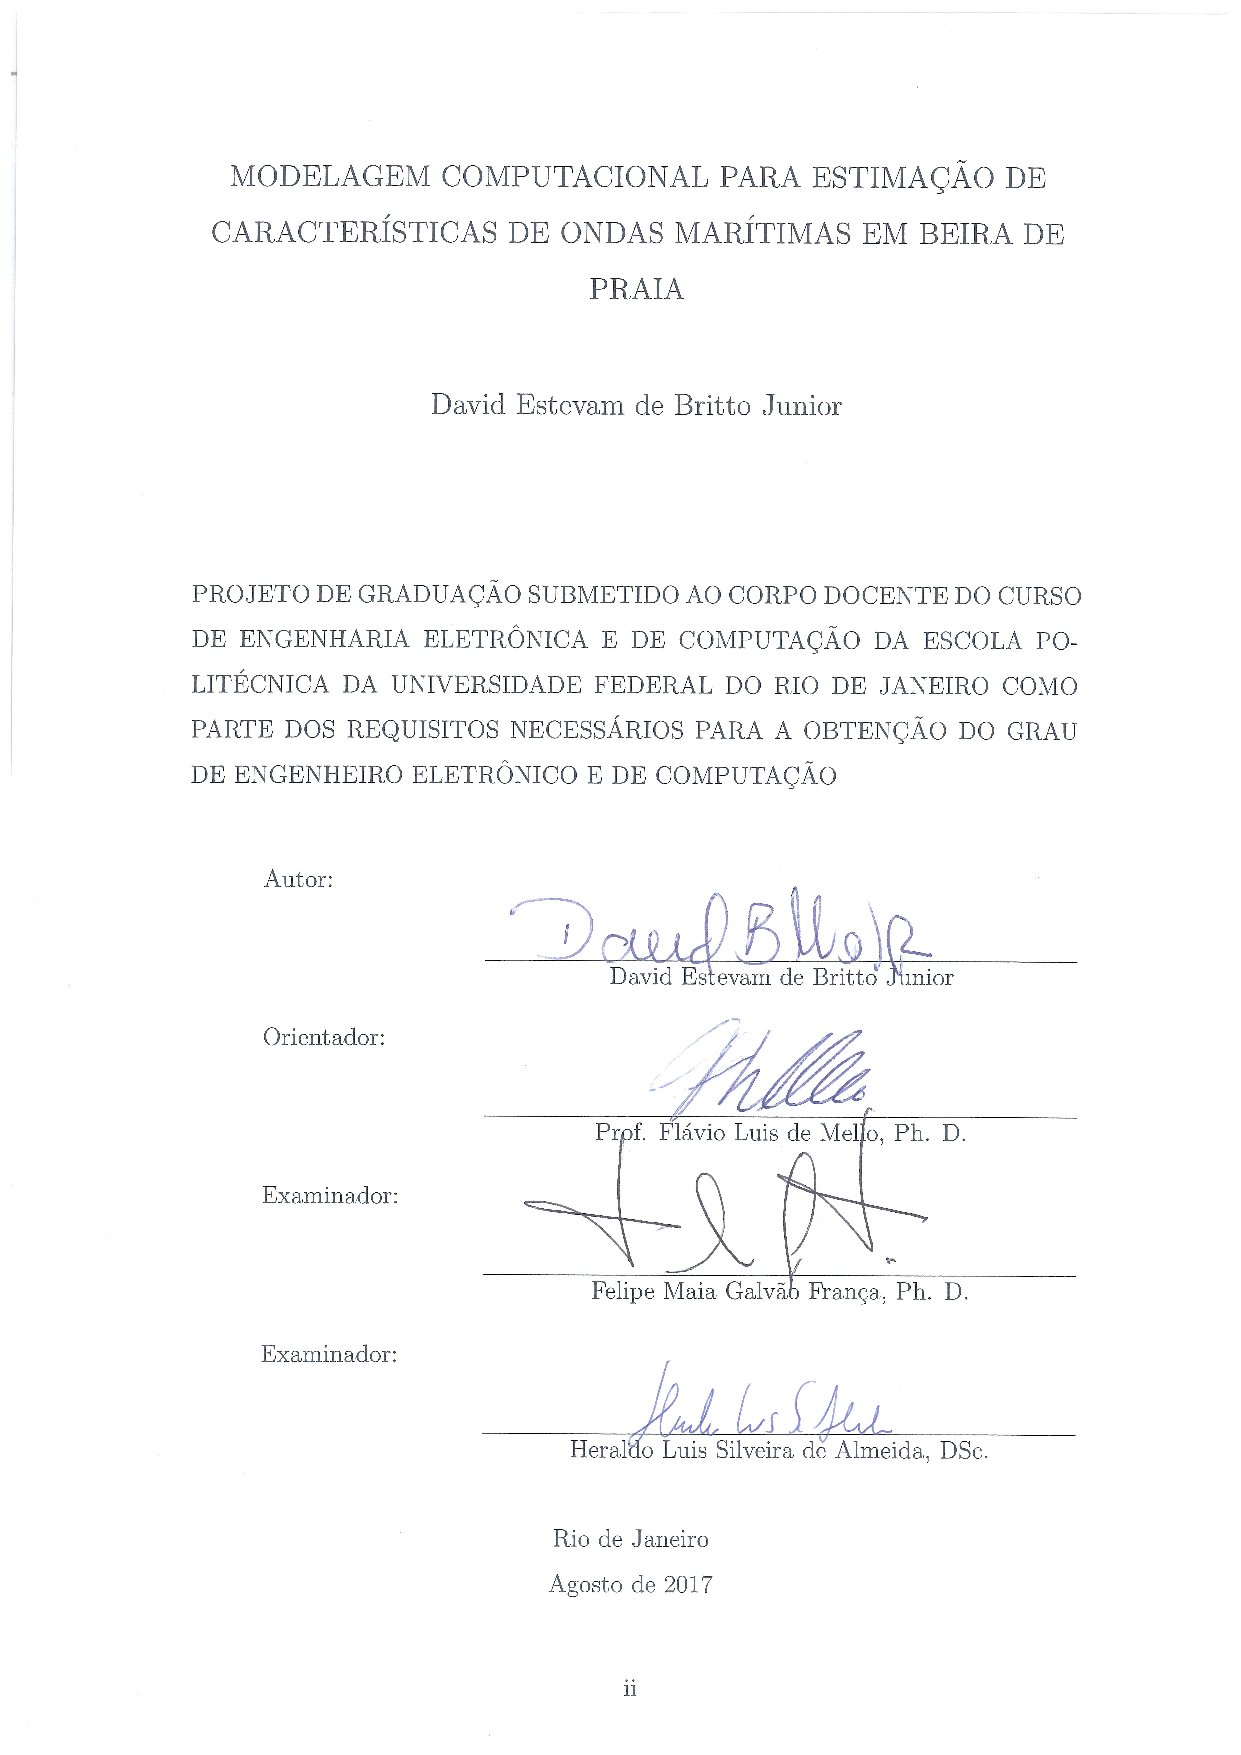
\includepdf{folha_assinatura_banca.pdf}

% \begin{figure}
%    \centering
%    \includefigure
% \end{figure}

% \begin{center}
% \large{MODELAGEM COMPUTACIONAL PARA ESTIMA��O DE CARACTER�STICAS DE ONDAS MAR�TIMAS EM BEIRA DE PRAIA}\\
%    \vspace{1cm}
% \large{David Estevam de Britto Junior}\\
% \end{center}
%    \vspace{2cm}
% PROJETO DE GRADUA��O SUBMETIDO AO CORPO DOCENTE DO CURSO DE ENGENHARIA ELETR�NICA E DE COMPUTA��O DA ESCOLA POLIT�CNICA DA UNIVERSIDADE FEDERAL DO RIO DE JANEIRO COMO PARTE DOS REQUISITOS NECESS�RIOS PARA A OBTEN��O DO GRAU DE ENGENHEIRO ELETR�NICO E DE COMPUTA��O   
   
%    \vspace{1cm}
% Autor:
%       \vspace{0.5cm}
%       \begin{flushright}
%          \parbox{10cm}{
%             \hrulefill

%             \vspace{-.375cm}
%             \centering{David Estevam de Britto Junior}

%             \vspace{0.1cm}
%          }
%       \end{flushright}
      
      
% Orientador:
%       \vspace{0.5cm}
%       \begin{flushright}
%          \parbox{10cm}{
%             \hrulefill

%             \vspace{-.375cm}
%             \centering{Prof. Fl\'avio Luis de Mello, Ph. D.}

%             \vspace{0.1cm}
%          }
%       \end{flushright}
      
% Examinador:
%       \vspace{0.5cm}
%       \begin{flushright}
%          \parbox{10cm}{
%             \hrulefill

%             \vspace{-.375cm}
%             \centering{Felipe Maia Galv�o Fran�a, Ph. D.}

%             \vspace{0.1cm}
%          }
%       \end{flushright}
      
% Examinador:
%       \vspace{0.5cm}
%       \begin{flushright}
%          \parbox{10cm}{
%             \hrulefill

%             \vspace{-.375cm}
%             \centering{Heraldo Luis Silveira de Almeida, DSc.}

%             \vspace{0.1cm}
%          }
%       \end{flushright}
      
                        
%       \vfill
      
      
% \begin{center}
% Rio de Janeiro

% Agosto de 2017
% \end{center}


\pagebreak            

% Declaracao
\begin{center}
Declara��o de Autoria e de Direitos
\end{center}

\vspace{0.5cm}

Eu, \emph{David Estevam de Britto Junior} CPF \emph{137.221.577-81}, autor da monografia \emph{Modelagem Computacional para Estima��o de Caracter�sticas de Ondas Mar�timas em Beira de Praia}, subscrevo para os devidos fins, as seguintes informa��es:\\
1. O autor declara que o trabalho apresentado na disciplina de Projeto de Gradua��o da Escola Polit�cnica da UFRJ � de sua autoria, sendo original em forma e conte�do.\\
2. Excetuam-se do item 1. eventuais transcri��es de texto, figuras, tabelas, conceitos e id�ias, que identifiquem claramente a fonte original, explicitando as autoriza��es obtidas dos respectivos propriet�rios, quando necess�rias.\\
3. O autor permite que a UFRJ, por um prazo indeterminado, efetue em qualquer m�dia de divulga��o, a publica��o do trabalho acad�mico em sua totalidade, ou em parte. Essa autoriza��o n�o envolve �nus de qualquer natureza � UFRJ, ou aos seus representantes.\\
4. O autor pode, excepcionalmente, encaminhar � Comiss�o de Projeto de Gradua��o, a n�o divulga��o do material, por um prazo m�ximo de 01 (um) ano, improrrog�vel, a contar da data de defesa, desde que o pedido seja justificado, e solicitado antecipadamente, por escrito, � Congrega��o da Escola Polit�cnica.\\
5. O autor declara, ainda, ter a capacidade jur�dica para a pr�tica do presente ato, assim como ter conhecimento do teor da presente Declara��o, estando ciente das san��es e puni��es legais, no que tange a c�pia parcial, ou total, de obra intelectual, o que se configura como viola��o do direito autoral previsto no C�digo Penal Brasileiro no art.184 e art.299, bem como na Lei 9.610.\\
6. O autor � o �nico respons�vel pelo conte�do apresentado nos trabalhos acad�micos publicados, n�o cabendo � UFRJ, aos seus representantes,  ou ao(s) orientador(es), qualquer responsabiliza��o/ indeniza��o nesse sentido.\\
7. Por ser verdade, firmo a presente declara��o.\\

      \vspace{0.5cm}
      \begin{flushright}
         \parbox{10cm}{
            \hrulefill

            \vspace{-.375cm}
            \centering{David Estevam de Britto Junior}

            \vspace{0.1cm}
         }
      \end{flushright}
      
\pagebreak

% Copyright
      \vspace{0.5cm}

UNIVERSIDADE FEDERAL DO RIO DE JANEIRO \\
Escola Polit�cnica - Departamento de Eletr�nica e de Computa��o \\
Centro de Tecnologia, bloco H, sala H-217, Cidade Universit�ria \\ 
Rio de Janeiro - RJ      CEP 21949-900\\
\vspace{0.5cm}
\paragraph{}Este exemplar � de propriedade da Universidade Federal do Rio de Janeiro, que poder� inclu�-lo em base de dados, armazenar em computador, microfilmar ou adotar qualquer forma de arquivamento.
\paragraph{}� permitida a men��o, reprodu��o parcial ou integral e a transmiss�o entre bibliotecas deste trabalho, sem modifica��o de seu texto, em qualquer meio que esteja ou venha a ser fixado, para pesquisa acad�mica, coment�rios e cita��es, desde que sem finalidade comercial e que seja feita a refer�ncia bibliogr�fica completa.
\paragraph{}Os conceitos expressos neste trabalho s�o de responsabilidade do(s) autor(es).


\pagebreak

% Dedicat�ria
\begin{center}
\textbf{DEDICAT�RIA}
\end{center}
      \vspace{0.5cm}

\paragraph{}Opcional.

\pagebreak


% Agradecimento
\begin{center}
\textbf{AGRADECIMENTO}
\end{center}
      \vspace{0.5cm}

\paragraph{}Sempre haver�. Se n�o estiver inspirado, aqui est� uma sugest�o: dedico este trabalho ao povo brasileiro que contribuiu de forma significativa � minha forma��o e estada nesta Universidade. Este projeto � uma pequena forma de retribuir o investimento e confian�a em mim depositados.

\pagebreak


% Resumo
\begin{center}
\textbf{RESUMO}
\end{center}
      \vspace{0.5cm}

\paragraph{}Inserir o resumo do seu trabalho aqui. O objetivo � apresentar ao pretenso leitor do seu Projeto Final uma descri��o gen�rica do seu trabalho. Voc� tamb�m deve tentar despertar no leitor o interesse pelo conte�do deste documento.
\paragraph{}
\noindent Palavras-Chave: trabalho, resumo, interesse, projeto final.

\pagebreak


% Abstract
\begin{center}
\textbf{ABSTRACT}
\end{center}
      \vspace{0.5cm}

\paragraph{}Insert your abstract here. Insert your abstract here. Insert your abstract here. Insert your abstract here. Insert your abstract here.
\paragraph{}
\noindent Key-words: word, word, word.

\pagebreak


% Siglas
\begin{center}
\textbf{SIGLAS}
\end{center}
      \vspace{0.5cm}

\paragraph{}UFRJ - Universidade Federal do Rio de Janeiro 
\paragraph{}WYSIWYG - \textit{What you see is what you get} 


\pagebreak









% Table of Contents
% ---------------------------------------------------------------
     \tableofcontents
% ---------------------------------------------------------------
% Lista de figuras
% ---------------------------------------------------------------
%\cleardoublepage
%\addcontentsline{toc}{chapter}{Lista de Figuras}
\listoffigures
% ---------------------------------------------------------------
% Lista de Tabelas
% ---------------------------------------------------------------
%\cleardoublepage
%\addcontentsline{toc}{chapter}{Lista de Tabelas}
\listoftables

\mainmatter
\cleardoublepage
% ---------------------------------------------------------------
% Chapter 1 - Introdu��o
% ---------------------------------------------------------------
\chapter{Introdu��o}
\label{cap1}
\section{Tema}

\paragraph{}O tema deste trabalho � o uso de intelig�ncia de m�quina e vis�o computacional para estimar dados sobre ondas em uma cabe�a de praia. Neste sentido, o problema a ser resolvido � construir uma solu��o de hardware e software capaz de inferir a altura de ondas e sua periodicidade.

\section{Delimita��o}

\paragraph{}Esse estudo ser� realizado com base em ondas na praia de Itacoatiara, Niter�i. Os dados foram coletados inicialmente utilizando uma c�mera de celular, e posteriormente utilizando um aparato de hardware desenvolvido para o projeto. A captura de dados usando um dispositivo m�vel introduz algumas dificuldades no projeto, como instabilidades nos v�deos capturados. Entretanto, utilizar um hardware em um local fixo apresenta outros problemas, como produzir um hardware que aguente exposi��o ao tempo e encontrar um local seguro para fix�-lo.



\section{Justificativa}

\paragraph{}Hoje, os m�todos mais difundidos para medi��o de ondas do mar s�o: m�todo gr�fico e m�todo sensorial. O m�todo gr�fico � utilizado principalmente em campeonatos de surf, onde o tamanho do surfista � usado como refer�ncia para calcular a altura da onda. J� o m�todo sensorial utiliza boias com sensores de movimento, instaladas em um ponto na praia, de forma que a passagem das ondas altera a altura do sensor de movimento, e com isso pode-se calcular a diferen�a da altura inicial para a final.

\paragraph{}Ambos os m�todos descritos anteriormente n�o s�o pr�ticos de serem implementados em larga escala. O m�todo gr�fico necessita sempre de uma refer�ncia para realizar a medi��o de cada onda, al�m de necessitar o ajuste humano em cada medida. O m�todo sensorial � custoso para adquirir, instalar e manter o equipamento necess�rio.

\paragraph{}Uma das caracter�sticas desejadas para esse sistema de monitoramento � que ele deveria ser aut�nomo e distribu�do, podendo monitorar diversas praias em tempo real. Logo de in�cio ficou claro que medir a altura das ondas de uma forma automatizada e barata � essencial para o sistema, e ainda, que todos os m�todos existentes n�o atendem esses requisitos.

\paragraph{}Inicialmente, este projeto come�ou como parte de um sistema de monitoramento de praias voltado para avalia��o da condi��o de surf, chamado GoSurf. O sistema foi desenvolvido na disciplina Projeto Integrado. Entretanto, no desenvolvimento inicial do sistema n�o foi poss�vel implementar uma forma de medi��o de ondas do mar satisfat�rio.

\paragraph{}O monitoramento de praias possui outras aplica��es fora do sistema descrito anteriormente. Um sistema similar, tamb�m baseado em imagens, foi desenvolvido na Griffin University, Australia, para indicar n�vel de perigo para nado em praias e que ser� objeto de estudo na fundamenta��o te�rica deste trabalho \cite{Griffith05}.

\paragraph{}O estudo de processamento de imagens voltado a ondas do mar apresenta um problema interessante em an�lise de imagens. Como se est� trabalhando com imagens reais e altamente din�micas, deve-se empregar diversas t�cnicas para reduzir o ru�do nos dados de entrada e garantir uma medi��o confi�vel.

\paragraph{}Assim, torna-se desej�vel criar e implementar um algoritmo para medir a altura de ondas do mar utilizando t�cnicas de processamento de imagens. A an�lise de cen�rios naturais din�micos � um desafio na �rea de an�lise de imagens, uma vez que n�o se pode alterar o cen�rio para facilitar a an�lise desejada. Por isso � necess�rio um algoritmo inteligente que consiga se adaptar a varia��es nos dados de entrada para extrair as informa��es relevantes.



\section{Objetivos}

\paragraph{}Informar qual � o objetivo geral do trabalho, isto �, aquilo que deve ser atendido e que corresponde ao indicador inequ�voco do sucesso do seu trabalho. Pode acontecer que venha a existir um conjunto de objetivos espec�ficos, que complementam o objetivo geral (tamanho do texto: livre, mas cuidado para n�o fazer uma literatura romanceada, afinal esta se��o trata dos objetivos).
\begin{itemize}
\item Construir um aparato de aquisi��o de v�deos  montado em uma praia. 
\item Adquirir os v�deos e transmiti-los para um servidor.
\item Realizar medi��es (este item pode ser fragmentado em outras metas)
\item Disponibilizar os dados. 
\end{itemize}

\section{Metodologia}

\paragraph{}As medi��es obtidas pelo algoritmo ser�o comparadas com medi��es manuais tanto nas imagens geradas quanto por estimativas in loco. As medi��es manuais s�o feitas na imagem por um operador humano. Inspecionando a imagem, � f�cil perceber onde � o ponto de m�ximo e m�nimo de uma onda, e com o aux�lio de um programa de edi��o de imagem pode-se contar o n�mero de pixels entre esses dois pontos. As medi��es in loco s�o realizadas no mesmo momento que as imagens s�o obtidas. Como n�o � poss�vel medir a onda atrav�s de instrumentos, vale-se da experi�ncia da pessoa realizando a aquisi��o dos dados e de outras no local para estimar a altura das ondas naquele momento. Essa estimativa serve para validar se o processo de calcular dimens�es reais baseadas nas dimens�es em pixels est� na ordem de grandeza correta.

\paragraph{}Para certificar a confiabilidade do algoritmo, ser�o avaliados in�meros dados de uma mesma praia, contemplando varia��es de clima, ilumina��o, angula��o e posicionamento da c�mera, mar� e ocupa��o da praia. Todos esses fatores podem interferir com o resultado do algoritmo, principalmente as mudan�as de mar� e posicionamento da c�mera. A escolha de uma posi��o para a c�mera adequada � fundamental para minimizar o efeito dos outros fatores no resultado final.


\section{Descri��o}

\paragraph{}No cap�tulo 2 ser� .....

\paragraph{}O cap�tulo 3 apresenta ...

\paragraph{}Os .... s�o apresentados no cap�tulo 4. Nele ser� explicitado ...

\paragraph{}E assim vai at� chegar na conclus�o.


% ---------------------------------------------------------------
% Chapter 2 - Embasamento Te�rico
% ---------------------------------------------------------------
\chapter{Fundamenta��o Te�rica}
\label{cap2}
\section{Trabalhos Relacionados}

\paragraph{}A an�lise de praias e mares atrav�s de imagens n�o � algo novo. O uso de c�meras oferece uma grande vantagem em rela��o a outros tipos de sensores, como descrito por Holland\cite{Holland97}, "T�cnicas de v�deo s�o particularmente atraentes na documenta��o de processos oceanogr�ficos pr�ximos a costa uma vez que a localiza��o suba�rea do instrumento (distante da superf�cie do oceano) alivia algumas das dificuldades associadas com instrumenta��o \textit{in situ}, como a perturba��o de correntes, bioincrusta��o e deteriora��o dos sensores em condi��es adversas de ondas". Entretanto, n�o existem muitos projetos diretamente ligados � an�lise de ondas mar�timas utilizando processamento de imagem. O desenvolvimento mais not�rio nessa �rea � feito na Griffith University, Austr�lia, onde foram desenvolvidos alguns projetos e t�cnicas de monitoramento de praias que ser�o descritos a seguir. 

%Griffith05
\paragraph{}Browne \textit{et al.} \cite{Griffith05} descrevem um sistema inteligente que monitora e prediz as condi��es de uma praia para banho. O objetivo desse sistema �, em caso de perigo, alertar aos banhistas e �s autoridades sobre o estado da praia em tempo real. O sistema obt�m dados da praia de duas fontes: de c�meras posicionadas \textit{in loco} e de servidores do \textit{Bureau of Meteorology} australiano.
As imagens obtidas s�o pr�-processadas, extraindo dados como tamanho e frequ�ncia das ondas e a localiza��o da arrebenta��o. Dos servidores s�o obtidos dados em tempo real sobre as mar�s, vento e \textit{swell}, que s�o as ondas formadas por tempestades e ventos distantes, e n�o por vento local. Uma vez obtidos os dados, o sistema alimenta uma rede neural treinada que determina se a praia � segura para banho.

%Griffith10
\paragraph{}Outro sistema estudado � chamado de \textit{WavePack} \cite{Griffith10}, descrito nesse artigo apenas de forma n�o-t�cnica. Esse sistema tem como objetivo apenas medir a altura, frequ�ncia e localiza��o do momento que uma onda quebra, utilizando c�meras montadas em pontos baixos, dez metros acima da praia. O sistema � descrito em quatro etapas: obten��o das imagens, convers�o do \textit{stream} de v�deo em \textit{timestack}, an�lise do \textit{timestack}, apresenta��o dos resultados. O artigo ainda compara os resultados obtidos com outras fontes de dados de ondas mar�timas, e comprova que o sistema produz dados confi�veis. 

%Griffith11 e Griffith14
\paragraph{}O algoritmo implementado no sistema \textit{WavePack} � descrito em um artigo \cite{Griffith11} posterior. Esse artigo descreve o m�todo de: 1) identificar a arrebenta��o, e 2) identificar cada onda individual na arrebenta��o e calcular a sua altura em \textit{pixels}, filtrando a perturba��o de objetos indesejados na imagem (como barcos e pessoas). Em seguida, � discutida e apresentada a rela��o entre a altura de uma onda medida em \textit{pixels} e a sua altura no mundo real, em metros. Por �ltimo, apresenta-se os resultados obtidos, novamente comparados com outros m�todos j� existentes. Esse m�todo � tamb�m apresentado tamb�m � apresentado em um artigo \cite{Griffith14} mais recente. Esse artigo descreve com maiores detalhes o pr�-processamento que ocorre no \textit{timestack}, e a rela��o entre a altura da onda encontrada em \textit{pixels} e a altura em metros no mundo real.

\paragraph{}Essas pesquisas serviram de grande inspira��o para o desenvolvimento deste projeto, mostrando que ele � fact�vel. Os resultados desses projetos servir�o como par�metro de valida��o dos aqui resultados encontrados.

\paragraph{}No Brasil n�o � conhecido algum sistema de monitoramento de praias automatizado. No Rio de Janeiro o site RicoSurf\cite{Rico17} prov�m um monitoramento manual de algumas praias locais e de cidades pr�ximas, se expandindo at� Guarapari, ES. O monitoramento � feito atrav�s de boletins dispon�veis no site, que normalmente s�o feitos uma ou duas vezes ao dia por uma pessoa que vai at� a praia e reporta a condi��o encontrada. Este m�todo � pouco pr�tico se aplicado em grande escala, � subjetivo e demanda uma quantidade cada vez maior de rep�rteres para analisar cada praia. 

\section{Processamento de V�deo e Imagens}

\paragraph{}Processamento de Imagem � uma sequ�ncia de opera��es realizadas em uma ou mais imagens de entrada, resultado em uma imagem de sa�da ou caracter�sticas extra�das das imagens de entrada. Uma imagem, conforme definido por Rafael Gonzalez \cite{Gonzalez92} �: "[...] uma fun��o bidimensional \(f(x,y)\), onde \(x\) e \(y\) s�o coordenadas espaciais (plano), e a amplitude de \(f\) de qualquer par de coordenadas \((x,y)\) � chamada de intensidade ou n�vel de cinza da imagem naquele ponto.".

\paragraph{}Neste projeto, como em outras aplica��es de oceanografia \cite{Jahne02} \cite{Holland97}, imagens est�ticas do objeto de estudo s�o pouco produtivas para extrair informa��es. Por isso, uma solu��o encontrada foi capturar e trabalhar com um v�deo da arrebenta��o de uma praia, ao inv�s de usar apenas fotografias. 

\paragraph{}Um v�deo � definido como uma sequ�ncia temporal de imagens. De forma an�loga a imagem, um v�deo pode ser descrito como uma fun��o tridimensional \(g(x,y,t)\), onde \(x\) e \(y\) s�o coordenadas espaciais, como em uma imagem, e \(t\) � uma coordenada temporal. A amplitude \(g\) � a intensidade ou n�vel de cinza do ponto \((x,y)\) no instante de tempo \(t\).

\paragraph{}A principal vantagem de utilizar um v�deo � eliminar o problema de identificar qual � o melhor momento para analisar a onda fotografada. Utilizando uma sequ�ncia de imagens, � mais f�cil de determinar qual foi o momento em que a onda estava maior, e ai sim realizar a medi��o de sua altura. Ser� demonstrado adiante que o \textit{timestack} tamb�m ajuda a tornar as imagens analisadas mais uniformes, criando regi�es bem definidas para segmenta��o. 



\section{Identifica��o de objetos}

\paragraph{}Para extrair os dados desejados de uma imagem, � necess�rio separar o que � o objeto de estudo -- no caso espec�fico deste projeto, uma onda do mar -- do restante da imagem. Isto �, atrav�s de transforma��es na imagem original deseja-se identificar o que � o primeiro plano e o plano de fundo. Este processo de extra��o de objetos ou planos de uma imagem � chamado na literatura de segmenta��o \cite{Gonzalez92}.

\paragraph{}Antes de aplicar as t�cnicas de segmenta��o, precisa-se melhorar a imagem. O processo de aprimoramento de imagens, segundo Rafael Gonzalez \cite{Gonzalez92}, � fundamental para torn�-la adequada para a aplica��o desejada. O aprimoramento permite real�ar alguma caracter�stica de interesse da imagem, enquanto minimiza a presen�a de outras caracter�sticas n�o relevantes.

\paragraph{}Os m�todos de aprimoramento de imagens podem ser estudados em dois dom�nios: dom�nio espacial e dom�nio da frequ�ncia. O aprimoramento no dom�nio espacial trabalha com os pr�prios \textit{pixels} de uma imagem, e podem ser representados pela express�o: \(g(x,y) = T[f(x,y)]\), onde \( g(x,y) \) � a imagem transformada, \( f(x,y) \) � a imagem original e \( T[ \ \cdot\  ] \) � a transforma��o que ser� aplicada na imagem original. As t�cnicas de aprimoramento no dom�nimo da frequ�ncia procuram implementar um filtro que possui uma resposta em frequ�ncia espec�fica para realizar a opera��o desejada, que podem ser representadas pela express�o: $G(j\Omega) = H(j\Omega)F(j\Omega)$, onde $F(j\Omega)$ � a imagem original representada no dom�nio da frequ�ncia, $H(j\Omega)$ � a resposta em frequ�ncia do filtro que ser� aplicado e $G(j\Omega)$ � a imagem resultante desta opera��o. Em algumas aplica��es, trabalhar no dom�nio da frequ�ncia ser� vantajoso, e em outras ser� vantajoso trabalhar no dom�nio espacial. � importante lembra que os m�todos no dom�nio espacial e no dom�nio da frequ�ncia s�o equivalentes. Neste cap�tulo todos os m�todos ser�o apresentados no dom�nio espacial.

\paragraph{}Alguns m�todos de aprimoramento de imagens ser�o utilizados nesse projeto: transforma��es em n�veis de cinza, filtros de nitidez (\textit{sharpening}), filtros de suaviza��o (\textit{blur}), filtros de detec��o de bordas. Esses m�todos s�o importantes para melhorar o contraste entre as regi�es da imagem analisada e reduzir o ru�do, facilitando assim o processo de segmenta��o que ser� realizado posteriormente.

\paragraph{}As transforma��es em n�veis de cinza englobam m�todos que alteram o contraste de uma imagem. Em geral, s�o m�todos onde cada pixel \((x,y)\) da sa�da depende apenas do pixel correspondente da entrada, ou seja, n�o � influenciado pelos seus vizinhos. O principal m�todo que ser� utilizado nesse projeto � o de \textit{thresholding}, onde a transforma��o aplicada na entrada � da forma: 

\[
T[f(x,y)] =
\begin{cases}
	f(x,y), & \text{se } f(x,y) > C\\
	0, & \text{se } f(x,y) < C
\end{cases}
\] 

\noindent{}Onde C � uma constante escolhida arbitrariamente. A utilidade dessa fun��o � facilitar a defini��o das regi�es da imagem, quais fazem parte do c�u, do mar e da arrebenta��o.

\paragraph{}Os filtros de suaviza��o, tamb�m conhecidos como filtros de \textit{blur} s�o importantes para reduzir o n�vel de ru�do na imagem. Outra fun��o importante para esse projeto � homogeneizar as regi�es da imagem, isto �, eliminar, ou pelo menos reduzir, pontos mais claros em regi�es escuras, ou pontos escuros em regi�es claros. Dessa forma, os m�todos de \textit{thresholding} s�o mais efetivos.

\paragraph{}Neste projeto o filtro de suaviza��o utilizado � o filtro passa-baixas gaussiano. Este filtro, como definido em \cite{Gonzalez92}, possui a seguinte forma:

\[
H(u,v) = e^{-D^{2}(u,v)/2D^{2}_{0}}
\]

\noindent{}\(D(u,v)\) � definido como a dist�ncia da origem da transformada de Fourier, e \(D^{2}_{0}\) � definido como \(\sigma^{2}\), ou a vari�ncia da curva gaussiana.

\paragraph{}Segundo Bernd J�hne \cite{Jahne02}, um filtro de suaviza��o deve atender algumas propriedades especificas para ser aplic�vel a identifica��o de objetos e extra��o de dados de uma imagem. As propriedades s�o:

\begin{enumerate}

\item Desvio de fase zero, isto �, o filtro n�o deve causar desvio na fase da imagem a fim de n�o alterar a posi��o dos objetos na mesma.

\item Preserva��o da m�dia, isto �, a soma de todos os fatores da m�scara no dom�nio espacial deve ser igual a 1.

\item Monotonicidade, isto �, a fun��o de transfer�ncia do filtro de suaviza��o deve decrescer monotonicamente.

\item Equidade, isto �, a fun��o de transfer�ncia deve ser isotr�pica, a fim de n�o privilegiar nenhuma dire��o na imagem.

\end{enumerate}




\paragraph{}No in�cio do projeto foram pesquisados e utilizados m�todos de nitidez, ou \textit{sharpening}. A fun��o desses m�todos � aumentar o contraste da imagem na fronteira de regi�es, isto �, onde ocorre uma descontinuidade de \textit{pixels}. O m�todo utilizado neste projeto � o m�todo Laplaciano. Segundo Gonzalez \cite{Gonzalez92}, o Laplaciano de uma imagem \(f(x,y)\) � definido por:

\[
	\nabla^{2}f = \frac{\partial^{2}f}{\partial x^{2}} + \frac{\partial^{2}f}{\partial y^{2}}
\]

\paragraph{}As derivadas parciais da equa��o acima podem ser escritas na forma discreta:

\[
	\frac{\partial^{2}f}{\partial x^{2}} = f(x + 1,y) + f(x - 1,y) - 2f(x,y)
\]

\noindent{}e

\[
	\frac{\partial^{2}f}{\partial y^{2}} = f(x,y + 1) + f(x,y - 1) - 2f(x,y)
\]

\noindent{}\newline{}Dessa forma, o Laplaciano bidimensional discreto � dado por:

\[ 
	\nabla^{2}f = f(x + 1,y) + f(x - 1,y) + f(x,y + 1) + f(x,y - 1) - 4f(x,y) 
\]

\paragraph{}A aplica��o de um operador Laplaciano em uma imagem resulta em suas apenas as suas descontinuidades. Pela defini��o do Laplaciano discreto, � f�cil perceber que regi�es com valores intensidades pr�ximas se anulam, resultado em um Laplaciano pr�ximo de zero, enquanto regi�es com descontinuidade a diferen�a de intensidade se refor�a. Para recuperar as regi�es anuladas pelo Laplaciano e enfim aplicar o efeito de \textit{sharpening} na imagem, basta somar o resultado do Laplaciano com a imagem original:

\[ 
	g(x,y) = f(x,y) + \nabla^{2}f(x,y) 
\] 

\noindent{}Onde \(g(x,y)\) � a imagem de sa�da e \(f(x,y)\) � a imagem de entrada. Entretanto, a medida que o projeto progrediu percebeu-se que o refor�o na intensidade das bordas realizado pelos m�todo de \textit{sharpening} n�o compensavam o aumento de ru�do introduzido na imagem, portanto foram descartados do projeto.




\paragraph{}Por �ltimo, utiliza-se um m�todo para normalizar a luminosidade da imagem, de forma que seja poss�vel processar tanto dias de alta luminosidade (c�u sem nuvens e sol forte) quanto dias de baixa luminosidade (c�u nublado e sol fraco). Esta normaliza��o pode ser realizada atrav�s da equaliza��o do histograma da imagem. Gonzalez \cite{Gonzalez92} define um histograma de uma imagem digital com 0 at� L-1 n�veis de cinza como uma fun��o discreta $h(r_ {k}) = n_{k}$, onde $r_{k}$ � o k-�simo n�vel de cinza e $n_{k}$ � o n�mero de \textit{pixels} com o n�vel de cinza $r_{k}$. Esta fun��o pode ser normalizada pelo n�mero total de \textit{pixels} $n$, a fun��o normalizada $p(r_{k})$ � definida como:

\[
	p(r_{k}) = \frac{n_{k}}{n}
\]

\noindent{}A fun��o $p(r_{k})$ pode ser interpretada como a probabilidade da ocorr�ncia do n�vel de cinza $r_{k}$ na imagem digital. A equaliza��o do histograma consiste em encontrar uma transforma��o T que quando aplicada no histograma normalizado $p(r_{k})$ que resulta em um histograma uniforme. Gonzalez demonstra que a seguinte transforma��o atinge este objetivo:

\[
	s_{k} = T(r_{k}) = \sum_{j=0}^{k} \frac{n_{j}}{n}
\]

\noindent{}Onde $k = 0,1,2,...,L-1$ e $s_{k}$ � a fun��o que representa o histograma equalizado. 



\section{M�todos de Segmenta��o de Imagens}

\paragraph{}Segmenta��o � definido como um processo que, a partir de uma imagem de entrada, a subdivide em objetos ou nas suas regi�es constituintes. O n�vel de subdivis�es que ser�o obtidas depende de cada aplica��o, e segundo Gonzalez: "A segmenta��o deve parar quando os objetos de interesse em uma aplica��o estejam isolados" \cite{Gonzalez92}. Al�m diso, Gonzalez continua: "A segmenta��o de imagens n�o-triviais � uma das tarefas mais dif�ceis em processamento de imagem" \cite{Gonzalez92}.

\paragraph{}O primeiro passo para realizar a segmenta��o � aplicar um m�todo de detec��o de bordas. O m�todo escolhido para esse projeto � o m�todo de Canny \cite{Canny86}, que � hoje o m�todo mais eficaz de detec��o de bordas \cite{Juneja09}. Esse m�todo basea-se em criar um modelo matem�tico para uma borda e definir tr�s restri��es que o modelo deve atender, e ent�o utilizar um m�todo num�rico para otimizar o modelo. As restri��es definidas por Canny \cite{Canny86} s�o:

\begin{enumerate}

\item Boa detec��o. Deve haver uma baixa probabilidade de detectar bordas inexistentes ou n�o detectar bordas existentes.

\item Boa localiza��o. A localiza��o das bordas detectadas deve estar pr�xima da localiza��o das bordas reais.

\item Resposta �nica para cada borda. Uma borda n�o pode ser detectada multiplas vezes.

\end{enumerate}

\noindent{}Outro m�todo de detec��o de bordas considerado foi o m�todo de Sobel \cite{Gonzalez92}, que � utilizado em \cite{Griffith11} para evidenciar bordas verticais. Uma diferen�a importante entre os dois m�todo � que o m�todo de Sobel atua em cada dire��o separadamente, podendo-se somar o resultado de cada dire��o para obter uma resposta unificada, enquanto o m�todo de Canny atua em todas as dire��es simultaneamente. Devido a maior presen�a de ru�do nas imagens capturadas, o m�todo de Canny mostrou-se mais eficaz em eliminar o ru�do e detectar apenas as bordas desejadas.

\paragraph{}O segundo passo do processo de segmenta��o � aplicar um m�todo de extra��o de regi�es. Inicialmente o m�todo de watershed \cite{Gonzalez92} foi considerado para tal tarefa. O algoritmo de watershed baseia-se na id�ia de enxergar a imagem em tr�s dimens�es como um vales que ser�o "inundados", sendo \(x\) e \(y\) coordenadas espaciais e a intensidade de cada pixel \(g(x,y)\) a "altura" de cada ponto neste vale. Os pontos de m�nimo locais, ou seja, os pontos onde \(g(x,y)\) � m�nimo localmente, consideramos este um ponto mais baixo de um vale, e a regi�o ao redor que ser� segmentada sua zona de influ�ncia. A partir dos pontos de m�nimo locais inunda-se a imagem, preenchendo-a com valores gradativamente maiores de intensidade de pixel em sua zona de influ�ncia, como seria o n�vel de �gua subindo em uma inunda��o. Eventualmente, a inunda��o da zona de influ�ncia de um ponto m�nimo local ir� "vazar" para a zona de influ�ncia de outro ponto m�nimo local. Quando isso ocorre, constr�i-se uma "barragem" com largura de um pixel entre as duas zonas de influ�ncia, para evitar o vazamento. Quando o n�vel de inunda��o atinge o ponto m�ximo da imagem, isto �, o valor m�ximo de \(g(x,y)\), o algoritmo de watershed � interrompido. As regi�es segmentadas ser�o definidas pelas "barragens" formadas durante a execu��o do algoritmo. Na forma descrita acima, o algoritmo de watershed pode levar a segmenta��o de mais regi�es que se desejava originalmente. Isso � corrigido atrav�s do uso de marcadores, indicadores de quais s�o os pontos de m�nimo local que ser�o utilizados pelo algoritmo.

\paragraph{}No decorrer do projeto o m�todo de watershed foi preterido em prol do m�todo de Suzuki \cite{Suzuki85}, um m�todo de rastreamento e hierarquiza��o de bordas em imagens bin�rias. O m�todo de Suzuki realiza um rastreamento de linha na imagem, procurando por pixels com intensidade diferente de zero. Quando um \textit{pixel} que atende a esta condi��o � encontrado, � atribuindo um valor para ele, e se rastreia todos os outros \textit{pixels} conectados a ele. Uma vez que toda a borda � detectada, o algoritmo continua o rastreamento na regi�o interna, atribu�ndo para estes \textit{pixels} internos valores maiores que os externos. Este processo se repete at� que n�o existam mais pixels internos. O algoritmo � interrompido quando o rastreamento de linha atinge uma das extremidades inferior da imagem, sinalizando que toda a imagem foi rastreada. O resultado deste algoritmo � um conjunto de bordas hierarquizadas. O cap�tulo 3 apresentar� como este m�todo pode ser utilizado para identificar uma regi�o desejada, atingindo o mesmo resultado desejado do m�todo de watershed.

\section{Modelo Geom�trico de C�meras}
\label{sec:camera}

\paragraph{}Todos os m�todos descritos anteriormente foram apresentados com o intuito de aplic�-los no c�lculo da altura de uma onda em pixels. Para obter a altura em metros, precisa-se de um modelo matem�tico que relacione as duas medidas. O modelo mais simples de uma c�mera � o modelo furo-de-agulha. Segundo Fusiello \cite{Fusiello}, o modelo � descrito pelo seu centro �tico \(C\) e o plano da imagem. A dist�ncia entre \(C\) e o centro do plano da imagem, � chamado de dist�ncia focal \(f\). O eixo perpendicular ao plano da imagem que passa pelo centro �tico � chamado de eixo principal.

\begin{figure}[h]
\begin{center}
  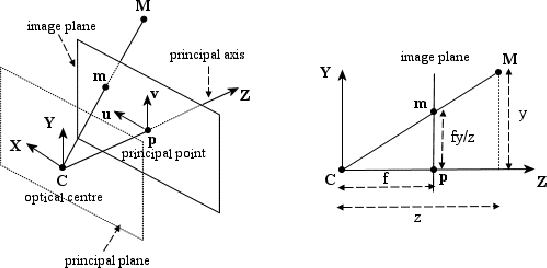
\includegraphics[scale=0.7]{pin_hole_camera.png}
  \caption[\small{Modelo de C�mera Furo-de-Agulha. Fonte: School of Informatics/University of Edinburgh \cite{Fusiello}.}]{\label{FigFusiello} \small{Modelo de C�mera Furo-de-Agulha. Fonte: School of Informatics/University of Edinburgh \cite{Fusiello}.}}
\end{center}
\end{figure}

\noindent{}Este modelo apresenta uma forma simples de calcular a rela��o entre a altura aparente de um objeto em uma imagem e a sua altura real, dependendo apenas da dist�ncia focal da c�mera e da dist�ncia real do objeto. Esta rela��o �:

\[
	h_{real} = z * h_{aparente} / f
\]

\noindent{}onde \(z\) � a dist�ncia real do objeto, \(f\) � a dist�ncia focal, \(h_{real}\) e \(h_{aparente}\) s�o, respectivamente, a altura real e a altura aparente.

\section{Modelo Geom�trico de Uma Praia}

\paragraph{}Browne \textit{et al.} \cite{Griffith14} descreve um modelo geom�trico simplificado de uma praia, onde temos uma rela��o direta entre a altura em pixels de uma onda e a sua altura real. Para isso, s�o necess�rios tr�s par�metros de montagem da c�mera: o �ngulo da c�mera em rela��o ao ponto de montagem (\(\phi_{t}\)), o �ngulo de \textit{zoom} da c�mera (\(\phi_{z}\)) e a altura da c�mera em rela��o ao n�vel do mar (\(h_{c}\)).

\begin{figure}[h]
\begin{center}
  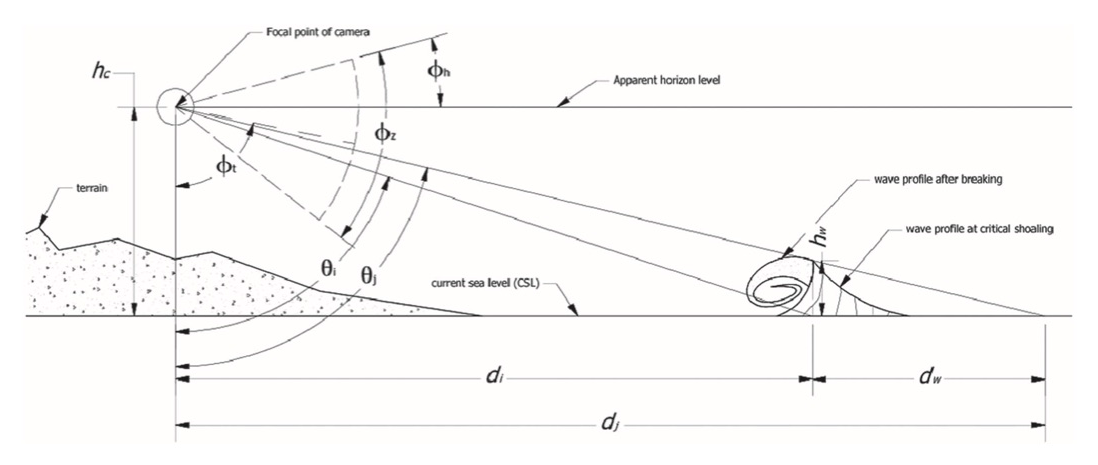
\includegraphics[scale=0.8]{beach_model_griffith.png}
  \caption[\small{Modelo Geom�trico de uma Praia e C�mera. Fonte: Griffith University \cite{Griffith14}.}]{\label{FigBeachModel} \small{Modelo Geom�trico de uma Praia e C�mera. Fonte: Griffith University \cite{Griffith14}.}}
\end{center}
\end{figure}

\paragraph{}A altura real de uma onda na imagem pode ser calculada pela equa��o:

\[
	h_{w} = h_{c}\Bigg(1 - \frac{tan(\theta_{i})}{tan(\theta_{j})}\Bigg)
\]

\noindent{}Onde \(h_{w}\) � a altura real de uma onda, \(\theta_{i}\) � o �ngulo calculado do ponto mais baixo de uma onda e \(\theta_{j}\) � o ponto mais alto de uma onda. Utilizando uma c�mera com baixa distor��o, � poss�vel calcular o �ngulo \(\theta_{k}\) de um pixel \((x,k)\) atrav�s da equa��o:

\[
	\theta_{k} = \phi_{t} - \frac{\phi_{z}}{2} + \frac{k\phi_{z}}{V}
\]
\noindent{}onde \(V\) � a altura da imagem em pixels. A vantagem deste modelo em rela��o ao modelo furo-de-agulha � ser n�o s� mais preciso, mas n�o depender da dist�ncia da c�mera at� a onda (valor $z$ do Modelo de C�mera Furo-de-Agulha), que pode ser altamente vari�vel.



% ---------------------------------------------------------------
% Chapter 3 - Algoritmo de Medi��o de Altura das Ondas do Mar
% ---------------------------------------------------------------
\chapter{Algoritmo de Medi��o de Altura das Ondas do Mar}
\label{cap3}
\newcommand{\timestack}[0]{\textit{timestack} }
\newcommand{\threshold}[0]{\textit{threshold} }

\paragraph{}Os m�todos apresentados no Cap�tulo 2 agora ser�o utilizadas em conjunto para estimar a altura de ondas do mar. Este algoritmo � composto de tr�s etapas: o pr�-processamento, o processamento principal, e a an�lise da imagem resultante. Estas etapas ser�o detalhadas nas se��es a seguir.

\section{Pr�-Processamento}

\begin{figure}[h]
  \subfloat[\textit{Pipeline} do pr�-processamento.]{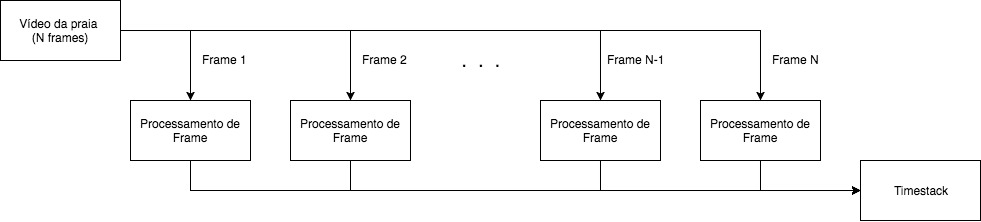
\includegraphics[width=\textwidth,keepaspectratio]{pre_processamento_pipeline.png}}
  \qquad
  \subfloat[Processamento de cada \textit{frame}.]{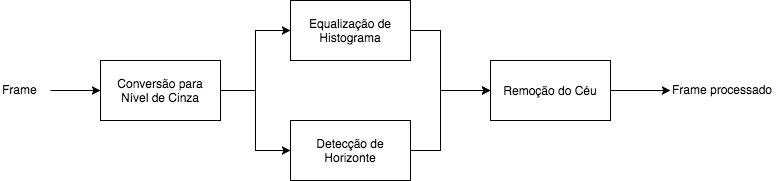
\includegraphics[width=\textwidth,keepaspectratio]{pre_processamento_frame.png}}
  \caption[\small{Diagrama de Bloco da etapa de pr�-processamento.}]{\small{Diagrama de Bloco da etapa de pr�-processamento.}}
  \label{FigDiagramaPreProc}
\end{figure}

\paragraph{}A etapa de pr�-processamento tem como objetivo transformar os dados de entrada (o v�deo capturado de uma praia) em uma imagem \timestack  pronta para ser processada e analisada pelos passos subsequentes. O pr�-processamento atua sobre cada \textit{frame} do v�deo, realizando as seguintes opera��es: convers�o para n�vel de cinza, equaliza��o de histograma, detec��o da linha de horizonte, remo��o do c�u. Ap�s operar cada \textit{frame} do v�deo � gerado um \timestack das imagens processadas. A figura \ref{FigDiagramaPreProc} ilustra os passos realizados.

\paragraph{}O passo mais importante nessa etapa � a cria��o do \timestack, que � uma representa��o espa�o-temporal de um v�deo. O \timestack � a imagem que ser� processada pelo processamento principal e analisada para extra��o dos dados das ondas do mar. Os demais passos servir�o para garantir a confiabilidade do \timestack e o preparar�o para a etapa de processamento principal.

\paragraph{}O pr�-processamento inicia a partir do v�deo capturado de uma praia. Cada \textit{frame} do v�deo � processado, primeiro convertendo o \textit{frame} para uma imagem em n�veis de cinza, pois todos os processamentos posteriores s� operam sobre o n�vel de intensidade de cada \textit{pixel}. A seguir, equaliza-se o histograma do \textit{frame}, a fim de normalizar a ilumina��o da imagem. Esta opera��o � necess�ria para possibilitar que filmagens realizadas em qualquer hora do dia podem ser tratadas da mesma forma. Os passos seguintes s�o a detec��o da linha do horizonte e a remo��o do c�u. Para detectar o horizonte, analisa-se o \frame original em n�vel de cinza. Uma vez detectada a linha do horizonte, o c�u � removido simplesmente alterando todos \textit{pixels} acima da linha para intensidade zero. O �ltimo passo � gerar o \timestack a partir dos \textit{frames} do v�deo. O \timestack � gerado selecionando a coluna central de cada \textit{frame}, acumulando-as sequencialmente em uma �nica imagem. Todos esses passos ser�o descritos detalhadamente a seguir.

\section{\textit{Timestack}}

\paragraph{}Um \timestack � uma representa��o bidimensional de um v�deo, isto �, trata-se de uma forma de transformar tal v�deo em uma s� imagem. O \timestack � �til para analisar tais v�deos pois � poss�vel olhar para uma sequ�ncia completa de quadros observando uma �nica imagem. Dessa forma, pode-se aplicar m�todos de processamento de uma �nica imagem \timestack, em vez de todo o v�deo.

\paragraph{}Para construir um \timestack, � necess�rio fixar uma das dimens�es espaciais de cada imagem do v�deo, obtendo assim um conjunto de fun��es unidimensionais. O \timestack deste v�deo � definido ent�o como uma fun��o bidimensional \(s_{Y}(x,t)\) ou \(s_{X}(t,y)\), onde \(x\) e \(y\) s�o coordenadas espaciais; \(t\) � uma coordenada temporal; as amplitudes \(s_{X}\) e \(s_{Y}\) s�o a intensidade ou n�vel de cinza do v�deo \(g(x,y,t)\) quando s�o fixados os valores \(x = X\) e \(y = Y\), respectivamente. Dessa forma, a rela��o entre um \timestack e um v�deo � dada por: \(s_{Y}(x,t)=g(x,Y,t)\) e \(s_{X}(t,y) = g(X,y,t)\).

\begin{figure}[h]
  \centering
  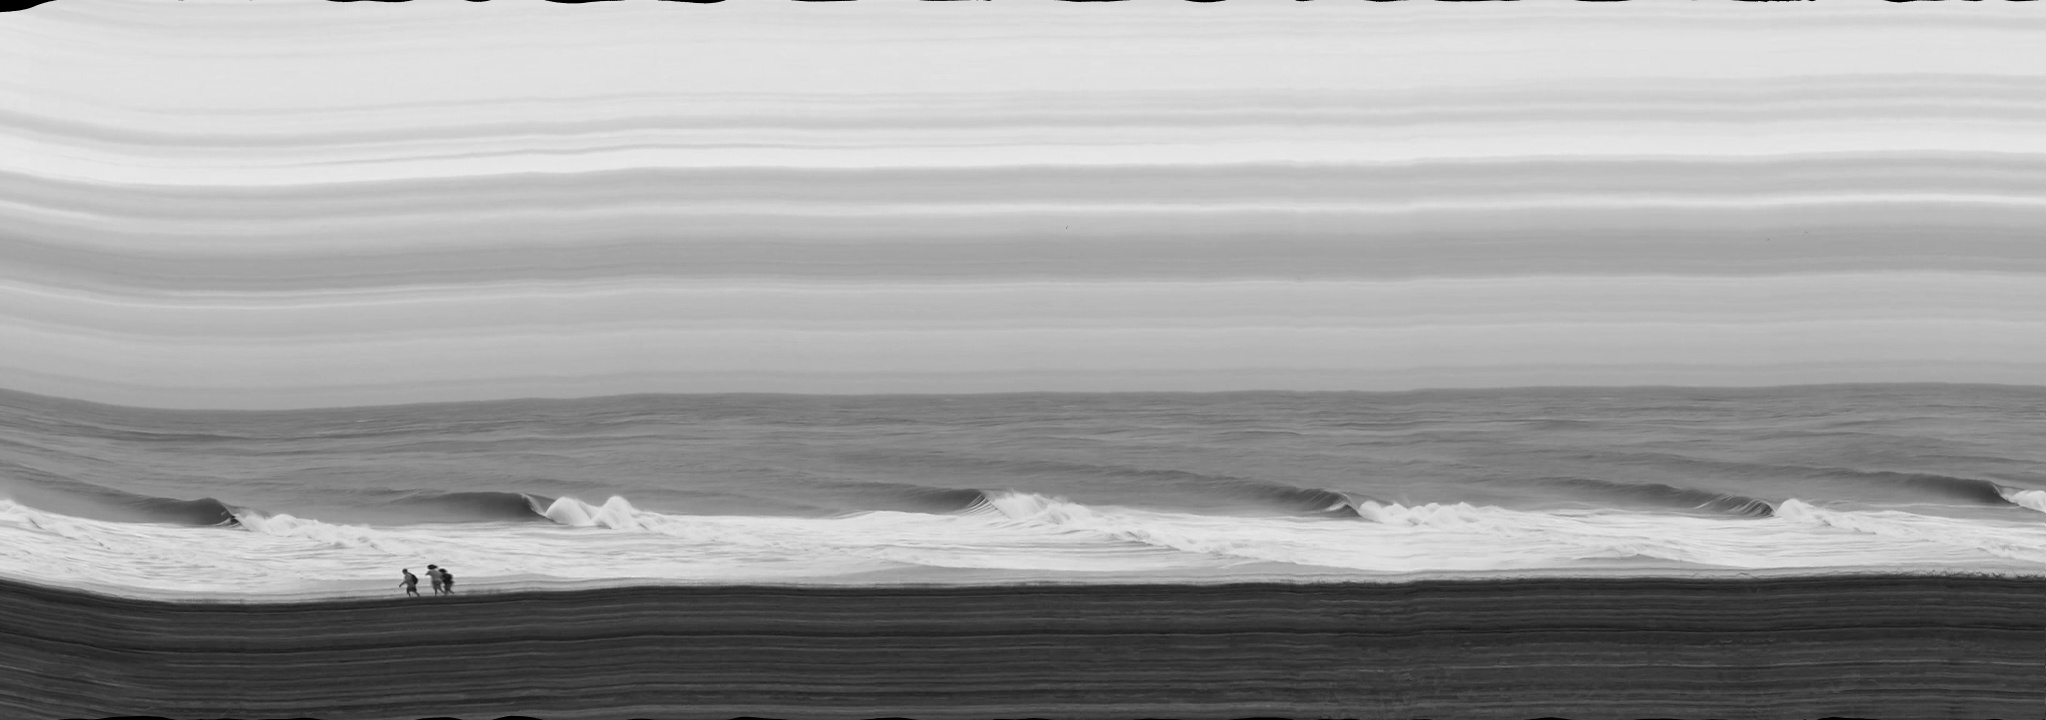
\includegraphics[width=\textwidth,keepaspectratio]{timestack.jpg}
  \caption[\small{\textit{Timestack} resultante do pr�-processamento a partir do v�deo de uma praia.}]{\small{\textit{Timestack} resultante do pr�-processamento a partir do v�deo de uma praia.}}
  \label{FigTimestack}
\end{figure}

\paragraph{}Note que, na pr�tica, a coordenada temporal \(t\) cumpre o papel de uma coordenada espacial quando o \timestack � exibido como uma imagem, mas sua interpreta��o continua sendo temporal. Como � poss�vel notar na figura \ref{FigTimestack}, cada onda aparenta crescer a medida que se desloca da esquerda para a direita e de cima para baixo. Isso ocorre pois o deslocamento horizontal representa a evolu��o temporal da onda, representa eventos que est�o ocorrendo sequencialmente, primeiro a onda cresce at� que chega no seu ponto m�ximo e quebra. O deslocamento vertical representa o avan�o da onda at� quebrar na areia da praia.

\paragraph{}� importante lembrar que a perda de uma dimens�o resulta em perda de informa��o no v�deo, entretanto, nos casos em que o v�deo se mant�m constante na dimens�o espacial fixada n�o h� perda de informa��o. Expandindo esse conceito, nos casos em que o v�deo varie muito pouco em uma de suas dimens�es espaciais, n�o h� necessariamente uma perda de conte�do significativa.

\paragraph{}A an�lise de ondas mar�timas apresenta condi��o similar a descrita anteriormente. Com a posi��o da c�mera escolhida com cuidado, isto �, a zona de arrebenta��o deve centralizada na imagem, tanto horizontalmente quando verticalmente. A c�mera deve estar perpendicular em rela��o a zona de arrebenta��o, e montada em um ponto acima do n�vel da praia, de forma que banhistas na areia n�o atrapalhem a vis�o da zona de arrebenta��o. Assim, uma onda quebrando ocupar� maior parte horizontal da imagem. Al�m disso, n�o � importante para a an�lise desejada entender o tamanho horizontal da onda, apenas o seu tamanho vertical. Precisa-se apenas determinar o seu ponto mais baixo e seu ponto mais alto. Sendo assim, o \timestack mostra-se um m�todo adequado de an�lise de v�deos para esse projeto.

\section{Aparato Instrumental}

% Est� esquecendo do seu trabalho de projeto integrado. Trazer ele para c� fazendo refer�ncia aos seus colegas co-autores.

\paragraph{}Como mencionado anteriormente este projeto foi concebido como parte do sistema de monitoramento de praias \textit{GoSurf}, sendo o monitoramento por imagens apenas uma parte do sistema. Esse sistema foi criado para a disciplina Projeto Integrado no ano letivo 2015.1, em conjunto com outro aluno, Filipe Barretto. Para este fim foi desenvolvido um aparato instrumental que adquire dos dados e os analisa previamente por meio de uma central de processamento de dados, e por fim os envia para um servidor na nuvem. O servidor finaliza o processamento dos dados e disponibiliza para os resultados para os usu�rios por um aplicativo \textit{Android}.

\paragraph{}No projeto de gradua��o as imagens foram adquiridas de duas formas: atrav�s de c�meras de \textit{smartphones} comuns e atrav�s da c�mera montada no \textit{hardware} apresentado anteriormente. Embora para este projeto a c�mera de \textit{smartphones} atenda o requisito, o aparato instrumental � fundamental para o projeto \textit{GoSurf} completo porque agrega sensores extra al�m da c�mera. Outra vantagem do aparato sensorial � a capacidade de realizar o pr�-processamento localmente, o que reduz drasticamente o volume de dados que devem ser enviado ao servidor. Por exemplo, um v�deo de 125MB � reduzido para uma imagem de 657KB.

\paragraph{}A central de processamento utilizada no projeto GoSurf e no projeto de gradua��o � um Raspberry Pi, um pequeno computador implementado em uma �nica placa. O Raspberry Pi � um computador completo, sendo poss�vel instalar diversos sistemas operacionais diferentes. Neste projeto seguiu-se a recomenda��o oficial e foi utilizado o sistema operacional Raspbian - um sistema operacional Linux baseado em Debian. Por ser baseado em Linux, pode-se utilizar a biblioteca OpenCV para agilizar a implementa��o do projeto de gradua��o.

\paragraph{}Um dos motivos para a escolha do Raspberry Pi foi a facilidade de integrar com uma c�mera. Existe um m�dulo de c�mera oficial para o Raspberry Pi \ref{RaspberryCamera}, que foi a c�mera escolhida para este projeto. Utilizando este m�dulo e o sistema operacional Raspbian, a integra��o com o projeto � trivial, basta conectar a c�mera � central de processamento. Esta c�mera � capaz de capturar v�deos com resolu��o 1080p a 30 \textit{frames} por segundo, a mesma qualidade de v�deo utilizada em capturas de v�deo com \textit{smartphones}. O m�dulo de c�mera possui ponto focal fixo na faixa de 1 metro at� o infinito, o que n�o � um problema para o algoritmo pois os objetos de estudo, as ondas do mar, est�o localizados nesta faixa. O campo de vis�o vertical desta c�mera � de 41.41 graus (mais ou menos 0.11 graus). Este dado ser� importante durante a convers�o da altura das ondas estimada em \textit{pixels} para metros.

\paragraph{}O Raspberry Pi ainda conta com um conjunto de pinos de entrada e sa�da de uso gen�rico (\textit{GPIOs}). Uma desvantagem do Raspberry Pi com rela��o a outras centrais de processamento � que ele n�o possu� \textit{GPIOs} anal�gicos, somente pinos digitais. Entretanto, como ser� comentado a seguir, � poss�vel contornar esta desvantagem utilizando conversores anal�gico-digitais. Estes pinos foram utilizados para ligar os sensores perif�ricos no projeto GoSurf, um term�metro/higr�metro e um anem�metro. Um circuito simples (Figura \ref{FigPCB}) foi projetado para ligar os sensores � central de processamento. O term�metro / higr�metro utilizado foi o DHT22, que pode ser lido diretamente por um pino digital. Por este motivo ele pode ser ligado diretamente aos pinos da central de processamento, acrescentando somente um resistor \textit{pullup} de 1k$\Omega$ entre sua alimenta��o e o pino de leitura. O anem�metro escolhido foi o C2192, que possu� um pino de leitura anal�gico. Para utiliz�-lo com o Raspberry Pi foi necess�rio adicionar um conversor anal�gico-digital (MCP 3201). Este conversor foi escolhido por apresentar resolu��o adequada ao projeto (12 \textit{bits}) e possuir interface de sa�da SPI (\textit{Serial Peripheral Interface} ou Interface Perif�rica Serial). O Raspberry Pi implementa uma comunica��o SPI em pinos espec�ficos, o que torna f�cil integrar os dois componentes. Por fim, foi necess�rio adicionar uma alimenta��o externa ao circuito, pois o anem�metro precisa de uma alimenta��o de 7 a 12 volts e a central de processamento s� � capaz de fornecer 5V. Foram adicionados um par de pilhas de 4.5V, resultando em uma alimenta��o total de 9V que atende ao requisito. 

\begin{figure}[h]
  \centering
  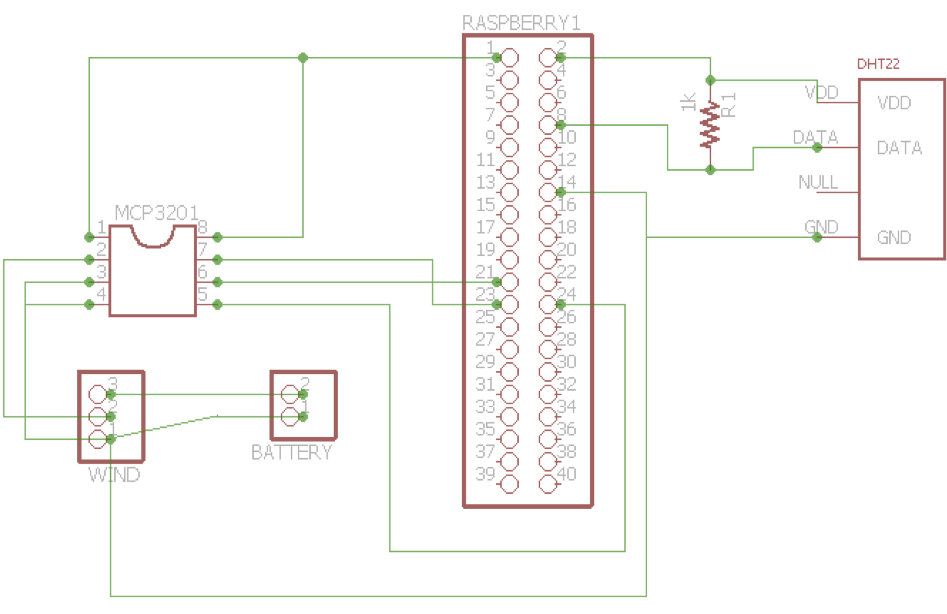
\includegraphics[width=.8\textwidth,keepaspectratio]{pcb.png}
  \caption[\small{Circuito que conecta os sensores � central de processamento.}]{\small{Circuito que conecta os sensores � central de processamento.}}
  \label{FigPCB}
\end{figure}
%Observe que a inten��o desta se��o de aparato instrumental � mostrar o hardware utilizado. Aqui voc� apenas mencionou que existe um hardware. Descreva aqui o hardware do seu experimento.

\section{Estabiliza��o de V�deo}

\paragraph{}A estabiliza��o do v�deo � fundamental para a cria��o de um \timestack fiel ao cen�rio real. Esta necessidade surge uma vez que o \timestack � criado selecionando a coluna central de cada \textit{frame} do v�deo, tornando importante que esta coluna corresponda ao mesmo conjunto de \textit{pixels} de quadro a quadro. Caso a c�mera se desloque horizontalmente no decorrer do v�deo, o conjunto de \textit{pixels} n�o ser� o mesmo, e com isso o \timestack formado n�o ser� uma representa��o fiel em duas dimens�es do v�deo capturado. A estabilidade na dire��o vertical � importante para que a estimativa de altura das ondas seja fiel a altura real. Um deslocamento vertical da c�mera resulta em um deslocamento das colunas do \timestack, que por sua vez podem embutir erros na identifica��o dos pontos de m�ximo e m�nimo de cada onda.

\paragraph{}Primeiro experimentou-se realizar a estabiliza��o do v�deo utilizando t�cnicas de processamento de imagens. Foi testado um procedimento simples descrito por Nghia Ho \cite{Ho2014}. Embora este procedimento apresente bons resultados para v�deos gravados manualmente (figura \ref{FigStabilization}a e \ref{FigStabilization}b), foi observado que quando aplicado o procedimento em v�deos gravados j� com alta estabilidade o procedimento n�o apresentava resultados significativos (Figura \ref{FigStabilization}c e \ref{FigStabilization}d). Entretanto, o processo de estabiliza��o � custoso, aumentando o tempo de execu��o do pr�-processamento (na figura \ref{FigStabilization} o tempo de execu��o do pr�-processamento foi 8.5 vezes maior.). Como o pr�-processamento ser� executado em um dispositivo com poder de processamento limitado, a performance desta etapa � crucial. Ent�o, concluiu-se que basta utilizar um ponto de montagem para a c�mera, como um trip�, para atingir a estabilidade necess�ria para a extra��o fiel dos dados desejados.

\begin{figure}[h]
  \centering
  \subfloat[\small{\textit{Timestack} gerado a partir de um v�deo gravado manualmente.}]{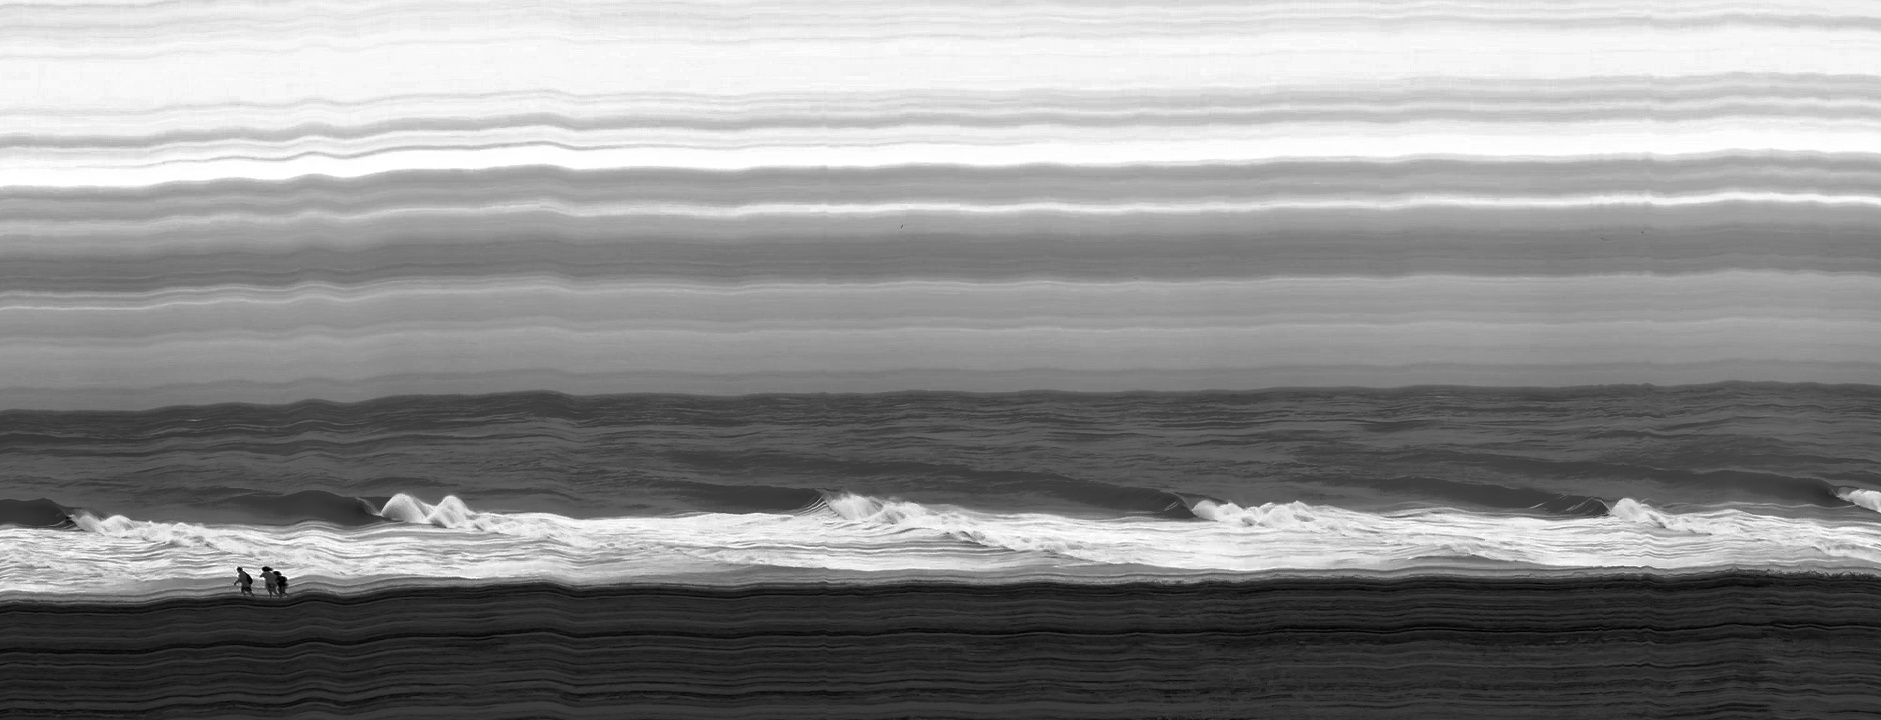
\includegraphics[width=.45\textwidth,keepaspectratio]{IMG_0798_2_originalTimestack.jpg}}
  \qquad
  \subfloat[\small{\textit{Timestack} gerado a partir de um v�deo gravado manualmente e estabilizado por \textit{software}.}]{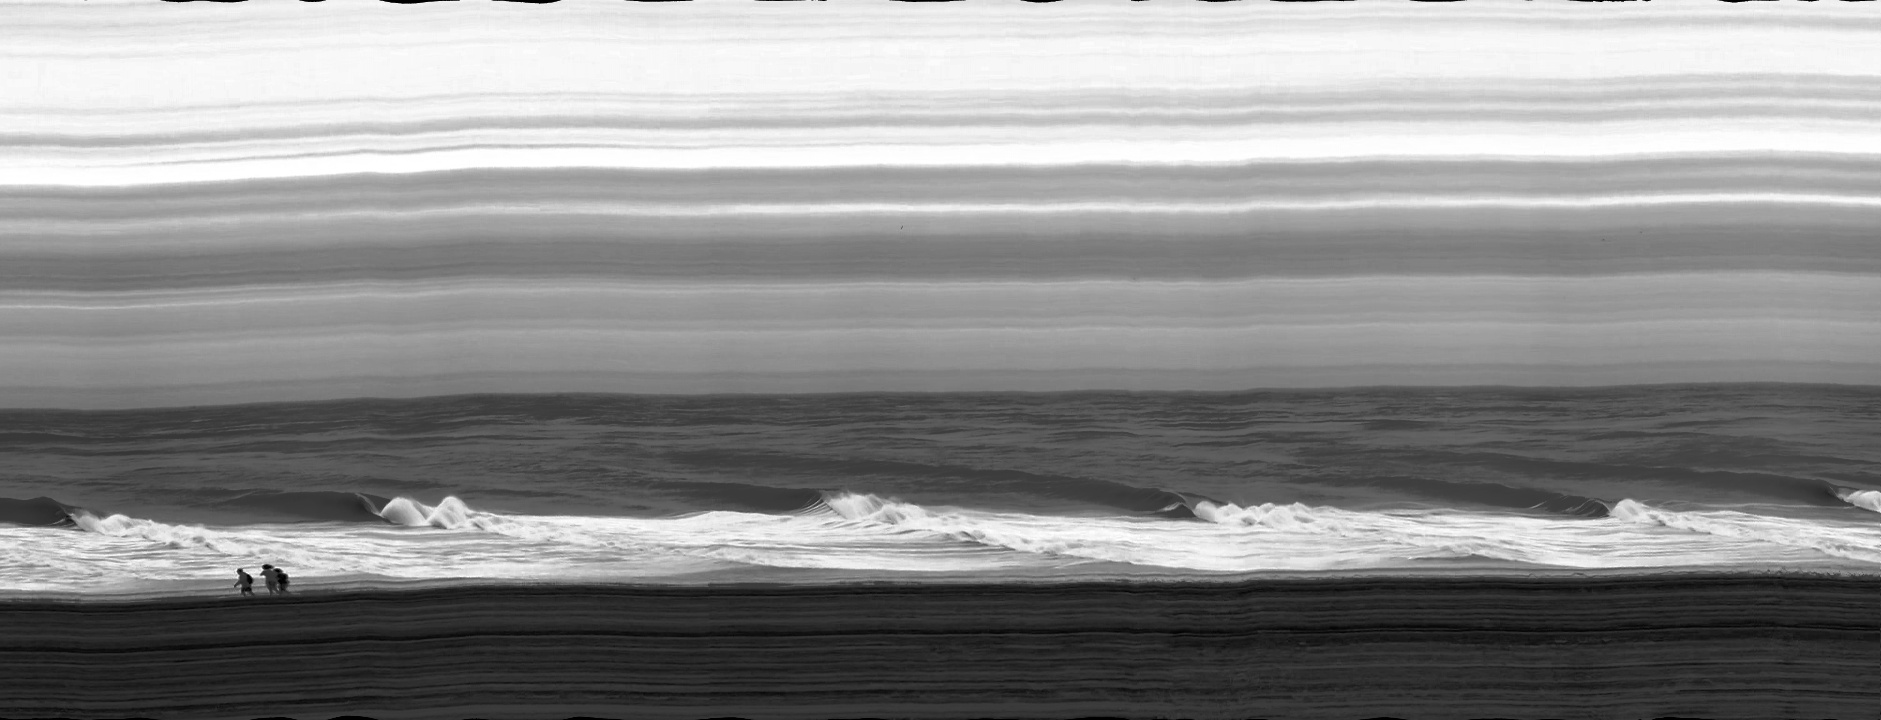
\includegraphics[width=.45\textwidth,keepaspectratio]{IMG_0798_2_stableTimestack.jpg}}
  \qquad
  \subfloat[\small{\textit{Timestack} gerado a partir de um v�deo gravado com ponto de montagem fixo.}]{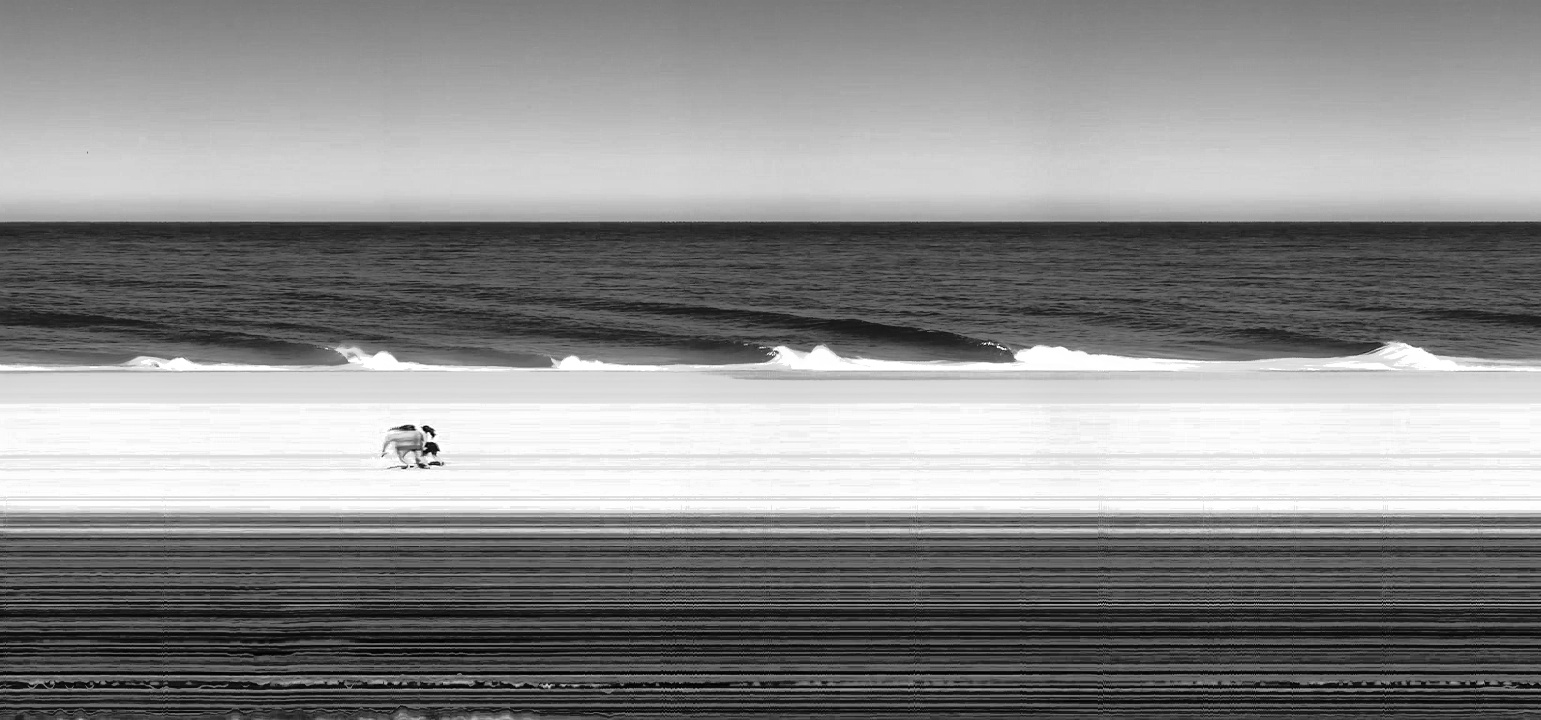
\includegraphics[width=.45\textwidth,keepaspectratio]{IMG_0896_cutted_originalTimestack.jpg}}
  \qquad
  \subfloat[\small{\textit{Timestack} gerado a partir de um v�deo gravado com ponto de montagem fixo e estabilizado por \textit{software}.}]{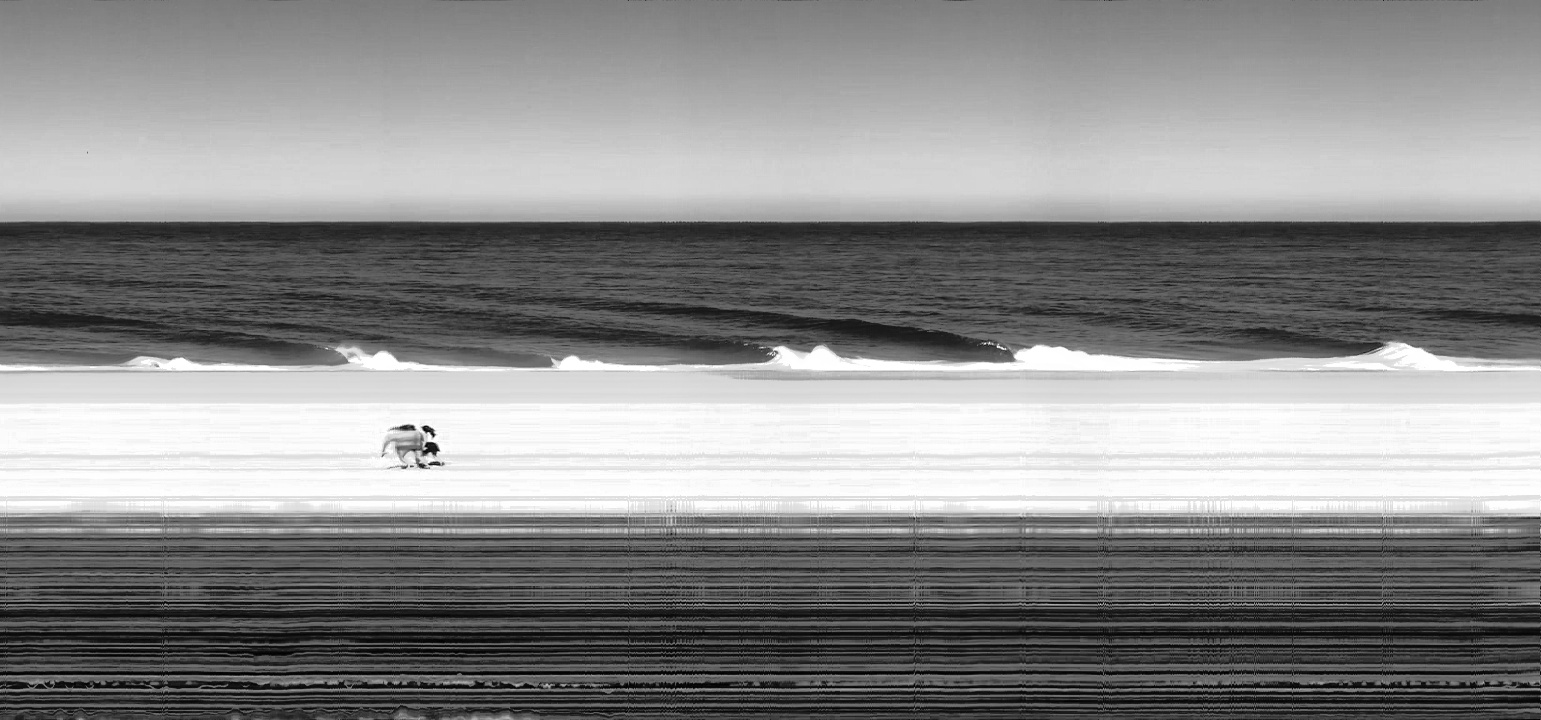
\includegraphics[width=.45\textwidth,keepaspectratio]{IMG_0896_cutted_stableTimestack.jpg}}
  \caption[\small{Compara��o entre \textit{timestack} gerado a partir de um v�deo gravado manualmente e o mesmo v�deo estabilizado. O c�u foi preservado para facilitar a compara��o da estabiliza��o.}]{\small{Compara��o entre \textit{timestack} gerado a partir de um v�deo gravado manualmente e o mesmo v�deo estabilizado. O c�u foi preservado para facilitar a compara��o da estabiliza��o.}}
  \label{FigStabilization}
\end{figure}

\section{Convers�o para N�vel de Cinza}

\paragraph{}Ap�s gerar o \timestack, o mesmo � convertido para n�vel de cinza. Os passos e etapas subsequentes do algoritmo ora proposto n�o necessitam trabalhar com cores, apenas a intensidade de cada \textit{pixel} � necess�ria para estimar a altura das ondas. O processamento das imagens se torna mais eficiente, pois a representa��o de uma imagem em n�vel de cinza possui um ter�o do tamanho de representa��o de imagem em cores. Com isso, o algoritmo utilizara menos mem�ria para executar e seu tempo de execu��o � reduzido.

\paragraph{}A convers�o para n�vel de cinza � realizada de acordo com a seguinte f�rmula \cite{Griffith14}:

\[
  I(t, v) = 0.35R(t, v) + 0.5G(t, v) + 0.15B(t, v)
\]

\noindent{}onde \(I(t,v)\) � a intensidade do pixel na posi��o \((t,v)\) na imagem convertida, e \(R(t,v)\), \(G(t,v)\) e \(B(t,v)\) s�o, respectivamente, os valores das componentes vermelhas, verdes e azuis do pixel \((t,v)\) da imagem original.

\section{Equaliza��o de Histograma}

\paragraph{}A equaliza��o de histograma tem como funcionalidade normalizar o n�vel intensidade da imagem. Desta forma, reduz-se tanto o efeito do clima (como a varia��o da ilumina��o em dias nublados e dias de c�u aberto) quanto o efeito do hor�rio do dia (como a varia��o da ilumina��o entre o come�o da manh� e o meio do dia). Al�m disso, nuvens e objetos externos podem alterar a ilumina��o durante a aquisi��o do v�deo em si. Portanto, deve-se equalizar o histograma de cada \textit{frame} do v�deo antes de gerar o \textit{timestack}.

%Descrever como � feita a equaliza��o, tal como voc� fez na se��o de n�veis de cinza.

\section{Detec��o da Linha de Horizonte}

\paragraph{}Uma etapa importante � a detec��o da linha de horizonte a fim de viabilizar a detec��o e remo��o do c�u na imagem. Esta opera��o � utilizada para facilitar o passo de \textit{thresholding} na etapa de processamento de imagem. Em alguns cen�rios, � dif�cil distinguir a regi�o de c�u da regi�o de arrebenta��o utilizando apenas o n�vel de intensidade dos \textit{pixels} de cada regi�o, pois a faixa de valores de intensidade de cada regi�o se sobrep�em. A figura \ref{FigTimestackFail}a exibe um \timestack com o c�u inclu�do ap�s aplicado um \textit{threshold} com valor de limite 150. Pode-se observar que parte do c�u n�o foi removido pelo \textit{threshold} (faixa branca na parte superior da imagem). J� a figura \ref{FigTimestackFail}b exibe um \timestack com o c�u inclu�do ap�s aplicado um \textit{threshold} com valor de limite 210. Com este valor o c�u foi removido completamente, mas a delimita��o da regi�o de espuma n�o foi bem definida, dificultando ou at� impossibilitando sua identifica��o (observe a faixa preta estreita presente na faixa branca da imagem). Por este motivo, a segmenta��o � baseada n�o s� no n�vel de intensidade dos \textit{pixels} mas como na sua localiza��o na imagem. A detec��o da linha de horizonte se mostra fundamental para obter localiza��o desta regi�o.

\begin{figure}[h]
  \centering
  \subfloat[\small{\textit{Timestack} sem remo��o do c�u (valor de \textit{threshold} 150)}]{
\includegraphics[width=\textwidth,keepaspectratio]{process_threshold_150.jpg}}
  \qquad
  \subfloat[\small{\textit{Timestack} sem remo��o do c�u (valor de \textit{threshold} 210)}]{
\includegraphics[width=\textwidth,keepaspectratio]{process_threshold_210.jpg}}
  \caption[\small{Compara��o do resultado do passo de \textit{thresholding} sem a remo��o do c�u.}]{\small{Compara��o do resultado do passo de \textit{thresholding} sem a remo��o do c�u.}}
  \label{FigTimestackFail}
\end{figure}

\paragraph{}A detec��o do c�u � realizada utilizando um detector de bordas de Canny para identificar a borda entre o c�u e o mar em um \textit{frame} do v�deo (Figura \ref{FigFrameCanny}). Ent�o, procura-se a primeira borda transversal detectada pelo m�todo de Canny, atrav�s do algoritmo descrito em \ref{AlgLineTracking}. A borda detectada corresponde a linha do horizonte. Todos os \textit{pixels} acima dessa linha s�o considerados como \textit{pixels} da regi�o do c�u, e ser�o removidos no passo seguinte.

\begin{figure}[h]
  \centering
  \subfloat[\small{\textit{Frame} do v�deo original.}]{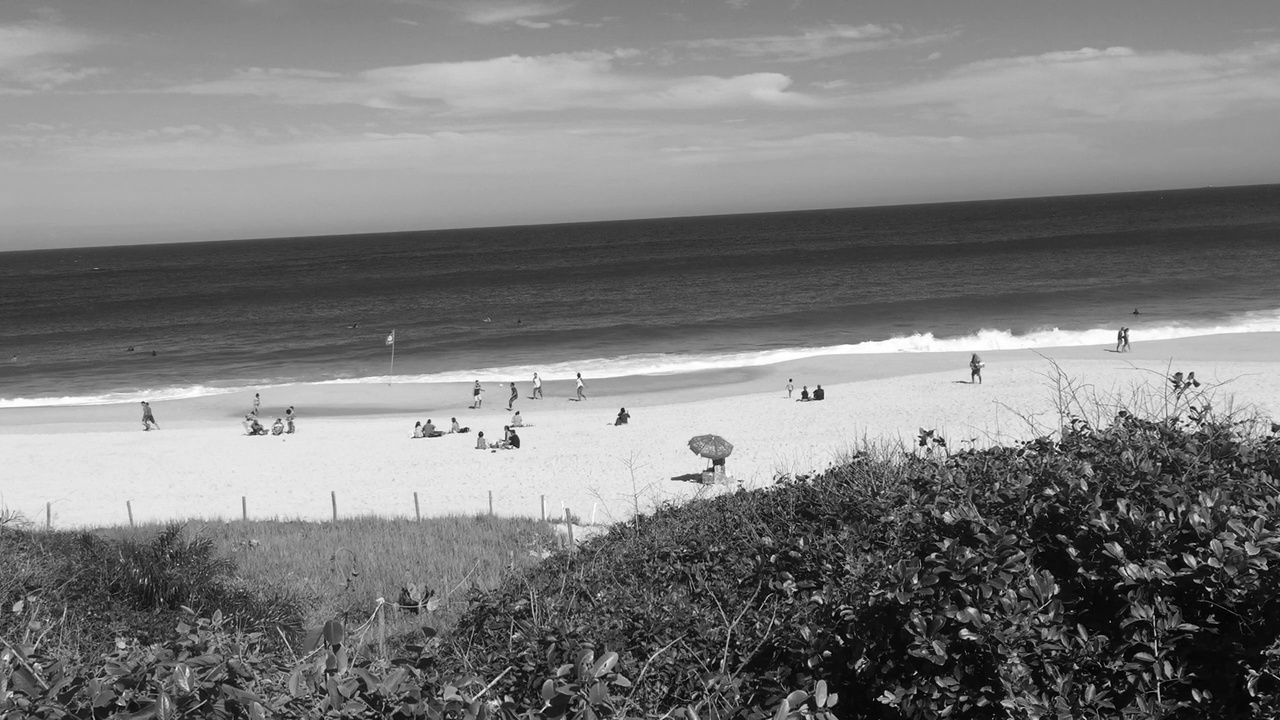
\includegraphics[width=0.45\textwidth,keepaspectratio]{simpletimestack_original.jpg}}
  \qquad
  \subfloat[\small{\textit{Frame} do v�deo com bordas detectadas pelo m�todo de Canny.}]{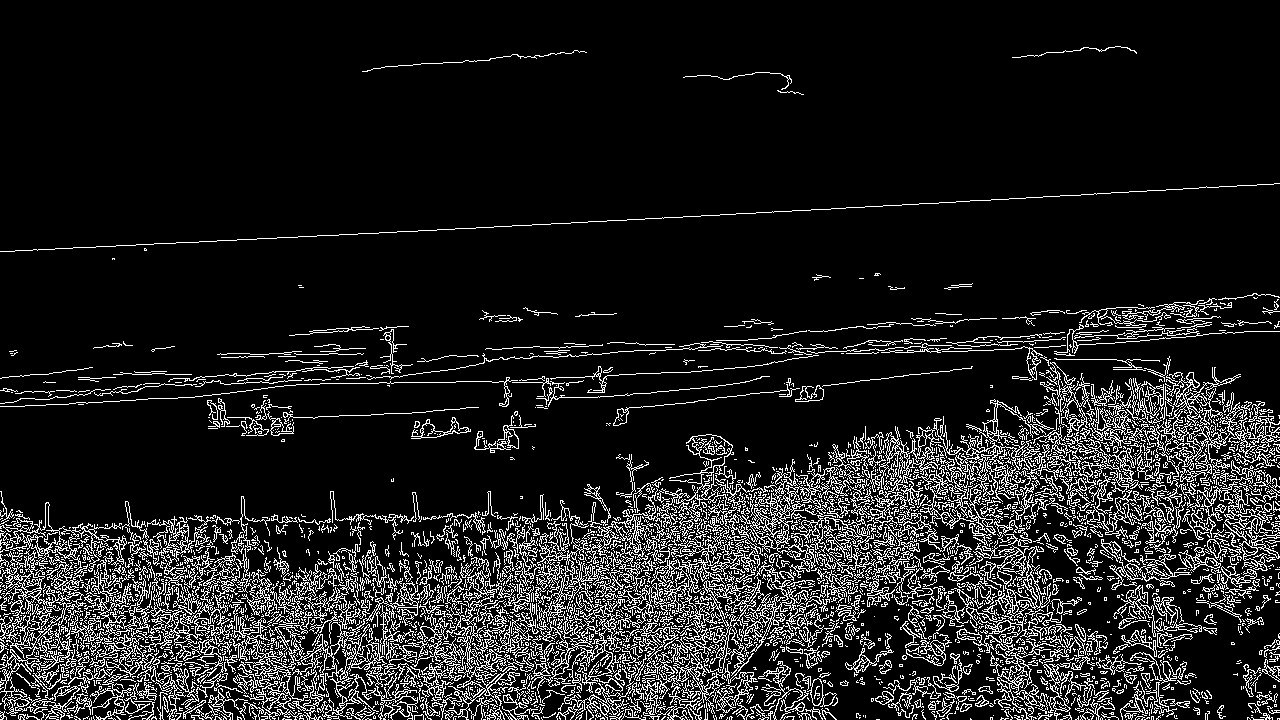
\includegraphics[width=0.45\textwidth,keepaspectratio]{simpletimestack_canny.jpg}}
  
  \caption[\small{Compara��o de um \textit{frame} original do v�deo com o mesmo \textit{frame} com as bordas detectadas pelo m�todo de Canny. A primeira borda transversal � a linha do horizonte.}]{\small{Compara��o de um \textit{frame} original do v�deo com o mesmo \textit{frame} com as bordas detectadas pelo m�todo de Canny. A primeira linha transversal na figura b � a linha do horizonte.}}
  \label{FigFrameCanny}
\end{figure}

\section{Remo��o do C�u}

\paragraph{}O �ltimo passo da etapa de pr�-processamento � a remo��o do c�u. Este passo utiliza duas entradas, a linha do horizonte detectada pelo passo anterior, e o \textit{frame} equalizado. A partir da linha do horizonte, considera-se todos os \textit{pixels} do \textit{frame} equalizado acima dessa linha como preto. A figura \ref{FigFrameSkyRemoved} exibe um \textit{frame} equalizado do v�deo original com o c�u removido.

\begin{figure}[h]
  \centering
  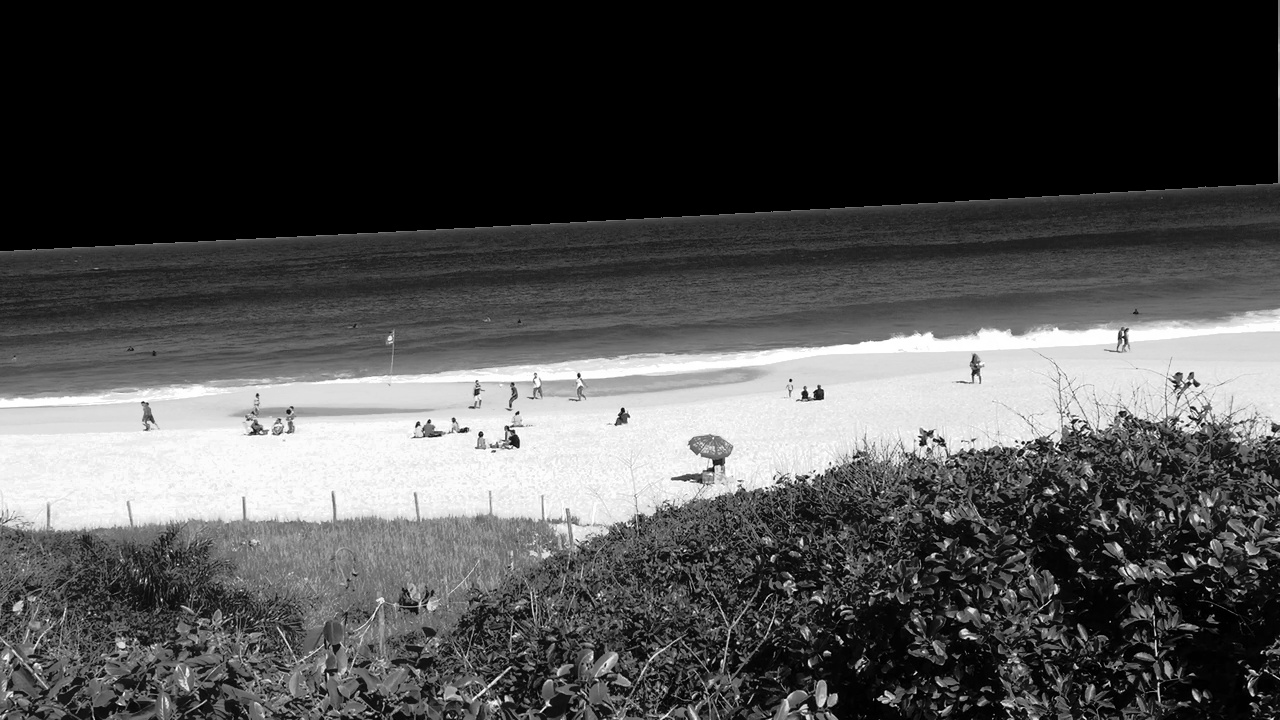
\includegraphics[width=0.8\textwidth,keepaspectratio]{simpletimestack_sky_removed.jpg}
  \caption[\small{\textit{Frame} equalizado com o c�u removido}]{\small{\textit{Frame} equalizado com o c�u removido}}
  \label{FigFrameSkyRemoved}
\end{figure}

\paragraph{}Como dito anteriormente, sem a remo��o do c�u, � dif�cil definir um valor �nico de \textit{threshold} que ser� utilizado na etapa de processamento principal. Uma tarefa essencial � ser capaz de separar o c�u, o mar e a faixa de espuma da arrebenta��o. Com o c�u removido, ao opera��o de \textit{threshold} produzir� resultados mais adequados para dar suporte �s etapas de medi��o.

\section{Processamento Principal}

\begin{figure}[h]
\begin{center}
  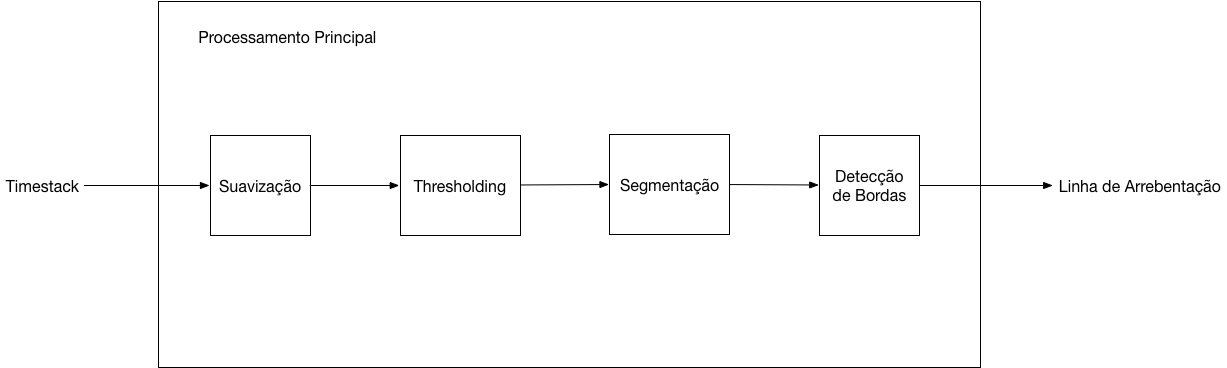
\includegraphics[width=\textwidth,height=\textheight,keepaspectratio]{diagrama_processamento.png}
  \caption[\small{Diagrama de Bloco da etapa de processamento principal.}]{\label{FigDiagramaProc} \small{Diagrama de Bloco da etapa de processamento principal.}}
\end{center}
\end{figure}

\paragraph{}A etapa de processamento principal tem como objetivo extrair a linha de arrebenta��o (figura \ref{FigLinhaArrebentacao}) de um \timestack gerado pelo pr�-processamento. A linha de arrebenta��o � definida como a linha que delimita a regi�o de espuma do restante do mar. Uma caracter�stica marcante dessas duas regi�es � que a regi�o de espuma apresenta a maioria dos \textit{pixels} com intensidade alta, enquanto o restante do mar apresenta a maioria dos \textit{pixels} com intensidade baixa. Esta caracter�stica ser� explorada para separar a regi�o de espuma do restante da imagem. Em seguida, a borda superior desta regi�o, que corresponde a linha de arrebenta��o, ser� analisada para identificar as ondas do mar presentes na imagem e medir a sua altura e periodicidade.

\begin{figure}[h]
  \centering
  \subfloat[\small{\textit{Timestack} gerado pelo pr�-processamento.}]{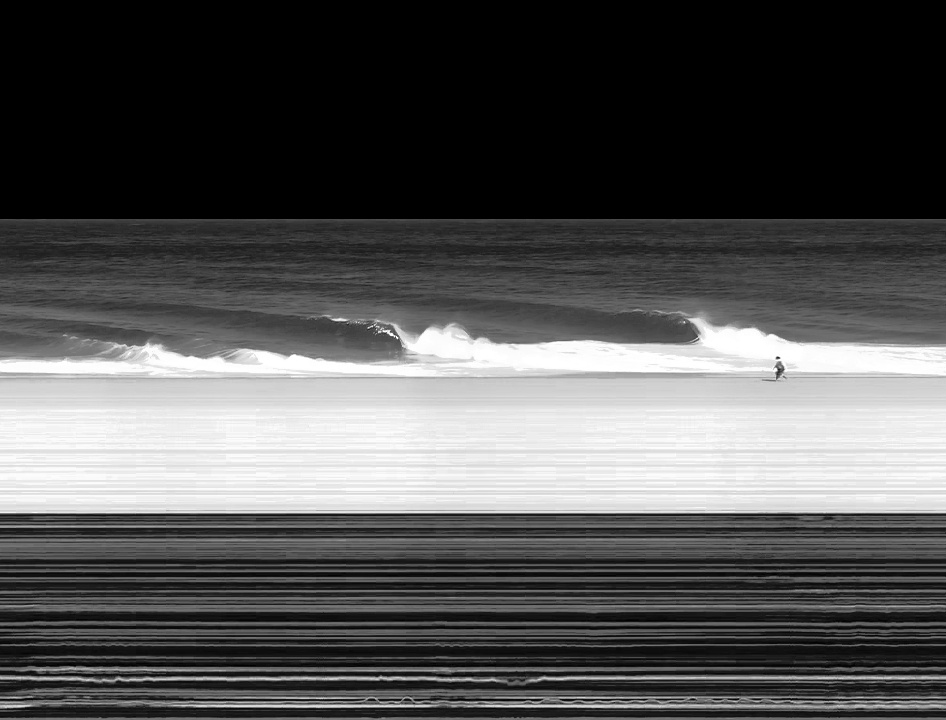
\includegraphics[width=0.45\textwidth,keepaspectratio]{breakzone_timestack.png}}
  \qquad
  \subfloat[\small{Linha de arrebenta��o detectada pelo processamento principal.}]{
\includegraphics[width=0.45\textwidth,keepaspectratio]{process_breakzone.png}}
  \caption[\small{Linha de arrebenta��o detectada pelo processamento principal.}]{ \small{Linha de arrebenta��o detectada pelo processamento principal.}}
  \label{FigLinhaArrebentacao}
\end{figure}

\paragraph{}As etapas de suaviza��o, \textit{thresholding}, segmenta��o e detec��o de bordas, que comp�e o Processamento Principal, ser�o descritas nas se��es a seguir.

\section{Suaviza��o}

\paragraph{}A primeira etapa de suaviza��o � realizada utilizando um filtro passa-baixas gaussiano, implementado no dom�nio do espa�o com m�scara de tamanho 15, valor escolhido empiricamente ap�s experimentar com imagens de diversos dias diferentes. Este efeito de suaviza��o � importante para reduzir o n�vel de ru�do na imagem, facilitando a identifica��o das bordas relevantes nos passos subsequentes. Outro efeito desejado � homogeneizar o n�vel de intensidade das regi�es da imagem, de forma que o passo de \textit{thresholding} consiga segmentar a regi�o de arrebenta��o do \timestack consistentemente. A figura \ref{FigGaussianBlurComparison} ilustra a diferen�a na segmenta��o da regi�o de espuma com e sem o passo de suaviza��o. A regi�o de espuma detectada est� marcada em vermelho. Nota-se que na figura \ref{FigGaussianBlurComparison}b a regi�o de espuma detectada � influenciada por pequenas faixas de alta intensidade espalhadas na regi�o do mar, enquanto a figura \ref{FigGaussianBlurComparison}a consegue filtrar essa influ�ncia e detectar uma regi�o de espuma mais uniforme.

\begin{figure}[h]
  \centering
  \subfloat[Regi�o de espuma detectada em um \textit{timestack} suavizado.]{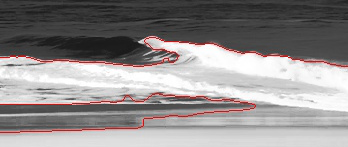
\includegraphics[width=0.8\textwidth,keepaspectratio]{waveband_blur.png}}
  \qquad
  \subfloat[Regi�o de espuma detectada em um \textit{timestack} n�o-suavizado.]{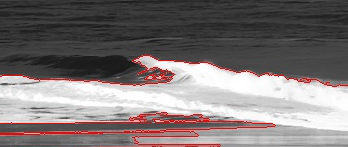
\includegraphics[width=0.8\textwidth,keepaspectratio]{waveband_no_blur.png}}
  \caption[\small{Compara��o da regi�o de espuma detectada com e sem suaviza��o.}]{\small{Compara��o da regi�o de espuma detectada com e sem suaviza��o.}}
  \label{FigGaussianBlurComparison} 
\end{figure}

%TODO: Adicionar imagem da primeira suaviza��o

\section{\textit{Thresholding}}

\paragraph{}\textit{Thresholding} � o primeiro passo para realizar a segmenta��o. Neste passo separa-se a regi�o de espuma do restante do mar, alterando todos os \textit{pixels} com intensidade abaixo de 150 para 0, e todos os \textit{pixels} acima deste valor para o valor de intensidade m�ximo. O valor limite foi escolhido empiricamente ap�s a an�lise de diversas imagens, contemplando dias variados. A figura \ref{FigThreshold} compara a regi�o de espuma detectada ap�s o passo de \textit{threshold} com valores diferentes. Pode-se notar na figura \ref{FigThreshold}a uma borda mais estreita sobre a regi�o de espuma observada, enquanto a figura \ref{FigThreshold}b exibe uma regi�o detectada n�o condizente com o resultado esperado. Inicialmente foi considerado um m�todo de decis�o do valor de \threshold din�mico, mas como discutido previamente, os passos de equaliza��o e remo��o do c�u realizados durante o pr�-processamento permitem utilizar um valor de \threshold est�tico, independente da condi��o de ilumina��o no momento da aquisi��o do v�deo. 

\paragraph{}Entretanto, dias muito nublados podem causar problemas para o \textit{thresholding}, como pode ser visto na figura \ref{FigThresholdFail}. Nesta figura os valores de intensidade da regi�o de espuma e da regi�o do mar no entorno das ondas se sobrep�e. Neste caso, o \threshold com valor est�tico n�o � capaz de separar as duas regi�es, impossibilitando a identifica��o das ondas do mar nos passos subsequentes.

\paragraph{}� importante notar que o \textit{thresholding} apenas isola as regi�es cujo n�vel de intensidade est� acima de um certo valor. Mais de uma regi�o pode ser isolada durante esse processo, por exemplo, partes da regi�o do mar pode estar mais clara que o esperado, e por isso ser�o preservadas pelo \threshold. O passo de segmenta��o � respons�vel por filtrar as regi�es isoladas pelo \textit{thresholding}.

\begin{figure}[h]
  \centering
  \subfloat[\small{Regi�o de espuma detectada usando \textit{threshold} no valor 150.}]{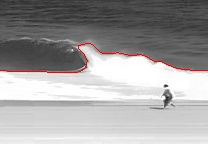
\includegraphics[width=.4\textwidth,keepaspectratio]{waveband_threshold_150.png}}
  \qquad
  \subfloat[\small{Regi�o de espuma detectada usando \textit{threshold} no valor 120.}]{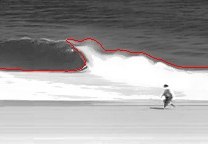
\includegraphics[width=.4\textwidth,keepaspectratio]{waveband_threshold_120.png}}
  \caption[\small{Trecho de um \textit{timestack} ap�s aplica��o de um \textit{threshold} com valores diferentes.}]{\small{Trecho de um \textit{timestack} ap�s aplica��o de um \textit{threshold} com valores diferentes.}
  \label{FigThreshold}
}
\end{figure}

\section{Segmenta��o e Detec��o de Bordas}

\paragraph{}O �ltimo passo do processamento principal � a segmenta��o. Este passo tem como objetivo identificar a regi�o de espuma dentre as regi�es isoladas pelo \textit{thresholding}, e identificar a sua borda externa para ser analisada pela pr�xima etapa. Primeiro, deve-se identificar todas as regi�es isoladas pelo \textit{thresholding}. Como a imagem est� binarizada, isto �, todos \textit{pixels} possuem a intensidade m�nima ou m�xima, as regi�es isoladas pelo \textit{thresholding} ser�o os conjuntos de \textit{pixels} cont�nuos com intensidade m�xima. Neste momento a biblioteca OpenCV agiliza a implementa��o pois � capaz de realizar a identifica��o das regi�es e a detec��o de bordas das mesmas de uma s� vez. Para isso utilizou-se a fun��o \textit{findContours}, que produz um vetor com todos contornos das regi�es isoladas pelo \textit{thresholding}.

\paragraph{}Em seguida, calcula-se a �rea de cada regi�o, a fim de encontrar a regi�o com a maior �rea. Novamente a biblioteca OpenCV se mostra uma escolha correta para este projeto, pois disponibiliza a fun��o \textit{contourArea} que c�lcula uma �rea de um contorno qualquer identificada pela fun��o \textit{findContours}. Para encontrar a maior regi�o basta percorrer o vetor de contornos obtidos anteriormente, calcular a �rea de cada elemento do vetor e preservar o �ndice o elemento de maior �rea (algoritmo \ref{AlgArea}).

\begin{algorithm}
  \caption{Algoritmo de Busca da Regi�o de Maior �rea}
  \label{AlgArea}
\begin{algorithmic}
\Procedure{EncontraMaiorArea}{vetor de contornos}
\State $indice \gets 0$
\State $maiorArea \gets 0$
\For{ contornos c no vetor de contornos } 
        \State $area \gets contourArea(c)$ \Comment Fun��o \textit{contourArea} do OpenCV
        \If {$ area > maiorArea $}
            \State $maiorArea \gets area$
            \State $indice \gets indice de c$
        \EndIf
\EndFor
\State retorna $indice$
\EndProcedure
\end{algorithmic}
\end{algorithm}

\paragraph{}Em condi��es normais a regi�o de maior �rea ser� a regi�o de espuma da imagem, ent�o pode-se descartar todas as outras regi�es. Por fim basta identificar as bordas da regi�o restante utilizando um m�todo de detec��o de bordas. Novamente, para facilitar a implementa��o foi utilizado o m�todo de Suzuki \cite{Suzuki85} para detec��o da borda, pois � o m�todo utilizado na fun��o \textit{findContours} da biblioteca OpenCV. Outro m�todo considerado para esta tarefa � o detector de bordas de Canny, j� utilizado no passo de detec��o da linha do horizonte, entretanto pela agilidade fornecida pelo OpenCV foi preterido em rela��o ao m�todo de Suzuki.

%Mostrar imagem da borda detectada com Suzuki e com Canny.

\section{An�lise e Identifica��o das Ondas Mar�timas}

\paragraph{}A �ltima etapa do algoritmo de estima��o da altura de ondas do mar � analisar a linha de arrebenta��o extra�da do \timestack e identificar as ondas do mar presentes nesta imagem. Feito isso, � poss�vel encontrar o ponto m�nimo e m�ximo locais da linha de arrebenta��o, que correspondem ao ponto m�nimo e m�ximo da onda em quest�o. Estas etapas s�o descritas nas se��es a seguir.

\begin{figure}[h]
\begin{center}
  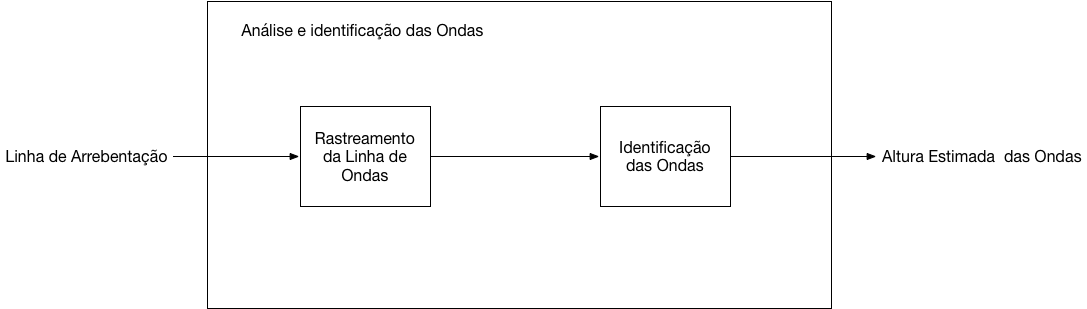
\includegraphics[width=\textwidth,height=\textheight,keepaspectratio]{diagrama_analise.png}
  \caption[\small{Diagrama de Bloco da etapa de an�lise. Fonte: Autor}]{\label{FigDiagramaAnalise} \small{Diagrama de Bloco da etapa de an�lise.}}
\end{center}
\end{figure}

\section{Rastreamento da Linha de Ondas}

\paragraph{}O primeiro passo desta etapa consiste em rastrear a linha de arrebenta��o encontrada, isto �, construir uma sequ�ncia \(s[n]\) que indica a sequ�ncia ordenada dos pontos \((x,y)\) que comp�e a linha de arrebenta��o. Esta sequ�ncia ordenada permite caminhar por cima da linha de arrebenta��o e assim determinar os pontos de m�ximo e m�nimo locais da linha.

\paragraph{}Para rastrear a linha de arrebenta��o foi utilizado um algoritmo que, dado um ponto de origem \(s[0] = (x_{i},y_{i})\), encontra o pr�ximo ponto da linha, o adiciona a sequ�ncia e busca o pr�ximo ponto, at� que n�o encontre mais nenhum ponto dispon�vel para adicionar na sequ�ncia \(s[n]\). O primeiro ponto � encontrado simplesmente percorrendo coluna a coluna da imagem, a partir da coluna mais � esquerda at� a coluna mais � direita at� que se encontre um ponto de intensidade maior que zero. Ent�o cria-se uma nova sequ�ncia com o ponto inicial igual ao ponto encontrado. O pseudo-c�digo \ref{AlgFirstPoint} ilustra o algoritmo que encontra e popula o primeiro ponto ($s[0]$) de uma sequ�ncia $s[n]$. 

\paragraph{}A busca do pr�ximo ponto ocorre na vizinhan�a imediata do �ltimo ponto da sequ�ncia, isto �, todos os oito pontos diretamente conectados ao ponto �ltimo ponto da sequ�ncia. Para cada ponto da sequ�ncia espera-se encontrar outros dois pontos em sua vizinhan�a, o ponto anterior e o ponto subsequente. Portanto, a an�lise da vizinhan�a deve desconsiderar o ponto anterior para n�o adicionar o mesmo ponto duas vezes na sequ�ncia. O ponto restante encontrado na vizinhan�a ser� o pr�ximo ponto, ent�o este ponto � adicionado ao final da sequ�ncia e o algoritmo se repete, at� que mais nenhum ponto seja encontrado. Entretanto, � poss�vel ocorrer descontinuidades na linha, isto �, um ponto na sequ�ncia possuir apenas um ou nenhum outro ponto em sua vizinhan�a imediata. Nesse caso, nenhum novo ponto ser� encontrado na vizinhan�a do �ltimo ponto da sequ�ncia, e o algoritmo ser� interrompido prematuramente. Para solucionar este problema se aumenta o raio da vizinhan�a e o algoritmo e repetido com o mesmo ponto central, buscando pontos mais distantes. Embora esta abordagem resolva os casos de descontinuidades pequenas, abre-se margem para que falsos positivos ocorram, isto �, pontos futuros sejam encontrados pulando o verdadeiro ponto subsequente. Para minimizar este problema, o raio de busca � limitado em um valor m�ximo igual a tr�s.

\paragraph{}Outro problema que atrapalha o funcionamento do algoritmo de rastreamento s�o casos onde um ponto possui mais de dois pontos em sua vizinhan�a. Este problema acontece quando existe um "la�o" na linha de arrebenta��o, e costuma ocorrer no momento que a onda quebra, e se torna mais comum a medida que o raio de busca aumenta. Nessa situa��o, considera-se o pr�ximo ponto simplesmente o primeiro ponto novo encontrado na vizinhan�a, e os demais pontos encontrados n�o s�o considerados. Por �ltimo, existem regi�es de espuma que o algoritmo n�o � capaz de rastrear a linha de arrebenta��o completamente, interrompendo a sequ�ncia prematuramente. Nesses casos, simplesmente inicia-se uma nova sequ�ncia a partir da coluna a direita do �ltimo ponto encontrado. Esse processo pode ser repetido in�meras vezes at� que se atinja a �ltima coluna da imagem. O pseudo-c�digo \ref{AlgLineTracking} ilustra o algoritmo de rastreamento que popula os pontos restantes de uma sequ�ncia $s[n]$.

\begin{algorithm}
  \caption{Algoritmo de Identifica��o do Primeiro Ponto da Linha}
  \label{AlgFirstPoint}
\begin{algorithmic}
\Procedure{EncontraPrimeiroPonto}{}
\For{cada coluna $c$ na borda da regi�o de espuma}
        \For{cada elemento $e$ na coluna $c$}
                \If{intensidade do elemento $e > 0$}
                        \State $s[0] = \text{posi��o do elemento } e$
                        \State{fim}
                \EndIf
        \EndFor
\EndFor
\EndProcedure
\end{algorithmic}
\end{algorithm}

\begin{algorithm}
  \caption{Algoritmo de Rastreamento de Linha}
  \label{AlgLineTracking}
\begin{algorithmic}
\Procedure{RastreiaLinha}{$raioDeBusca$}
\State $PontoAtual \gets s[N]$ \Comment{�ltimo ponto de s[n]}
\For{ pontos p ao redor de $PontoAtual$ em um raio de $raioDeBusca$ } 
        \If { $p \neq 0$ e $p$ n�o est� em $s[n]$ }
                \State $s[N+1] \gets p$
        \EndIf
\EndFor
\If{algum ponto foi adicionado a $s[n]$}
        \State{repetir o procedimento para o �ltimo ponto encontrado}
\Else
        \If{$raioDeBusca \leq 3$}
                \State{repetir o procedimento com $raioDeBusca+1$}
        \Else
                \State{fim}
        \EndIf
\EndIf
\EndProcedure
\end{algorithmic}
\end{algorithm}

\section{Identifica��o das Ondas}

\paragraph{}O �ltimo passo para estimar a altura das ondas em um \timestack � identificar as ondas na linha rastreada no passo anterior. Para isso, calcula-se a derivada da sequ�ncia discreta $s[n]$, da seguinte forma:

\[
  s'[n] = s[n] - s[n-1], \text{para n $>$ 0}
\] 

\noindent{}A sequ�ncia $s'[n]$ indica quais trechos da sequ�ncia original $s[n]$ s�o crescentes, decrescentes ou constantes. Ent�o, ao caminhar sobre a sequ�ncia derivada $s'[n]$, � trivial determinar quais s�o as faces crescentes das ondas. Em um cen�rio ideal, o ponto inicial de uma face crescente corresponde ao ponto m�nimo local de uma onda, e o �ltimo ponto crescente desta face corresponde ao ponto de m�ximo local, determinando assim a altura da onda. Entretanto, em uma imagem n�o ideal podem existir trechos que a derivada � $0$, ou at� mesmo negativa, antes da sequ�ncia tornar a crescer. A figura \ref{FigAutomato} descreve um aut�mato que reconhece uma onda considerando as condi��es descritas anteriormente.

\begin{figure}[h]
\begin{center}
  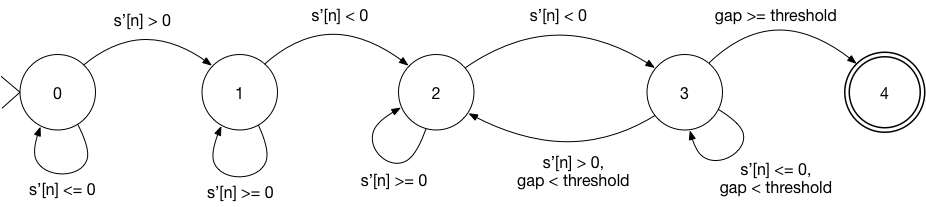
\includegraphics[width=\textwidth,height=\textheight,keepaspectratio]{automato_identificacao_onda.png}
  \caption[\small{Aut�mato Finito Determin�stico que identifica uma onda em uma linha de arrebenta��o.}]{\label{FigAutomato} \small{Aut�mato Finito Determin�stico que identifica uma onda em uma linha de arrebenta��o.}}
\end{center}
\end{figure}

\noindent{}O estado 0 do aut�mato procura pela primeira derivada $s'[n]$ positiva, marcando o ponto equivalente de $s[n]$ como o m�nimo da onda e avan�ando para o estado 1. O estado 1 procura pela primeira derivada negativa de $s'[n]$, marcando o ponto equivalente de $s[n]$ como candidato ao ponto m�ximo da onda e andando para o estado 2. Ent�o, os estados 2 e 3 buscam por "buracos" ou \textit{gaps} no trecho de derivada positiva, onde a derivada se torna negativa por um curto per�odo e depois $s[n]$ torna a crescer. O estado 2 procura por novos pontos de m�ximo, trechos onde a derivada � positiva, e o estado 3 procura por trechos de derivada negativa. Quando o estado 3 encontrar uma derivada positiva, o aut�mato retorna para o estado 2. Enquanto o estado 3 encontrar derivadas n�o-positivas um contador de tamanho do \textit{gap} � incrementado. Quando o tamanho do \textit{gap} � superior a um certo limite, o aut�mato avan�a para o estado 4, identificando assim que um candidato a uma onda foi encontrado, delimitado pelos pontos de m�nimo e m�ximo encontrados anteriormente. Este candidato apenas ser� considerado uma onda se sua altura estiver dentro de uma faixa de controle, isto �, s�o descartadas ondas muito pequenas ou muito grandes. A figura \ref{FigWave} mostra os pares de pontos m�ximo e m�nimo identificados pelo aut�mato em uma linha de arrebenta��o aplicados no \timestack original. As linhas verdes unem os pares de pontos encontrados, e as linhas vermelhas evidencia a altura em \textit{pixels} da onda identificada. 

\begin{figure}[h]
\begin{center}
  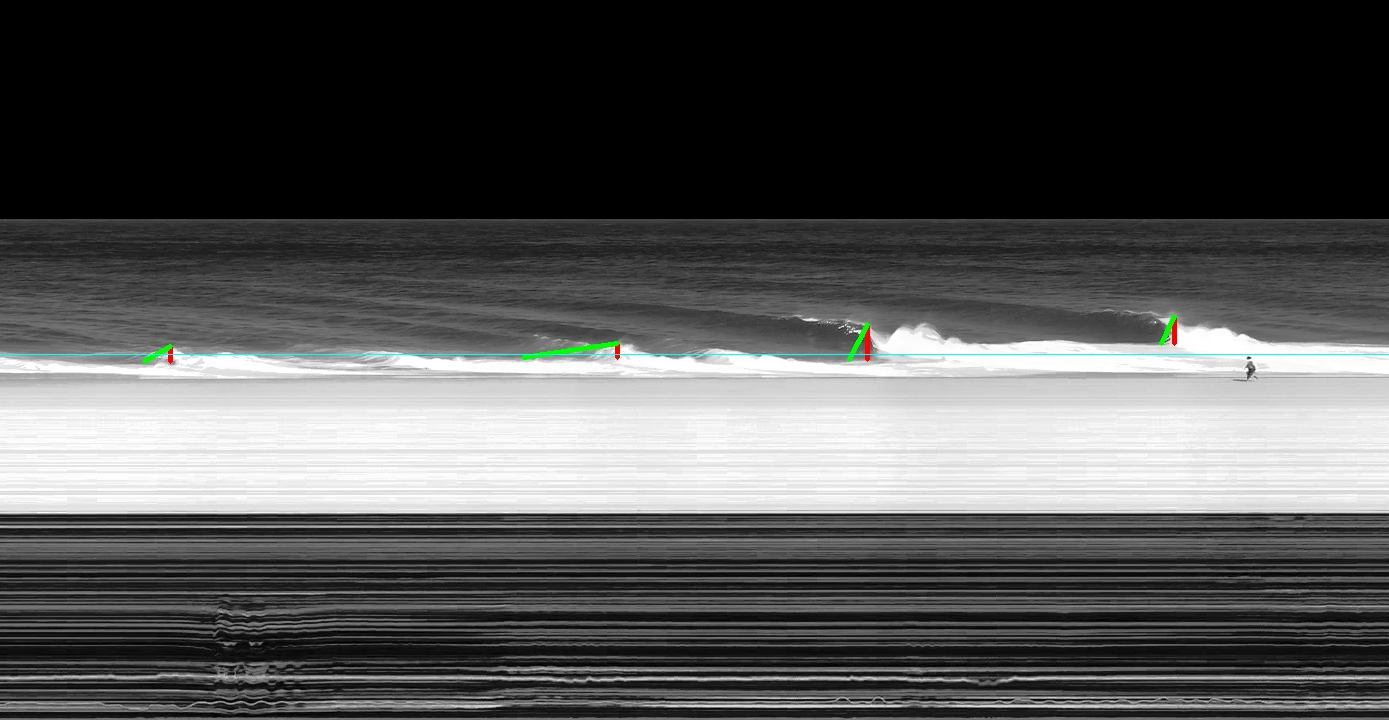
\includegraphics[width=\textwidth,height=\textheight,keepaspectratio]{process_waves_result.png}
  \caption[\small{Ondas identificadas pelo aut�mato.}]{\label{FigWave} \small{Ondas identificadas pelo aut�mato.}}
\end{center}
\end{figure}


% ---------------------------------------------------------------
% Chapter 4 - Implementa��o do Algoritmo
% ---------------------------------------------------------------
\chapter{Implementa��o do Algoritmo}
\label{cap4}
\lstset { %
    language=C++,
	breaklines=true,
	showstringspaces=false,
	backgroundcolor=\color{black!5}, % set backgroundcolor
	keywordstyle=\color{blue},
	breakatwhitespace=false,
	basicstyle=\footnotesize,
	rangeprefix=/*---,
	rangesuffix=---*/,
  	includerangemarker=false,
  	tabsize=2,
}

% Introdu��o implementa��o
\paragraph{}Este cap�tulo apresentar� a implementa��o do algoritmo discutido no Cap�tulo 3. Como introduzido anteriormente, a biblioteca de processamento gr�fico OpenCV foi utilizada para agilizar a implementa��o do projeto, as pr�ximas se��es apresentar�o como a biblioteca foi utilizada para implementar cada etapa do projeto.

%Introdu��o OpenCV
\paragraph{}A biblioteca OpenCV \cite{OpenCVOrg} (\textit{Open Source Computer Vision Library}) � uma biblioteca de aprendizado de m�quina e vis�o computacional, distribu�da sob a licen�a BSD, livre para o desenvolvimento de aplica��es acad�micas e comerciais. Ela foi projetada para ser computacionalmente eficiente e tem foco em aplica��es em tempo real. Esta biblioteca implementa diversos algoritmos de vis�o computacional e aprendizado de m�quina (mais de 2500 algoritmos implementados \cite{OpenCVAbout}), incluindo a grande maioria dos algoritmos descritos nos Cap�tulos 2 e 3. A biblioteca oferece interface de desenvolvimento nas linguagens de programa��o C++, Python e Java. Para este projeto de gradua��o a linguagem de programa��o escolhida foi a linguagem C++, por dois motivos: das tr�s linguagens � a com melhor performance e � a linguagem que o autor possui maior familiaridade.

%Mat
\paragraph{}O OpenCV apresenta uma estrutura chamada Mat \cite{OpenCVMat} para representar uma matriz qualquer. Esta estrutura ser� amplamente utilizada no projeto pois � a estrutura que representa uma imagem. As suas propriedades mais importantes s�o:

\begin{enumerate}
	\item N�mero de linhas e n�mero de colunas - determina o comprimento e largura da imagem.

	\item Tipo de elemento da matriz - determina se cada elemento da matriz ser� um char sem sinal ou um \textit{float} / \textit{double}.

	\item N�mero de canais - determina se cada elemento da matriz ser� representado com um �nico valor (n�vel de cinza) ou com tr�s valores (sistema de cores RGB).
\end{enumerate}

\noindent{}Neste projeto a maiorias dos Mats utilizados ser�o do tipo char sem sinal e com apenas um canal. Em determinados momentos as matrizes s�o convertidas para tr�s canais apenas para facilitar a depura��o de algum processo intermedi�rio do projeto, como na figura \ref{FigThreshold} onde � desej�vel exibir uma imagem com cores para visualizar etapas diferentes do projeto sobre a mesma imagem (nessa figura a regi�o de espuma em vermelho sobre o \textit{timestack} original para verificar se a identifica��o foi correta).

\section{Pr�-Processamento}

%Leitura do v�deo do filesystem
\paragraph{}O pr�-processamento inicia pela leitura de um v�deo no \textit{filesystem}. A leitura do v�deo � realizada pela fun��o \textit{imread}. Esta fun��o aceita um par�metro: uma \textit{string} contendo o caminho no \textit{filesystem} para encontrar o v�deo desejado. Esta fun��o pode retornar um objeto do tipo Mat (quando o arquivo lido � uma imagem) ou um objeto do tipo VideoCapture (quando o objeto lido � um v�deo). O objeto VideoCapture � uma estrutura de dados que representa um v�deo. Para este projeto as propriedades mais importantes dessa estrutura s�o o n�mero de \textit{frames} por segundo e a dura��o do v�deo. O n�mero de \textit{frames} por segundo ser� utilizado posteriormente para converter a posi��o no eixo horizontal das ondas encontradas no \textit{timestack} em valores temporais, ou seja, quantos segundos ap�s o in�cio do v�deo as ondas quebraram.

\paragraph{}A partir de um objeto VideoCapture � poss�vel obter um objeto Mat que representa cada \textit{frame} do v�deo, atrav�s do operador de deslocamento a esquerda. Pode-se iterar por todos os \textit{frames} do v�deo em um la�o \textit{while} da seguinte forma:

\begin{lstlisting}
// Lendo v�deo do filesystem
cv::VideoCapture videoCapture = cv::imread("caminho no filesystem"); 
while (true) { // La�o para iterar sobre as frames do v�deo
	Mat frame;
	videoCapture >> frame;

	// Se frame.data == NULL o la�o chegou no final do v�deo
	if (frame.data == NULL) 
		break;

	// frame pronto para realizar alguma opera��o
}
\end{lstlisting}

%Convers�o para n�vel de cinza
\paragraph{}Uma vez obtido cada \textit{frame} do v�deo, pode-se implementar o \textit{pipeline} exibido na figura \ref{FigDiagramaPreProc}b. Primeiro, converte-se o \textit{frame} originalmente colorido para n�vel de cinza. Isto � realizado pela fun��o \textit{cv::cvtColor}. Esta fun��o aceita tr�s par�metros: um objeto Mat de entrada, um objeto Mat de sa�da (onde ser� guardado o resultado da fun��o) e um valor enumerado representando a representando a opera��o de convers�o que ser� realizada - \textit{COLOR\_BGR2GRAY} para converter uma imagem no sistema RGB em n�vel de cinza e \textit{COLOR\_GRAY2BGR} para converter uma imagem em n�vel de cinza para sistema RGB. O c�digo abaixo exemplifica o uso desta fun��o ao converter um \textit{frame} colorido para n�vel de cinza:

\begin{lstlisting}
Mat greyFrame;
cv::cvtColor(frame,greyFrame,COLOR_BGR2GRAY);
\end{lstlisting}

%Equaliza��o
\paragraph{}Ap�s alterar o sistema de cores do \textit{frame}, o pr�ximo passo � equalizar o seu histograma. O uso da biblioteca OpenCV apresenta uma vantagem neste passo pois a fun��o \textit{equalizeHist} calcula o histograma de um objeto Mat de entrada e j� o equaliza com apenas uma �nica chamada de fun��o. Esta fun��o aceita dois par�metros: o objeto Mat de entrada que ser� equalizado em um outro objeto Mat onde ser� guardado o resultado da opera��o. � importante observar que est� fun��o opera apenas sobre objetos Mat com um canal, isto �, em n�vel de cinza. O c�digo abaixo exemplifica o uso desta fun��o, equalizando um \textit{frame} em n�vel de cinza:

\begin{lstlisting}
Mat equalizedFrame;
cv::equalizeHist(greyFrame,equalizedFrame);
\end{lstlisting}

%Detec��o da Linha do Horizonte
\paragraph{}A detec��o da linha do horizonte � realizada sobre o \textit{frame} em n�vel de cinza n�o equalizado. Como discutido no cap�tulo anterior, � necess�rio realizar primeiro um passo de detec��o de bordas com o m�todo de Canny e ent�o detectar a primeira linha transversal na imagem atrav�s do algoritmo \ref{AlgLineTracking}. Primeiro, para detectar as bordas com o algoritmo de Canny utiliza-se a fun��o \textit{Canny} da biblioteca OpenCV. Esta fun��o recebe quatro par�metros: um objeto Mat de entrada, um objeto Mat de sa�da, um \textit{double} que representa o valor de \textit{threshold} inferior e um \textit{double} que representa o valor de \textit{threshold} superior. O c�digo abaixo exemplifica o uso desta fun��o:

\begin{lstlisting}
Mat edgeFrame;
double lowThreshold = 50.0;
double highThreshold = 150.0;
cv::Canny(greyFrame,edgeFrame,lowThreshold,hightThreshold);
\end{lstlisting}

\paragraph{}Em seguida busca-se pelo primeiro ponto n�o nulo na primeira coluna da imagem. Em condi��es normais espera-se que este ponto esteja logo na primeira coluna da imagem, uma vez que a linha de horizonte deve sempre abranger toda o comprimento horizontal da imagem. O c�digo abaixo demonstra como esta busca � implementada:

\begin{lstlisting}
for (int y = 0; y < edgeFrame.rows; y++) {
	uchar value = edgeFrame.at<uchar>(y,0);
	if (value > 0) { // valor n�o nulo
		// primeiro ponto encontrado
		break;
	}
}
\end{lstlisting}

\noindent{}Uma vez encontrado o primeiro ponto, utiliza-se o algoritmo \ref{AlgLineTracking} para rastrear o restante da linha at� o final do comprimento horizontal da imagem. Para representar as linhas detectadas por este algoritmo foi criado uma classe Trajectory. Esta classe cumpre tr�s fun��es b�sicas para este projeto:

\begin{enumerate}
	\item Implementa os algoritmos de rastreamento de uma linha \ref{AlgFirstPoint} e \ref{AlgLineTracking}.

	\item Mant�m um vetor ordenado com os pontos encontrados pelos algoritmos de rastreamento de linha.

	\item Calcula a derivada do seu vetor de pontos ordenados.
\end{enumerate}

\noindent{}A fim de melhorar a organiza��o do projeto, criou uma classe denominada Derivable para implementar as fun��es 2 e 3 descritas anteriormente. A classe Trajectory herda essas caracter�sticas da classe Derivable. Para representar cada ponto das classes Derivable e Trajectory criou-se uma classe Point. O diagrama \ref{DiagTrajectory} apresenta interface de cada classe e demonstra a rela��o entre as tr�s.

\begin{figure}[h]
	\centering
	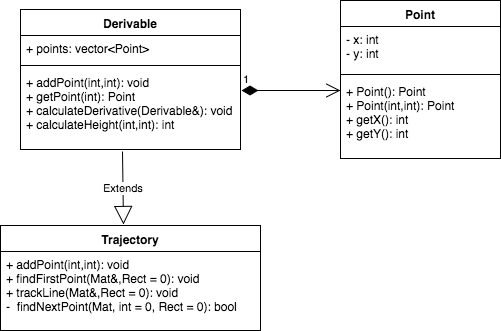
\includegraphics[width=0.8\textwidth,keepaspectratio]{class_diagram_trajectory.png}
	\caption[\small{Diagrama das classes Derivable, Trajectory e Point.}]{\small{Diagrama das classes Derivable, Trajectory e Point.}}
	\label{DiagTrajectory}
\end{figure}

\paragraph{}O c�lculo da derivada de uma lista de pontos � implementada no m�todo Derivable::calculateDerivative conforme o c�digo abaixo:

\lstinputlisting[linerange=calculateDerivativeBegin-calculateDerivativeEnd]{../src/include/derivable.hpp}

\paragraph{}O algoritmo \ref{AlgFirstPoint} � implementado no m�todo Trajectory::findFirstPoint(cv::Mat\&,cv::Rect) conforme o c�digo abaixo:

\begin{lstlisting}
void Trajectory::findFirstPoint(cv::Mat& mat, cv::Rect roi) {
	int width = mat.cols;
	int height = mat.rows;

	for (int i = (1+roi.x); i < (roi.x + roi.width - 1); i++) {
		Mat col = mat.col(i);

		bool found = false;
		for (int j = (roi.y); j < (roi.y+roi.height - 1); j++) {
			if (col.at<uchar>(j) > 0) {
				found = true;
				addPoint(i,j);
				break;
			}
		}

		if (found)
			break;

	}	
}
\end{lstlisting}

\noindent{}O par�metro mat define qual a imagem onde o m�todo deve procurar pelo primeiro ponto. O m�todo Trajectory::addPoint verifica se este ponto j� foi adicionado ao vetor de pontos do objeto Trajectory, e em caso negativo o adiciona ao final do vetor. O par�metro roi define uma regi�o retangular que � a regi�o de interesse sobre a qual o m�todo operar�. O primeiro ponto deve ser procurado dentro da regi�o definida pelo par�metro roi. Caso o par�metro roi seja omitido, a regi�o interesse considerada ser� a imagem inteira.

\paragraph{}O algoritmo \ref{AlgLineTracking} � implementado nos m�todos Trajectory::trackLine(cv::Mat\&,cv::Rect) e Trajectory::findNextPoint(cv::Mat\&,int,cv::Rect), conforme o c�digo abaixo:

\begin{lstlisting}
void Trajectory::trackLine(Mat& m, Rect roi) {
	while(true)
		if (! findNextPoint(m,1,roi))
			break;
}

bool Trajectory::findNextPoint(Mat& m, int radius, Rect roi) {
	Point currentPoint = points.back();

	if (currentPoint.getX() >= (roi.x + roi.width - 1))
		return false;

	int MAX_RADIUS = 3;

	int beginY = currentPoint.getY() - radius > (roi.y) ? currentPoint.getY() - radius : roi.y;
	int endY = currentPoint.getY() + radius < (roi.y + roi.height - 1) ? currentPoint.getY() + radius : roi.y + roi.height - 1;

	int beginX = currentPoint.getX() - radius > (roi.x) ? currentPoint.getX() - radius : roi.x;
	int endX = currentPoint.getX() + radius < (roi.x + roi.width - 1) ? currentPoint.getX() + radius : roi.x + roi.width - 1;

	for (int i = beginX; i <= endX; i++)
		for (int j = beginY; j <= endY; j++)
			if (m.at<uchar>(j,i) > 0 && addPoint(i,j))
				return true;

	if (radius < MAX_RADIUS)
		return findNextPoint(m,radius+1,roi);

	return false;
}
\end{lstlisting}

\noindent{}Novamente o par�metro mat define qual a imagem onde o m�todo deve procurar pelo pr�ximo ponto, e o par�metro roi � a regi�o de interesse na imagem que delimita a regi�o onde o m�todo deve procurar pelo ponto. O par�metro radius indica qual � o raio de busca do algoritmo, isto �, qu�o dist�nte do �ltimo ponto encontrado o m�todo deve procurar por um ponto novo. Como no m�todo Trajectory::findFirstPoint(cv::Mat\&,cv::Rect) o par�metro roi pode ser omitido, assumindo ent�o que a regi�o de interesse � a imagem inteira. O par�metro radius pode ser omitido tamb�m, neste caso assume-se o valor de raio igual a um, que � menor raio poss�vel.

%Remo��o do C�u
\paragraph{}O �ltimo passo realizado sobre cada \textit{frame} � a remo��o do c�u. Este passo � realizado baseado na linha do horizonte rastreada no passo anterior e no \textit{frame} equalizado obtido na etapa de equaliza��o de histograma. Basta ent�o percorrer todos os \textit{pixels} do \textit{frame} equalizado, e alterar o valor de intensidade dos \textit{pixels} acima da linha de horizonte detectada para zero. O c�digo abaixo ilustra como esse passo � realizado:

\begin{lstlisting}
Trajectory trajectory;
Rect roi(0,0,1,edgeFrame.rows);
trajectory.findFirstPoint(edgeFrame,roi);
trajectory.trackLine();
for (int i = 0; i < trajectory.points.size(); i++) {
	Point p = trajectory.getPoint(i);
	for (int j = 0; j < p.getY(); j++) {
		equalizedFrame.at<uchar>(j,i) = 0;
	}
}
\end{lstlisting}

\noindent{}Onde a vari�vel edgeFrame � um objeto Mat resultante do passo de detec��o de linha do horizonte, e a vari�vel equalizedFrame � o objeto Mat resultante do passo de equaliza��o de histograma.

\paragraph{}Como este passo � realizado para todos os \textit{frames} do v�deo, � poss�vel otimiz�-lo, aproveitando-se do fato que a estabilidade do v�deo � garantida no momento da sua captura. O fato do v�deo ser est�vel implica que a linha do horizonte sempre estar� na mesma posi��o \textit{frame} a \textit{frame}, ent�o n�o � necess�rio detectar uma nova linha do horizonte para cada \textit{frame} do v�deo, basta identifica-la uma �nica vez e utiliz�-la para remover o c�u de todos os \textit{frames}. Durante o processamento do primeiro \textit{frame} monta-se um objeto Mat do mesmo tamanho do \textit{frame} que servir� como uma m�scara. Ent�o, uma vez detectada a linha do horizonte, altera-se a m�scara de forma que todos os \textit{pixels} abaixo da linha do horizonte possuam valor de intensidade m�ximo e todos os \textit{pixels} acima da linha do horizonte tenham intensidade m�nima. O c�digo abaixo mostra como montar a m�scara :

\begin{lstlisting}
Trajectory trajectory;
cv::Rect roi(0,0,1,edgeFrame.rows);
trajectory.findFirstPoint(edgeFrame,roi);
trajectory.trackLine();

cv::Mat skyRemoverMask = cv::Mat::ones(equalizedFrame.size(),equalizedFrame.type());

for (int i = 0; i < trajectory.points.size(); i++) {
	Point p = trajectory.getPoint(i);
	for (int j = 0; j < p.getY(); j++) {
		skyRemoverMask.at<uchar>(j,i) = 0;
	}
}
\end{lstlisting}

\noindent{}Para remover o c�u aplica-se a m�scara a cada \textit{frame} equalizado atrav�s do m�todo Mat::copyTo(Mat,Mat). Este m�todo copia um objeto Mat para outro, sendo que uma m�scara pode ser especificada com o segundo par�metro para definir quais \textit{pixels} do objeto original ser�o copiados. O c�digo abaixo ilustra como esta fun��o � utilizada em conjunto com a m�scara criada anteriormente:

\begin{lstlisting}
cv::Mat skyRemovedFrame;
equalizedFrame.copyTo(skyRemovedFrame,skyRemoverMask);
\end{lstlisting}

%Timestack
\paragraph{}O �ltimo passo do pr�-processamento � a gera��o do \textit{timestack} a partir dos \textit{frames} processados. Como discutido no Cap�tulo 3, um \textit{timestack} � formado pelo acumulo de uma mesma coluna de cada \textit{frame} de um v�deo. Ent�o, para formar um \textit{timestack} gen�rico basta iterar por todos os \textit{frames} de um v�deo, selecionar uma coluna com o mesmo �ndice de cada \textit{frame} e o acumula-lo em um �nico objeto Mat. O c�digo abaixo exibe como gerar um \textit{timestack} gen�rico que acumula a coluna central de cada \textit{frame}:

\begin{lstlisting}
cv::VideoCapture videoCapture = cv::imread("caminho no filesystem"); 

// O m�todo VideoCapture::get obt�m um propriedade do v�deo
// especificada pelo segundo par�metro
int frameHeight = videoCapture.get(cv::CV_CAP_PROP_FRAME_HEIGHT); 

// O terceiro par�metro (cv::CV_8UC1) especifica o tipo e n�mero de canais
// do objeto Mat que ser� criado.
cv::Mat timestack(0,frameHeight,cv::CV_8UC1,0);

while (true) {
	cv::Mat frame;
	videoCapture >> frame;

	if (frame.data == NULL) 
		break;

	// O m�todo Mat::col retorna a coluna do �ndice especificado 
	// como par�metro.
	cv::Mat middleColumn = frame.col(frame.cols/2);

	// O m�todo Mat::push_back adiciona par�metro Mat ao final do
	// objeto Mat que est� sendo aplicado.
	timestack.push_back(middleColumn);
}
\end{lstlisting}

\paragraph{}Os passos descritos at� aqui comp�em juntos o pr�-processamento completo, como ilustrado a seguir:

\begin{lstlisting}[tabsize=2]
// Lendo o v�deo do filesystem
cv::VideoCapture videoCapture = cv::imread("caminho no filesystem"); 

int frameWidth = videoCapture.get(cv::CV_CAP_PROP_FRAME_WIDTH); 
int frameHeight = videoCapture.get(cv::CV_CAP_PROP_FRAME_HEIGHT); 

// Criando objeto Mat que ir� guardar o timestack
cv::Mat timestack(0,frameHeight,cv::CV_8UC1,0);

// Criando objeto Mat que ir� guardar a m�scara de remo��o do c�u
cv::Mat skyRemoverMask = cv::Mat::ones(cv::Size(frameWidth,frameHeight),cv::CV_8UC1);
bool isMaskReady = false;

// Iterando sobre os frames do v�deo
while (true) {
	cv::Mat frame;
	videoCapture >> frame;

	// Verificando se o frame � v�lido
	if (frame.data == NULL) 
		break;

	// Convers�o para n�vel de cinza
	Mat greyFrame;
	cv::cvtColor(frame,greyFrame,COLOR_BGR2GRAY);

	// Se a m�scara n�o estiver pronta (primeira execu��o),
	// � necess�rio detectar a linha do horizonte
	if (! isMaskReady) {
		// Detec��o da linha do horizonte
		Mat edgeFrame;
		double lowThreshold = 50.0;
		double highThreshold = 150.0;
		cv::Canny(greyFrame,edgeFrame,lowThreshold,hightThreshold);

		// Constru��o da m�scara para remo��o da linha do horizonte
		Trajectory trajectory;
		cv::Rect roi(0,0,1,edgeFrame.rows);
		trajectory.findFirstPoint(edgeFrame,roi);
		trajectory.trackLine();

		cv::Mat skyRemoverMask = cv::Mat::ones(equalizedFrame.size(),equalizedFrame.type());

		for (int i = 0; i < trajectory.points.size(); i++) {
			Point p = trajectory.getPoint(i);
			for (int j = 0; j < p.getY(); j++) {
				skyRemoverMask.at<uchar>(j,i) = 0;
			}
		}

		// Alterando o valor da vari�vel para otimiza��o
		isMaskReady = true;
	}

	// Equalizando o frame
	Mat equalizedFrame;
	cv::equalizeHist(greyFrame,equalizedFrame);

	// Remo��o do C�u
	cv::Mat skyRemovedFrame;
	equalizedFrame.copyTo(skyRemovedFrame,skyRemoverMask);

	// Gerando o timestack
	cv::Mat middleColumn = equalizedFrame.col(equalizedFrame.cols/2);
	timestack.push_back(middleColumn);
}
\end{lstlisting}

\section{Processamento Principal}

\paragraph{}O processamento principal, como discutido no cap�tulo anterior, opera sobre um \textit{timestack} gerado pelo pr�-processamento e tem como sa�da a linha de arrebenta��o da regi�o de espuma do \textit{timestack}. Tamb�m foi discutido que o pr�-processamento e o processamento principal podem ocorrer em dispositivos diferentes, o pr�-processamento no aparato de \textit{hardware} que realiza a captura do v�deo e o processamento principal em um servidor na nuvem. Dito isso, o primeiro passo do processamento principal � a leitura de um \textit{timestack} no \textit{filesystem}. Assim como no pr�-processamento, a leitura � feita pela fun��o \textit{imread}. O c�digo abaixo exemplifica como isto � feito:

\begin{lstlisting}
cv::Mat timestackMat = cv::imread("caminho para o timestack");
\end{lstlisting}

%Suaviza��o
\paragraph{}O passo de suaviza��o � o primeiro passo realizado ap�s a leitura do \textit{timestack} do \textit{filesystem}. Para isso � utilizada a fun��o \textit{GaussianBlur} que aceita quatro par�metros: um objeto Mat de entrada, um objeto Mat de sa�da, um objeto Size indicando o tamanho da m�scara do filtro gaussiano, um valor double indicando o desvio padr�o da m�scara do filtro gaussiano. O c�digo abaixo ilustra como est� fun��o � utilizada:

\begin{lstlisting}
cv::Size kernelSize(15,15);
double standardDeviation = 0;
cv::Mat blurredMat;
cv::GaussianBlur(timestackMat,blurredMat,kernelSize,standardDeviation);
\end{lstlisting}

%Thresholding
\paragraph{}A seguir � realizada o passo de \textit{thresholding}. Este passo � realizado utilizando a fun��o \textit{threshold}, que recebe cinco par�metros: um objeto Mat de entrada, um objeto Mat de sa�da, um valor double indicando o valor limite do \textit{threshold}, um valor double indicando qual � o valor m�ximo utilizado em \textit{threshold} de binariza��o, e um valor inteiro indicando qual o tipo de \textit{threshold} que ser� aplicado. O tipo de \textit{threshold} pode ser combinado com a sinaliza��o cv::CV\_THRESH\_OTSU para utilizar o m�todo de Otsu para calcular o valor do limite. Neste caso, o valor double indicando o limiar de \textit{threshold} deve ser 0. Neste projeto ser� utilizado o tipo cv::CV\_THRESH\_BINARY com o m�todo de Otsu. O c�digo abaixo exibe como esta fun��o � utilizada:

\begin{lstlisting}
double thresholdLimit = 0;
double maxValue = 255;
cv::Mat thresholdedMat;
cv::threshold(blurredMat,thresholdedMat,thresholdLimit,maxValue,cv::CV_THRESH_BINARY | cv::CV_THRESH_OTSU);
\end{lstlisting}

% \noindent{}O tipo de \textit{thresholding} cv::THRESH_BINARY indica que qualquer \texit{pixel} do objeto Mat de entrada com valor de intensidade acima do valor limite ser� alterado para o valor m�ximo, e qualquer \texit{pixel} do objeto Mat de entrada com valor de intensidade abaixo do valor limite ser� alterado para zero.

% Segmenta��o e Detec��o de Bordas
\paragraph{}O �ltimo passo do processamento principal � a segmenta��o e a detec��o de bordas. Um pouco da implementa��o deste passo j� foi discutido no Cap�tulo 3. � utilizada a fun��o \textit{findContours} para identificar as regi�es isoladas pelo \textit{thresholding} e detectar as suas bordas, e em seguida a fun��o \textit{contourArea} � utilizada para selecionar dentre as regi�es identificadas qual � a regi�o de maior �rea. Por �ltimo, a fun��o \textit{drawContours} � utilizada para formar um objeto Mat com apenas a borda da regi�o de espuma. A fun��o \textit{findContours} recebe cinco par�metros: um objeto Mat de entrada, um de vetor de vetores de objetos Point indicando os contornos encontrados, um vetor de vetores de inteiros indicando a rela��o de hierarquia entre os contornos, um inteiro indicando o modo de opera��o e um inteiro indicando o m�todo de aproxima��o de contornos. Os modos de opera��o poss�veis s�o: 

%cv::CV_RETR_EXTERNAL, cv::CV_RETR_LIST, cv::CV_RETR_CCOMP e cv::CV_RETR_TREE. Os m�todos de aproxima��o poss�veis s�o: cv::CV_CHAIN_APPROX_NONE, cv::CV_CHAIN_APPROX_SIMPLE, cv::CV_CHAIN_APPROX_TC89_L1 e cv::CV_CHAIN_APPROX_TC89_KCOS. O c�digo abaixo exibe como a fun��o \textit{findContours} � utilizada:

\begin{lstlisting}
vector< vector<cv::Point> > contours;
vector<cv::Vec4i> hierarchy;
findContours( thresholdedMat, contours, hierarchy, cv::CV_RETR_CCOMP, cv::CV_CHAIN_APPROX_SIMPLE );
\end{lstlisting}


%cv::CV_RETR_CCOMP
\noindent{}O modo de opera��o  organiza os contornos encontrados em dois n�veis: contornos externos e contornos internos. Desta forma, � poss�vel eliminar "buracos" dentro da regi�o de espuma que podem surgir na opera��o de \textit{thresholding}. Em seguida, a �rea de cada contorno encontrado � calculada e ent�o determina-se a regi�o de maior utilizando a fun��o \textit{contourArea}. Esta fun��o recebe dois par�metros: um vetor de objetos Point indicando o contorno que ser� calculado a �rea, e um valor boleano indicando se a �rea � orientada ou n�o. O c�digo abaixo ilustra como esta fun��o � utilizada:

\begin{lstlisting}
vector<cv::Point> contour;
// ...
double area = contourArea(contour,false);
\end{lstlisting}

\noindent{}Dado um vetor de contornos (vetor de vetores de objetos Point), pode-se determinar o contorno de maior �rea com o c�digo abaixo:

\begin{lstlisting}
double largest_area = 0;
double largest_contour_index = 0;
for (int i = 0; i< contours.size(); i++) {
   double area = contourArea(contours[i],false);
   if (area > largest_area) {
       largest_area = area;
       largest_contour_index = i;
    }
}
\end{lstlisting}

\noindent{}Por �ltimo � criado um objeto Mat contendo apenas o maior contorno encontrado atrav�s da fun��o \textit{drawContours}. Esta fun��o recebe quatro par�metros: um objeto Mat de sa�da, um vetor de contornos contendo todos os contornos detectados, um inteiro indicando o �ndice do contorno que deve ser desenhado no objeto Mat e um objeto Color indicando a cor que deve ser desenhado. O c�digo abaixo ilustra como est� fun��o � utilizada:

\begin{lstlisting}
cv::Scalar color( 255, 255, 255 );
cv::Mat contourMat(thresholdedMat.rows,thresholdedMat.cols,cv::CV_8UC1,cv::Scalar::all(0));
cv::drawContours( contourMat, contours, largest_contour_index, color );
\end{lstlisting}

\paragraph{}O processamento principal pode ser implementado por completo unindo os passos apresentados nesta se��o, coforme o c�digo abaixo:

\begin{lstlisting}
// Lendo imagem do filesystem
cv::Mat timestackMat = cv::imread("caminho para o timestack");

// Suaviza��o
cv::Size kernelSize(15,15);
double standardDeviation = 0;
cv::Mat blurredMat;
cv::GaussianBlur(timestackMat,blurredMat,kernelSize,standardDeviation);

// Threshold
double thresholdLimit = 150;
double maxValue = 255;
cv::Mat thresholdedMat;
cv::threshold(blurredMat,thresholdedMat,thresholdLimit,maxValue,cv::THRESH_BINARY);

// Identifica��o dos Contornos
vector< vector<cv::Point> > contours;
vector<cv::Vec4i> hierarchy;
findContours( thresholdedMat, contours, hierarchy, cv::CV_RETR_CCOMP, cv::CV_CHAIN_APPROX_SIMPLE );

// Determina��o da maior regi�o
double largest_area = 0;
double largest_contour_index = 0;
for (int i = 0; i< contours.size(); i++) {
   double area = contourArea(contours[i],false);
   if (area > largest_area) {
       largest_area = area;
       largest_contour_index = i;
    }
}

// Gera��o o objeto Mat com apenas o contorno desejado
cv::Scalar color( 255, 255, 255 );
cv::Mat contourMat(thresholdedMat.rows,thresholdedMat.cols,cv::CV_8UC1,cv::Scalar::all(0));
cv::drawContours( contourMat, contours, largest_contour_index, color );
\end{lstlisting}

\section{An�lise e Identifica��o de Ondas Mar�timas}

\paragraph{}A �ltima etapa do algoritmo � a an�lise e identifica��o das ondas mar�timas. Esta etapa opera sobre a linha de arrebenta��o resultante do processamento principal e tem como resultado a altura estimada de cada onda identificada. 

%Rastreamento da Linha de Ondas
\paragraph{}O primeiro passo a ser realizado � o rastreamento da linha de arrebenta��o. Neste passo � utilizada a mesma classe de rastreamento de linhas utilizada para detec��o da linha do horizonte no pr�-processamento, a classe Trajectory. Ao contr�rio da linha do horizonte, a linha de arrebenta��o n�o ser� uma linha reta, ent�o � poss�vel que o algoritmo de rastreamento implementado na classe Trajectory encontre um trecho da linha que ele n�o � capaz de rastrear. Nesses casos, interrompe-se o rastreamento at� este ponto, as ondas neste trecho s�o identificadas e ent�o o algoritmo de rastreamento reinicia na coluna seguinte ao ponto em que parou, buscando novamente um ponto inicial e rastreando o restante da linha a partir deste ponto. O rastreamento s� termina quando o algoritmo chega at� o final da linha, isto �, at� que o �ltimo ponto da linha rastreada esteja na extremidade direita da imagem analisada. O c�digo abaixo ilustra como o rastreamento da linha de arrebenta��o � implementado:

\begin{lstlisting}
// Imagem com a linha de arrebenta��o encontrada na etapa de processamento principal
cv::Mat contourMat = imread("caminho no filesystem");

// Vari�vel que guarda qual a �ltima coluna analisada
int lastCol = 0;

while(true) {

	if (lastCol >= contourMat.cols-1) {
		break;
	}

	Trajectory trajectory(contourMat,Rect(lastCol,0,contourMat.cols - col, contourMat.rows));

	// Objeto Trajectory pronto para an�lise	

	// Atualizando vari�vel com a coluna seguinte a �ltima coluna do objeto Trajectory
	lastCol = trajectory.points.back().getX() + 1;
}
\end{lstlisting}

\begin{figure}[h]
	\centering
	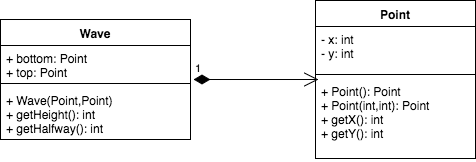
\includegraphics[width=0.8\textwidth,keepaspectratio]{class_diagram_wave.png}
	\caption[\small{Diagrama da classe Wave.}]{\small{Diagrama da classe Wave.}}
	\label{DiagramWave}
\end{figure}

%Identifica��o das Ondas
\paragraph{}O �ltimo passo a ser realizado � a identifica��o das ondas mar�timas. Este passo � realizado implementando o automato descrito no cap�tulo anterior (Figura \ref{FigAutomato}). O automato de identifica��o das ondas foi implementado em uma fun��o analyseTrajectory, conforme o c�digo abaixo:

\lstinputlisting[tabsize=2,linerange=analyseTrajectoryBegin-analyseTrajectoryEnd]{../src/lib/waveDetector.cpp}

\noindent{}A fun��o detectWave utilizada na fun��o analyseTrajectory verifica se um par de pontos identificados como pontos m�nimos e m�ximos locais s�o eleg�veis para formar uma onda. Para serem eleg�veis, cada par de pontos devem atender 2 requisitos:

\begin{enumerate}
	\item A diferen�a de altura do par de pontos deve estar dentro de uma faixa limite, para impedir que anomalias sejam identificadas como ondas. Os valores limites m�ximo e m�nimo s�o, respectivamente: 10 e 200.

	\item O ponto m�nimo detectado deve estar � direita do �ltimo ponto m�ximo detectado. Isto se deve pois o eixo horizontal da linha de arrebenta��o representa o eixo temporal, e sempre deve evoluir da esquerda para a direita. Portanto novas ondas devem sempre estar mais � direita de ondas j� identificadas. Esta verifica��o � �til para evitar que a turbul�ncia causada pela arrebenta��o da onda gere falsos-positivos, ou seja uma onda seja erroneamente detectada em decorr�ncia da arrebenta��o de outra onda.
\end{enumerate}

\noindent{}O c�digo abaixo exibe como a fun��o detectWave � implementada:

\lstinputlisting[linerange=detectWaveBegin-detectWaveEnd]{../src/lib/waveDetector.cpp}

\paragraph{}A fun��o analyseTrajectory implementa o m�todo de corre��o do ponto m�nimo das ondas discutido no cap�tulo 3. Ela utiliza uma fun��o auxiliar fixBottomPoint que � implementada conforme o c�digo a seguir:

\lstinputlisting[linerange=fixBottomPointBegin-fixBottomPointEnd]{../src/lib/waveDetector.cpp}

\paragraph{}O resultado deste automato � um vetor de objetos Wave (figura \ref{DiagramWave}), um objeto criado pelo autor que representa um par de pontos indicando o ponto mais baixo e o ponto mais alto de uma onda. A classe Wave implementa dois m�todos: o m�todo getHeight, que calcula a diferen�a de altura da onda em \textit{pixels}, e o m�todo getHalfway, que calcula o ponto central horizontal da onda.

\paragraph{}Por fim, a altura das ondas em \textit{pixels} � convertida para medidas do mundo real, em metros. Esta convers�o � realizada baseado no m�todo apresentado na se��o \ref{sec:camera}. O c�digo abaixo ilustra como as equa��es descritas na se��o \ref{sec:camera} foram implementadas:

\lstinputlisting[linerange=calculateAngleBegin-calculateAngleEnd]{../src/include/camera.hpp}
\lstinputlisting[linerange=calculateRealHeightBegin-calculateRealHeightEnd]{../src/include/camera.hpp}

\noindent{}A altura das ondas identificadas na linha de arrebenta��o pode ser calculada conforme o c�digo abaixo:

\begin{lstlisting}
double cameraAngle, focalAngle, cameraHeight;
int imageHeight = contourMat.rows;

for (int i = 0; i < detectedWaves.size(); i++) {
	double realWorldHeight = calculateRealHeight(detectedWaves[i].top.getY(),dectectedWaves[i].bottom.getY(),cameraHeight,cameraAngle,focalAngle,imageHeight);
}
\end{lstlisting}

\noindent{}As vari�veis cameraAngle, focalAngle e cameraHeight s�o par�metros conhecidos da filmagem, medidos no momento da captura do v�deo.

% ---------------------------------------------------------------
% Chapter 5 - Dados Experimentais
% ---------------------------------------------------------------
\chapter{Dados Experimentais}
\label{cap5}
\paragraph{}Este cap�tulo tem como objetivo apresentar os resultados obtidos ao aplicar o m�todo de estima��o de altura de ondas discutido nos cap�tulos 2 e 3. 

\paragraph{}Os v�deos analisados foram capturados na praia de Itacoatiara, em Niter�i. A c�mera foi posicionada no Quiosque 5, na orla da praia, a uma altura de aproximadamente oito metros do n�vel do mar. Este quiosque foi escolhido para posicionar a c�mera pois uma vis�o clara do mar, sem a obstru��o da vegeta��o local da praia. A c�mera est� posicionada com uma angula��o vertical de 83$^{\circ}$. Os v�deos foram capturados tanto utilizando \textit{smartphones} do tipo iPhone quanto o aparato de \textit{hardware} apresentado nos cap�tulos 3 e 4. De acordo com o modelo de praia apresentado por Browne \textit{et al}, o �nico par�metro intr�nseco das c�meras utilizado para calcular as alturas reais � o campo de vis�o. O campo de vis�o (\textit{field of view}) da c�mera do \textit{smartphone} foi calculado atrav�s da seguinte equa��o \cite{Bourke}: 

\[
	fov = 2 * atan\Bigg(\frac{h}{2f}\Bigg)
\]

\noindent{}onde $h$ � a altura da imagem no sensor da c�mera e $f$ � a dist�ncia focal da c�mera. Estes par�metros foram obtidos no momento da captura atrav�s do pr�prio \textit{smartphone}. Os valores considerados foram:

\begin{center}
    \begin{tabular}{| c | c |}
	    \hline
	    Par�metros & Valores \\ \hline
	    Dist�ncia Focal & 4.15 mm\\ \hline
	    Altura do sensor & 3.60 mm\\ \hline
	    Campo de vis�o vertical & 46.92$^{\circ}$ \\ 
	    \hline
    \end{tabular}
\end{center}

\noindent{}O campo de vis�o da c�mera utilizada no aparato de \textit{hardware} possui campo de vis�o vertical fixo, com o valor de $41.41^{\circ}$ \cite{RaspberryCamera}.

\begin{figure}[h]
    \centering
    \subfloat[\small{Quiosque 5 e a praia de Itacoatiara ao fundo.}]{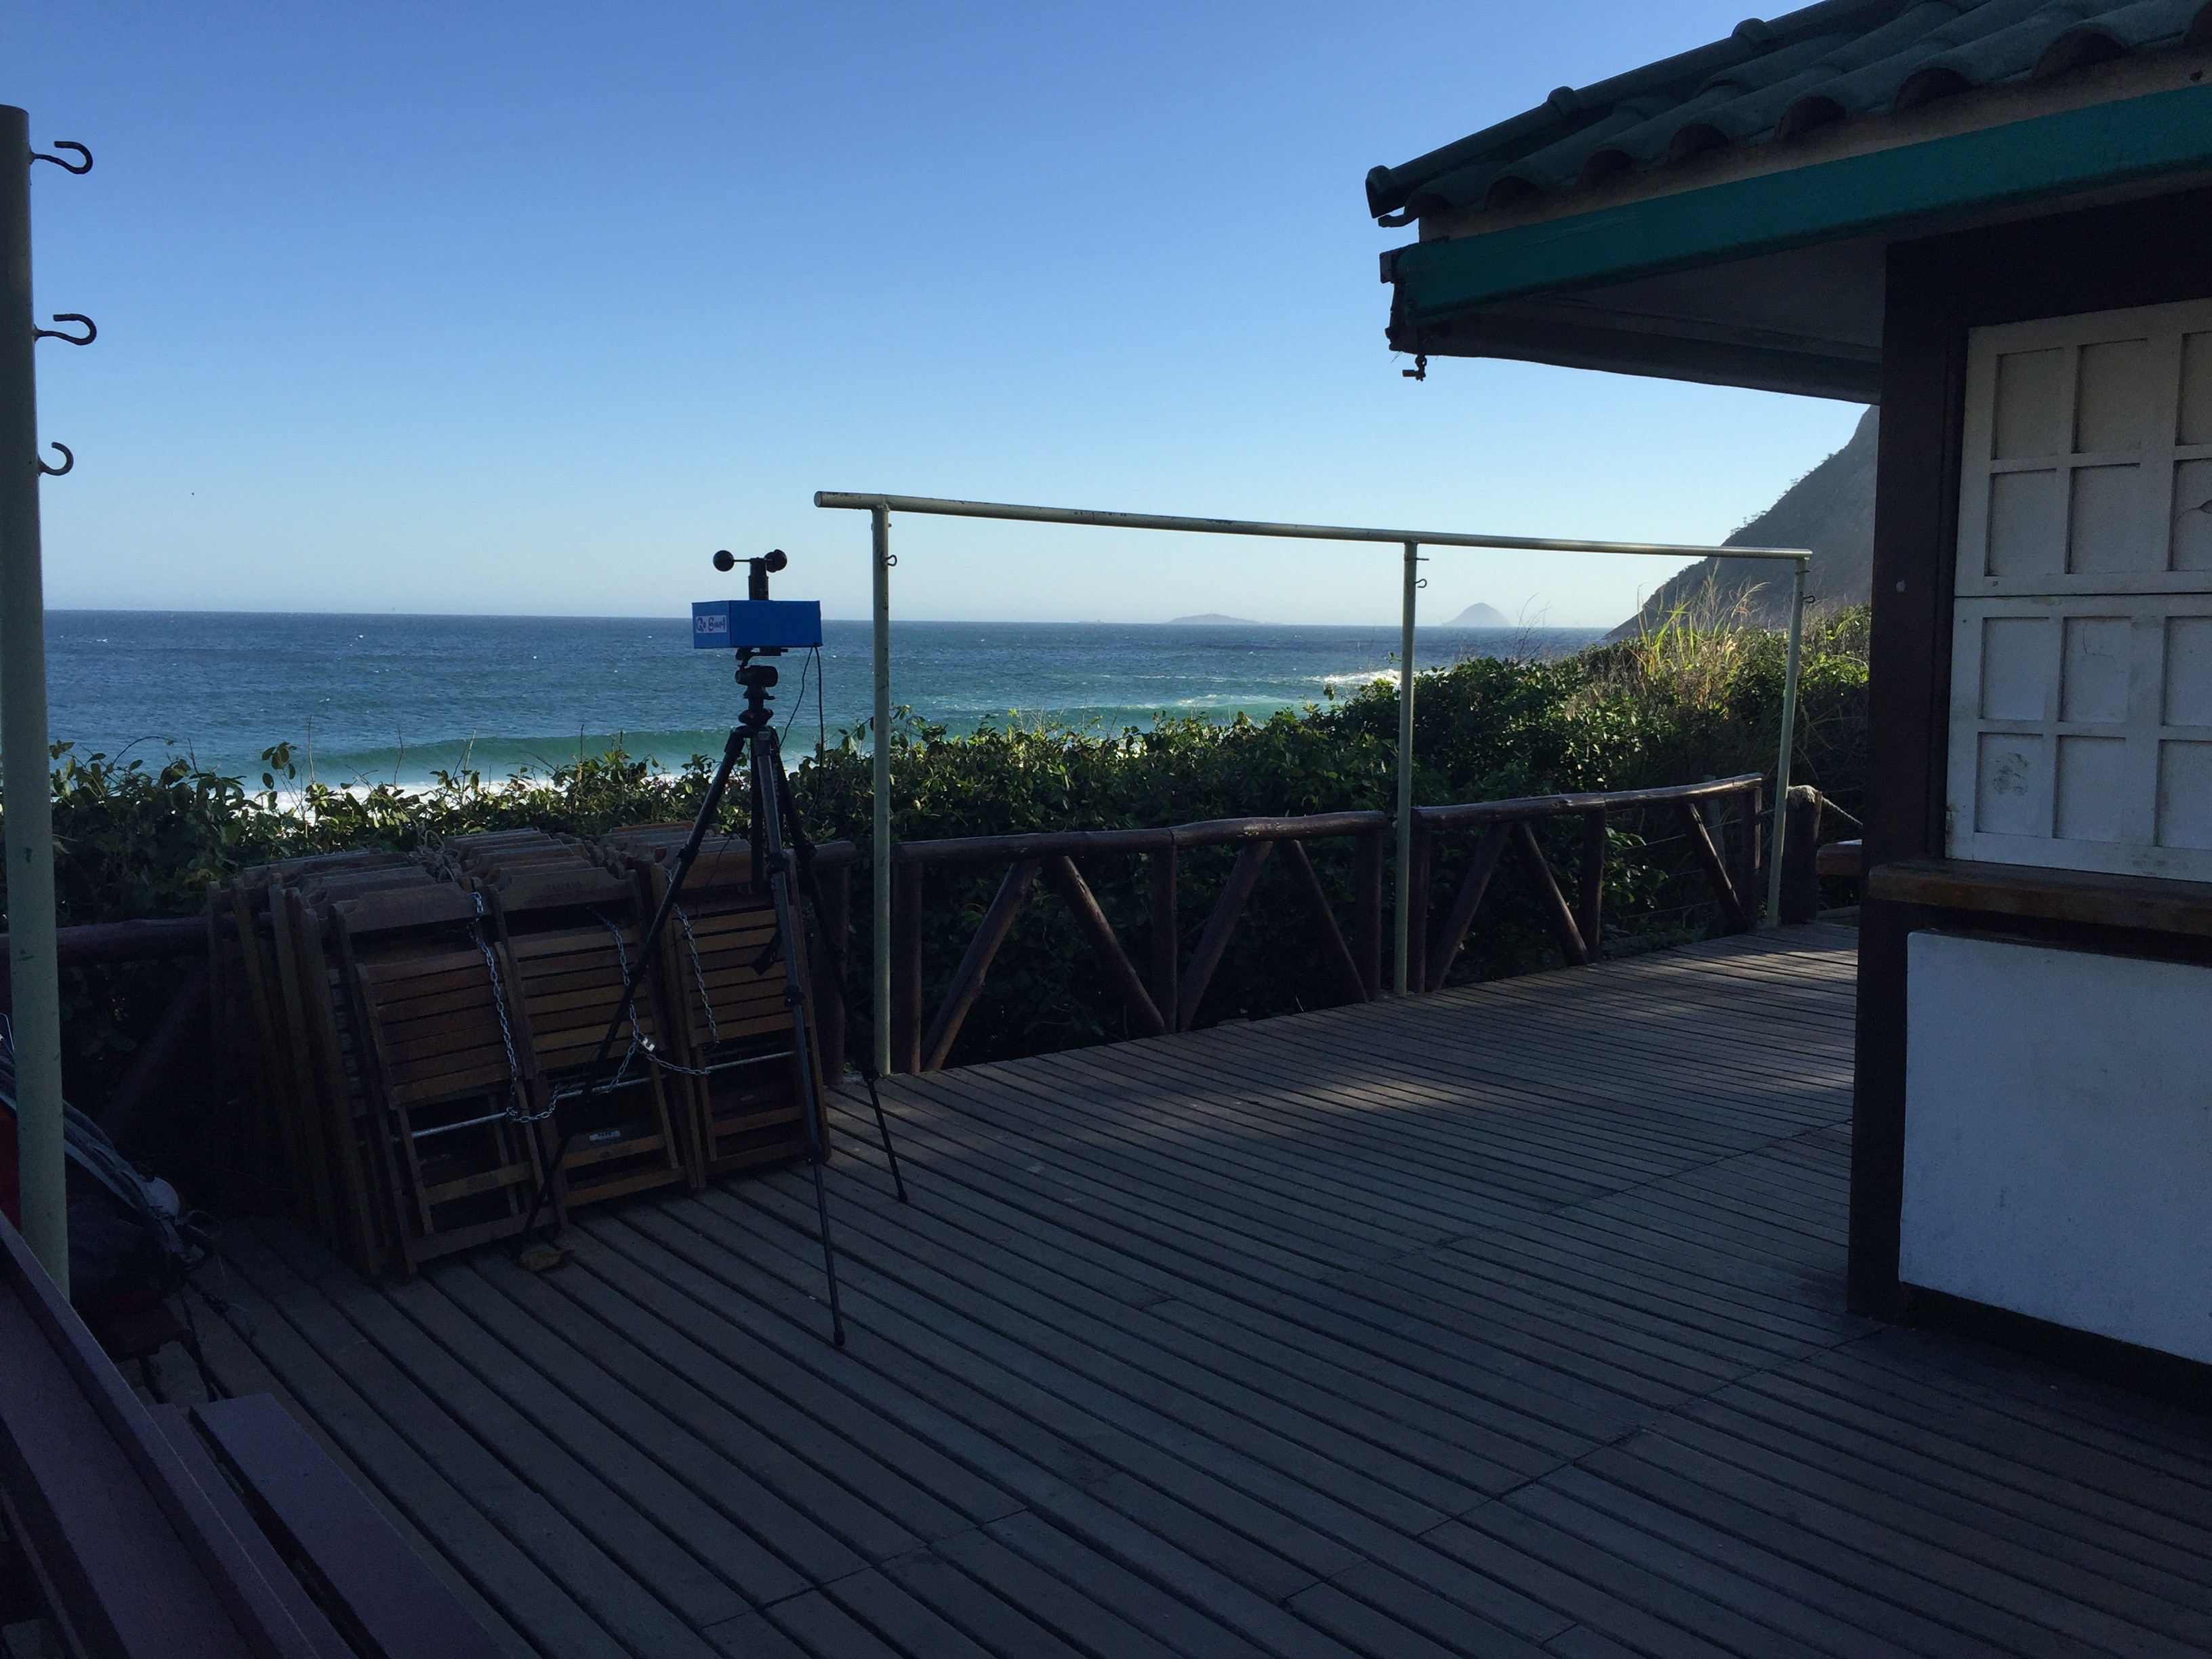
\includegraphics[height=.25\textheight,keepaspectratio]{IMG_0914.jpg}}
    \qquad
    \subfloat[\small{Aparato de \textit{hardware} posicionado.}]{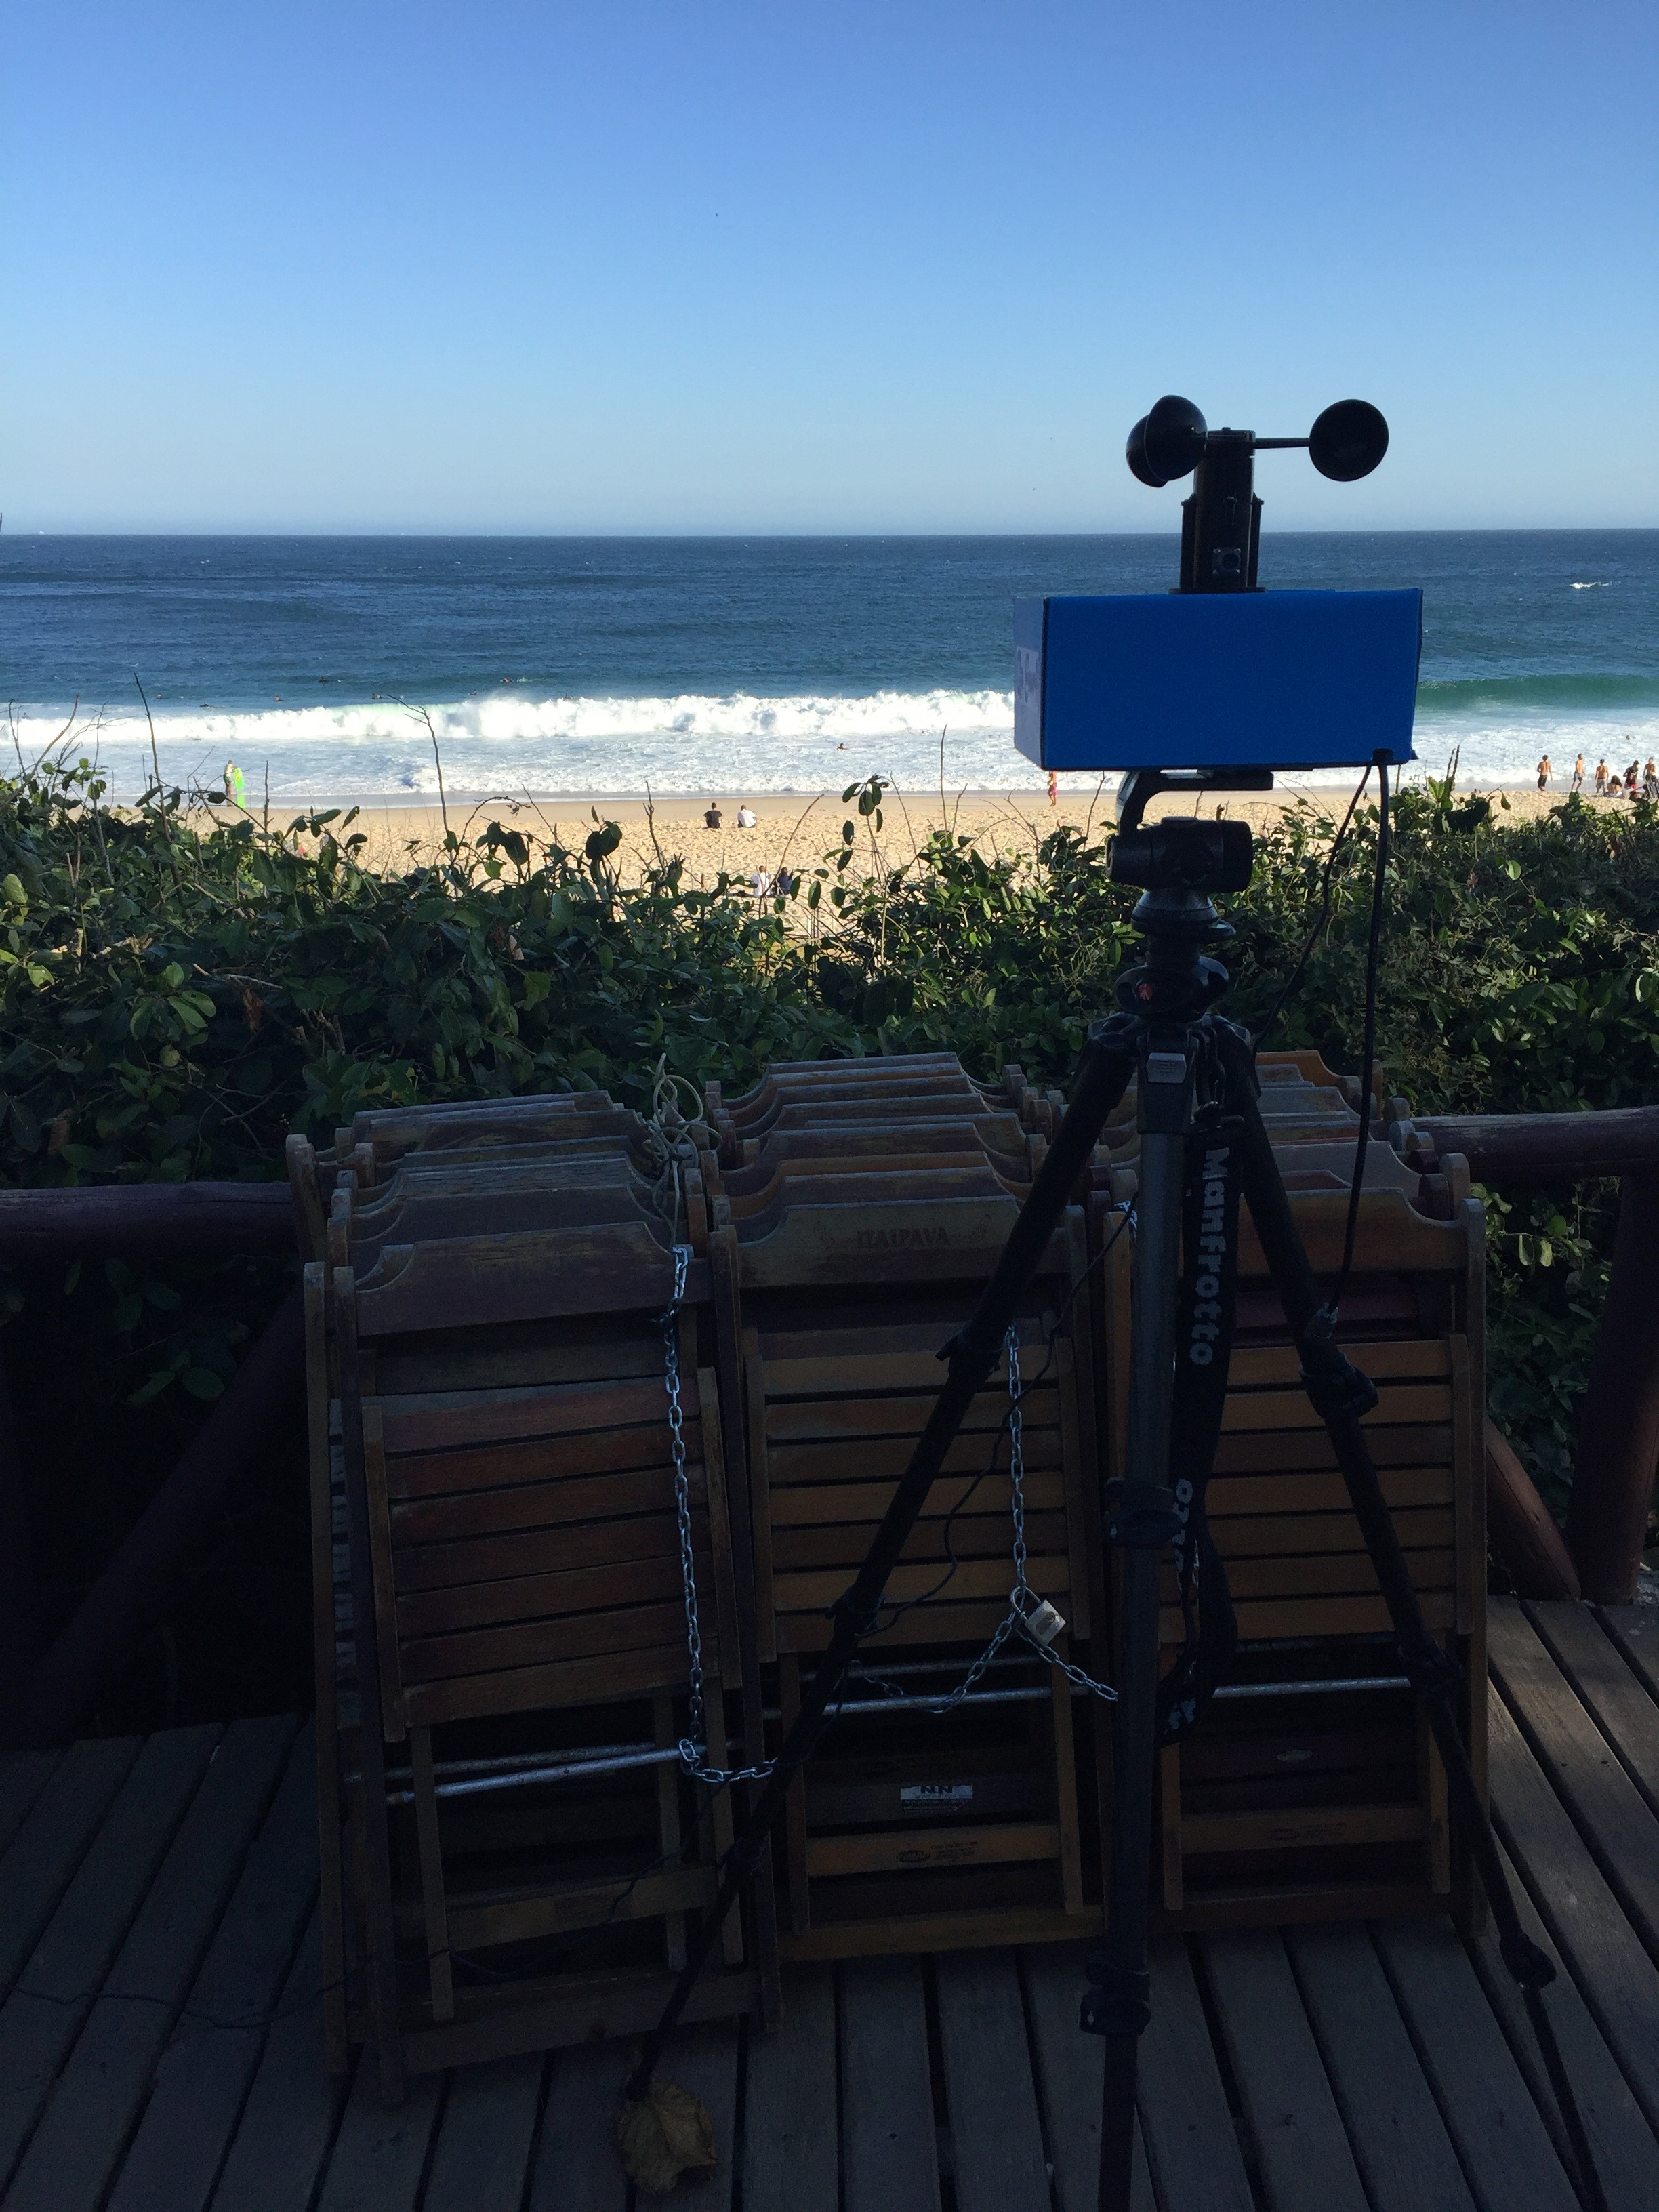
\includegraphics[height=.25\textheight,keepaspectratio]{IMG_0913.jpg}}
    \caption[\small{Local na praia de Itacoatiara onde os v�deos foram capturados.}]{\small{Local na praia de Itacoatiara onde os v�deos foram capturados.}}
    \label{FigDataLocation}
\end{figure}

\paragraph{}Foram analisados 18 v�deos, contemplando quatro dias distintos. Para cada v�deo as ondas foram analisadas automaticamente pelo algoritmo e manualmente pelo autor, a fim de verificar quantas ondas foram ou deixaram de ser identificadas, e verificar a precis�o da identifica��o do ponto m�nimo e m�ximo da onda. No total foram identificadas 200 ondas manualmente e 225 ondas pelo algoritmo, o que representa uma taxa de acerto de 88\%. Entretanto, como ser� mostrado, a taxa de acerto de cada v�deo individual pode variar. Os dados obtidos foram apresentados nas tabelas \ref{Tab20170704}, \ref{Tab20170708}, \ref{Tab20170709}, \ref{Tab20170807_1} e \ref{Tab20170807_2}, referentes aos respectivos dias: 04/07/2017, 08/07/2017, 09/07/2017 e 07/08/2017. O dia 04/07/2017 apresentava c�u nublado e mar revolto, sem a presen�a de banhistas na areia ou mar. J� os dias 08/07/2017 e 09/07/2017 apresentavam c�u aberto e mar calmo, sendo algumas s�ries com ondas um pouco maiores. Pode-se observar a presen�a de pessoas na areia e surfistas no mar. O dia 07/08/2017 apresentada c�u aberto e mar calmo, por�m mais agitado que os dias 08/07/2017 e 09/07/2017. N�o h� muitos banhistas, mas � poss�vel notar uma boa quantidade de surfistas. 

\paragraph{}Para facilitar a an�lise manual dos v�deos foi desenvolvido um programa de inspe��o de v�deos de praia denominado WaveInspector. Este programa permite ao usu�rio assistir um v�deo gravado de forma acelerada, pausar e retomar a execu��o do v�deo, e, com o v�deo pausado, selecionar com o mouse os pontos m�ximos e m�nimos de uma onda observada na imagem. Uma vez escolhidos os dois pontos, � poss�vel salvar ou descartar os dados selecionados. No final da execu��o do v�deo um arquivo texto � gerado contendo os pontos m�ximos e m�nimos de cada onda e o n�mero do \textit{frame} em que a medi��o foi realizada. Salva-se tamb�m o \textit{frame} em si com uma linha vertical indicando o centro da imagem. A figura \ref{FigSegmentataionFixedObject}a foi gerada utilizando o programa WaveInspector.

\begin{table}[h]
    \subfloat[\small{Dados de um v�deo com 1:25 minutos de dura��o gravado com \textit{smartphone}.}]{
	   \begin{tabular}{|l|l|l|}
\hline
Par�metros & Valores (manuais) & Valores (algoritmo) \\ \hline
N�mero de Ondas Encontradas & 7 & 10 \\ \hline
Altura m�dia das Ondas (pixels) & 20.8571 & 16.3 \\ \hline
Desvio Padr�o (pixels) & 3.79581 & 5.67539 \\ \hline
Altura m�dia das Ondas (metros) & 0.885888 & 0.720212 \\ \hline
Desvio Padr�o (metros$^{2}$) & 0.182062 & 0.240695 \\ \hline
\end{tabular}

    }
    \qquad
    \subfloat[\small{Dados de um v�deo com 1:01 minutos de dura��o gravado com \textit{smartphone}.}]{
        \begin{tabular}{|l|l|l|}
\hline
Par�metros & Valores (manuais) & Valores (algoritmo) \\ \hline
N�mero de Ondas Encontradas & 6 & 5 \\ \hline
Altura m�dia das Ondas (pixels) & 20.1667 & 19.8 \\ \hline
Desvio Padr�o (pixels) & 4.01732 & 2.22711 \\ \hline
Altura m�dia das Ondas (metros) & 0.794227 & 0.792542 \\ \hline
Desvio Padr�o (metros$^{2}$) & 0.145238 & 0.0917604 \\ \hline
\end{tabular}

    }
    \qquad
    \subfloat[\small{Dados de um v�deo com 1:33 minutos de dura��o gravado com \textit{smartphone}.}]{
        \begin{tabular}{|l|l|l|}
\hline
Par�metros & Valores (manuais) & Valores (algoritmo) \\ \hline
N�mero de Ondas Encontradas & 5 & 8 \\ \hline
Altura m�dia das Ondas (pixels) & 25.4 & 22 \\ \hline
Desvio Padr�o (pixels) & 5.2 & 9.86154 \\ \hline
Altura m�dia das Ondas (metros) & 1.03689 & 0.866055 \\ \hline
Desvio Padr�o (metros$^{2}$) & 0.226292 & 0.391268 \\ \hline
\end{tabular}

    }
    \qquad
    \subfloat[\small{Dados de um v�deo com 2:51 minutos de dura��o gravado com \textit{smartphone}.}]{
        \begin{tabular}{|l|l|l|}
\hline
Par�metros & Valores (manuais) & Valores (algoritmo) \\ \hline
N�mero de Ondas Encontradas & 11 & 21 \\ \hline
Altura m�dia das Ondas (pixels) & 26.4545 & 25.4286 \\ \hline
Desvio Padr�o (pixels) & 4.86852 & 14.7538 \\ \hline
Altura m�dia das Ondas (metros) & 2.36692 & 1.89405 \\ \hline
Desvio Padr�o (metros$^{2}$) & 0.447306 & 1.12171 \\ \hline
\end{tabular}

    }
	\caption[\small{Dados dos v�deos gravados no dia 04/07/2017}]{\small{Dados dos v�deos gravados no dia 04/07/2017}}
	\label{Tab20170704}
\end{table}

\begin{table}[h]
	\centering
    \subfloat[\small{Dados de um v�deo com 1:58 minutos de dura��o gravado com \textit{smartphone}.}]{
	   \begin{tabular}{|l|l|l|}
\hline
Par�metros & Valores (manuais) & Valores (algoritmo) \\ \hline
N�mero de Ondas Encontradas & 10 & 10 \\ \hline
Altura m�dia das Ondas (pixels) & 14.9 & 19.6 \\ \hline
Desvio Padr�o (pixels) & 1.64012 & 5.4626 \\ \hline
Altura m�dia das Ondas (metros) & 1.04373 & 1.22885 \\ \hline
Desvio Padr�o (metros$^{2}$) & 0.210381 & 0.364861 \\ \hline
\end{tabular}

    }
    \qquad
    \subfloat[\small{Dados de um v�deo com 2:58 minutos de dura��o gravado com \textit{smartphone}.}]{
        \begin{tabular}{|l|l|l|}
\hline
Par�metros & Valores (manuais) & Valores (algoritmo) \\ \hline
N�mero de Ondas Encontradas & 13 & 9 \\ \hline
Altura m�dia das Ondas (pixels) & 16.0769 & 17.6667 \\ \hline
Desvio Padr�o (pixels) & 4.56511 & 5.7735 \\ \hline
Altura m�dia das Ondas (metros) & 1.18953 & 1.32342 \\ \hline
Desvio Padr�o (metros$^{2}$) & 0.323158 & 0.424932 \\ \hline
\end{tabular}
    
    }
	\caption[\small{Dados dos v�deos gravados no dia 08/07/2017}]{\small{Dados dos v�deos gravados no dia 08/07/2017}}
	\label{Tab20170708}
\end{table}

\begin{table}[h]
	\centering
    \subfloat[\small{Dados de um v�deo com 2:13 minutos de dura��o gravado com \textit{smartphone}.}]{
	   \begin{tabular}{|l|l|l|}
\hline
Par�metros & Valores (manuais) & Valores (algoritmo) \\ \hline
N�mero de Ondas Encontradas & 10 & 11 \\ \hline
Altura m�dia das Ondas (pixels) & 16.2 & 19.1818 \\ \hline
Desvio Padr�o (pixels) & 3.96989 & 8.40799 \\ \hline
Altura m�dia das Ondas (metros) & 1.13346 & 1.33869 \\ \hline
Desvio Padr�o (metros$^{2}$) & 0.260627 & 0.569869 \\ \hline
\end{tabular}

    }
    \qquad
    \subfloat[\small{Dados de um v�deo com 1:45 minutos de dura��o gravado com \textit{smartphone}.}]{
        \begin{tabular}{|l|l|l|}
\hline
Par�metros & Valores (manuais) & Valores (algoritmo) \\ \hline
N�mero de Ondas Encontradas & 8 & 7 \\ \hline
Altura m�dia das Ondas (pixels) & 16.25 & 26.5714 \\ \hline
Desvio Padr�o (pixels) & 4.94343 & 11.425 \\ \hline
Altura m�dia das Ondas (metros) & 0.529188 & 0.83094 \\ \hline
Desvio Padr�o (metros$^{2}$) & 0.174855 & 0.366174 \\ \hline
\end{tabular}

    }
    \qquad
    \subfloat[\small{Dados de um v�deo com 8:37 minutos de dura��o gravado com \textit{smartphone}.}]{
        \begin{tabular}{|l|l|l|}
\hline
Par�metros & Valores (manuais) & Valores (algoritmo) \\ \hline
N�mero de Ondas Encontradas & 31 & 34 \\ \hline
Altura m�dia das Ondas (pixels) & 19.7097 & 25.1765 \\ \hline
Desvio Padr�o (pixels) & 4.03368 & 10.6949 \\ \hline
Altura m�dia das Ondas (metros) & 0.759227 & 0.936588 \\ \hline
Desvio Padr�o (metros$^{2}$) & 0.183345 & 0.401502 \\ \hline
\end{tabular}

    }
	\caption[\small{Dados dos v�deos gravados no dia 09/07/2017}]{\small{Dados dos v�deos gravados no dia 09/07/2017}}
	\label{Tab20170709}
\end{table}

\begin{table}[h]
    \centering
    \subfloat[\small{Dados de um v�deo 0:57 segundos de dura��o gravado com o aparato de \textit{hardware}.}]{
        \begin{tabular}{|l|l|l|}
\hline
Par�metros & Valores (manuais) & Valores (algoritmo) \\ \hline
N�mero de Ondas Encontradas & 5 & 5 \\ \hline
Altura m�dia das Ondas (pixels) & 22 & 19 \\ \hline
Desvio Padr�o (pixels) & 3.57771 & 6.63325 \\ \hline
Altura m�dia das Ondas (metros) & 0.728184 & 0.629375 \\ \hline
Desvio Padr�o (metros$^{2}$) & 0.142697 & 0.218883 \\ \hline
\end{tabular}

    }
    \qquad
    \subfloat[\small{Dados de um v�deo 0:58 segundos de dura��o gravado com o aparato de \textit{hardware}.}]{
        \begin{tabular}{|l|l|l|}
\hline
Par�metros & Valores (manuais) & Valores (algoritmo) \\ \hline
N�mero de Ondas Encontradas & 7 & 7 \\ \hline
Altura m�dia das Ondas (pixels) & 22.2857 & 19 \\ \hline
Desvio Padr�o (pixels) & 4.29998 & 6.98979 \\ \hline
Altura m�dia das Ondas (metros) & 0.755147 & 0.638611 \\ \hline
Desvio Padr�o (metros$^{2}$) & 0.156599 & 0.239838 \\ \hline
\end{tabular}

    }
    \qquad
    \subfloat[\small{Dados de um v�deo 1:43 minutos de dura��o gravado com o aparato de \textit{hardware}.}]{
        \begin{tabular}{|l|l|l|}
\hline
Par�metros & Valores (manuais) & Valores (algoritmo) \\ \hline
N�mero de Ondas Encontradas & 7 & 8 \\ \hline
Altura m�dia das Ondas (pixels) & 17 & 20.75 \\ \hline
Desvio Padr�o (pixels) & 4.8107 & 7.42883 \\ \hline
Altura m�dia das Ondas (metros) & 0.570377 & 0.672538 \\ \hline
Desvio Padr�o (metros$^{2}$) & 0.169628 & 0.244401 \\ \hline
\end{tabular}

    }
    \qquad
    \subfloat[\small{Dados de um v�deo 4:50 minutos de dura��o gravado com o aparato de \textit{hardware}.}]{
        \begin{tabular}{|l|l|l|}
\hline
Par�metros & Valores (manuais) & Valores (algoritmo) \\ \hline
N�mero de Ondas Encontradas & 27 & 26 \\ \hline
Altura m�dia das Ondas (pixels) & 16.2222 & 19.6538 \\ \hline
Desvio Padr�o (pixels) & 5.23049 & 8.23661 \\ \hline
Altura m�dia das Ondas (metros) & 0.551704 & 0.645299 \\ \hline
Desvio Padr�o (metros$^{2}$) & 0.192213 & 0.271287 \\ \hline
\end{tabular}

    }
    \caption[\small{Dados dos v�deos gravados no dia 07/08/2017}]{\small{Dados dos v�deos gravados no dia 07/08/2017}}
    \label{Tab20170807_1}
\end{table}

\begin{table}[h]
    \centering
    \subfloat[\small{Dados de um v�deo 1:57 minutos de dura��o gravado com o aparato de \textit{hardware}.}]{
        \begin{tabular}{|l|l|l|}
\hline
Par�metros & Valores (manuais) & Valores (algoritmo) \\ \hline
N�mero de Ondas Encontradas & 13 & 13 \\ \hline
Altura m�dia das Ondas (pixels) & 16.6154 & 22.6923 \\ \hline
Desvio Padr�o (pixels) & 4.68284 & 6.85436 \\ \hline
Altura m�dia das Ondas (metros) & 0.599012 & 0.776419 \\ \hline
Desvio Padr�o (metros$^{2}$) & 0.175766 & 0.230962 \\ \hline
\end{tabular}

    }
    \qquad
    \subfloat[\small{Dados de um v�deo 4:54 minutos de dura��o gravado com o aparato de \textit{hardware}.}]{
        \begin{tabular}{|l|l|l|}
\hline
Par�metros & Valores (manuais) & Valores (algoritmo) \\ \hline
N�mero de Ondas Encontradas & 22 & 32 \\ \hline
Altura m�dia das Ondas (pixels) & 16 & 20.5312 \\ \hline
Desvio Padr�o (pixels) & 4.27466 & 9.02768 \\ \hline
Altura m�dia das Ondas (metros) & 0.528549 & 0.629375 \\ \hline
Desvio Padr�o (metros$^{2}$) & 0.1546 & 0.282701 \\ \hline
\end{tabular}

    }
    \qquad
    \subfloat[\small{Dados de um v�deo 1:57 minutos de dura��o gravado com o aparato de \textit{hardware}.}]{
        \begin{tabular}{|l|l|l|}
\hline
Par�metros & Valores (manuais) & Valores (algoritmo) \\ \hline
N�mero de Ondas Encontradas & 10 & 10 \\ \hline
Altura m�dia das Ondas (pixels) & 15.5 & 17.1 \\ \hline
Desvio Padr�o (pixels) & 4.00625 & 10.4159 \\ \hline
Altura m�dia das Ondas (metros) & 0.526535 & 0.519233 \\ \hline
Desvio Padr�o (metros$^{2}$) & 0.148273 & 0.316641 \\ \hline
\end{tabular}

    }
    \caption[\small{Dados dos v�deos gravados no dia 07/08/2017}]{\small{Dados dos v�deos gravados no dia 07/08/2017}}
    \label{Tab20170807_2}
\end{table}

\begin{table}[h]
    \centering
    \subfloat[\small{Dados de um v�deo 0:45 segundos de dura��o gravado com \textit{smartphone}.}]{
        \begin{tabular}{|l|l|l|}
\hline
Par�metros & Valores (manuais) & Valores (algoritmo) \\ \hline
N�mero de Ondas Encontradas & 4 & 4 \\ \hline
Altura m�dia das Ondas (pixels) & 15.5 & 17.25 \\ \hline
Desvio Padr�o (pixels) & 4.15331 & 7.01338 \\ \hline
Altura m�dia das Ondas (metros) & 0.860654 & 0.953337 \\ \hline
Desvio Padr�o (metros$^{2}$) & 0.314605 & 0.392706 \\ \hline
\end{tabular}

    }
    \qquad
    \subfloat[\small{Dados de um v�deo 0:38 segundos de dura��o gravado com \textit{smartphone}.}]{
        \begin{tabular}{|l|l|l|}
\hline
Par�metros & Valores (manuais) & Valores (algoritmo) \\ \hline
N�mero de Ondas Encontradas & 4 & 5 \\ \hline
Altura m�dia das Ondas (pixels) & 18.5 & 17.8 \\ \hline
Desvio Padr�o (pixels) & 5.31507 & 3.18748 \\ \hline
Altura m�dia das Ondas (metros) & 1.04531 & 0.995072 \\ \hline
Desvio Padr�o (metros$^{2}$) & 0.318676 & 0.163918 \\ \hline
\end{tabular}

    }
\end{table}

\paragraph{}Alguns fatores podem interferir no algoritmo de estima��o de altura das ondas. Dentre estes fatores, pode-se classific�-los em duas categorias: problemas impeditivos e n�o impeditivos. Os problemas impeditivos impossibilitam completamente a identifica��o das regi�o de espuma do mar, e em geral possuem duas causas: baixa ilumina��o e interfer�ncia fixa de banhistas na areia. O problema da baixa ilumina��o foi discutido na se��o \ref{sec:segmentation_border_detection} e ilustrado pela figura \ref{FigThresholdFail}. J� a interfer�ncia de banhistas fixos ocorre quando alguma pessoa ou objeto est� posicionado sobre a coluna central de cada \textit{frame} do v�deo como na imagem \ref{FigSegmentataionFixedObject}. Esta pessoa ou objeto se traduz no \textit{timestack} como uma linha escura cont�nua. Esta linha divide a regi�o de espuma encontrada, formando duas regi�es de alta intensidade na imagem binarizada pela etapa de \textit{thresholding}. Dependendo da posi��o vertical onde a regi�o � dividida a regi�o de espuma pode n�o ser a maior regi�o segmentada pela imagem, fazendo com que a etapa de segmenta��o selecione a regi�o errada (por exemplo, selecione a faixa de areia ao inv�s de selecionar a regi�o de espuma). 

\begin{figure}[h]
    \centering
    \subfloat[\small{Frame do v�deo com um objeto fixo sobre a coluna central.}]{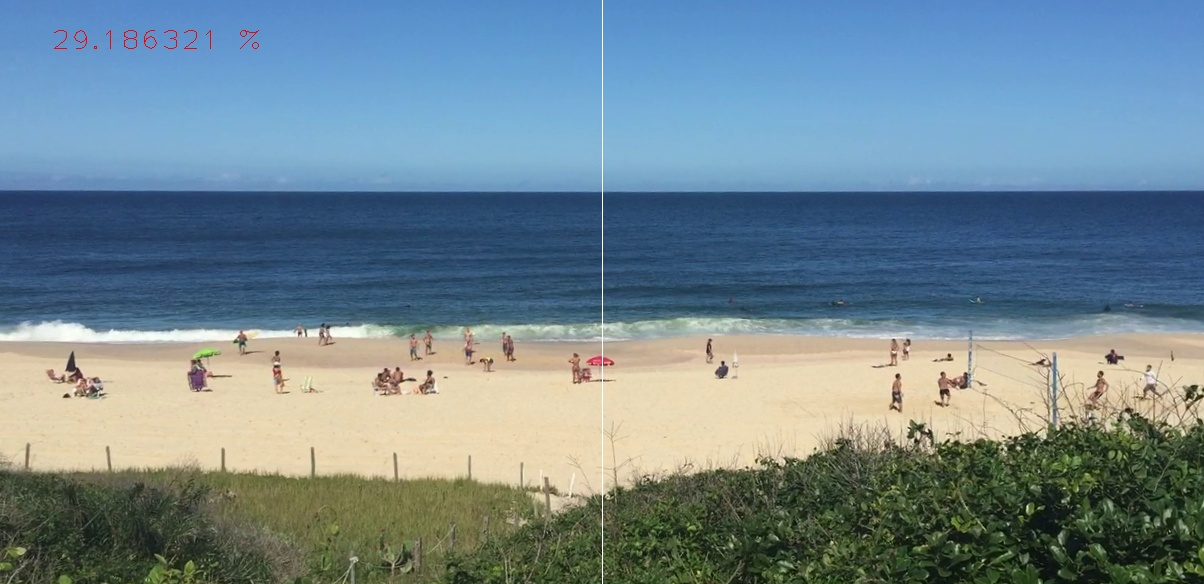
\includegraphics[width=.9\textwidth,keepaspectratio]{frame_object_middle.jpg}}
    \qquad
    \subfloat[\small{A linha escura na areia � resultado do objeto fixo no centro do v�deo.}]{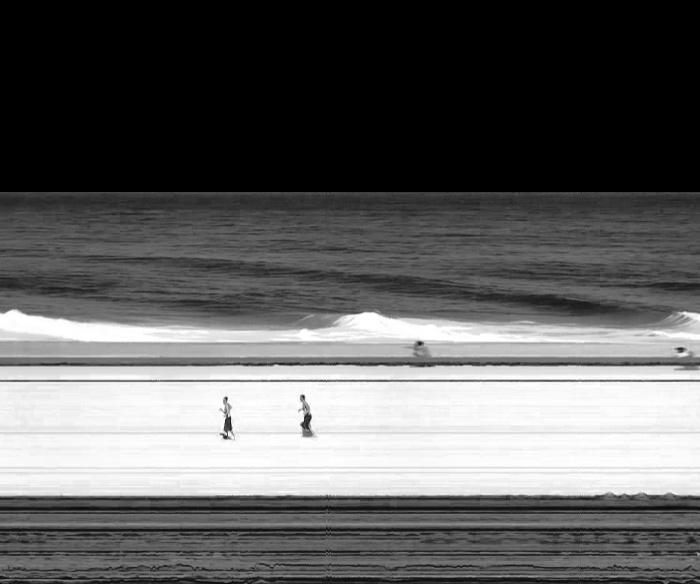
\includegraphics[width=.45\linewidth,keepaspectratio]{timestack_fixed_object_fail.png}}
    \qquad
    \subfloat[\small{Regi�o de espuma segmentada erroneamente.}]{
\includegraphics[width=.45\linewidth,keepaspectratio]{process_breakzone_fixed_object.png}}
    \caption[]{\small{Efeito resultante do guarda-sol fixo no centro de um v�deo.}}
    \label{FigSegmentataionFixedObject}
\end{figure}

\paragraph{}Os problemas n�o impeditivos est�o relacionados a erros na identifica��o de cada onda individualmente, como por exemplo detectar de um n�mero excessivo ou insuficiente de ondas em um v�deo, ou erros na identifica��o do ponto m�ximo ou m�nimo da onda. Esses erros n�o impedem que a imagem seja analisada, mas reduzem a confiabilidade do algoritmo. O problema de detec��o excessiva de n�mero excessivo de ondas ocorre principalmente em dias que o mar est� agitado. Nesta situa��o as ondas quebram com mais viol�ncia, resultando em um maior volume de espuma que pode ser identificado erroneamente como uma nova onda (Figura \ref{FigTimestackWaveNumberFail}). 

\begin{figure}[h]
    \centering
    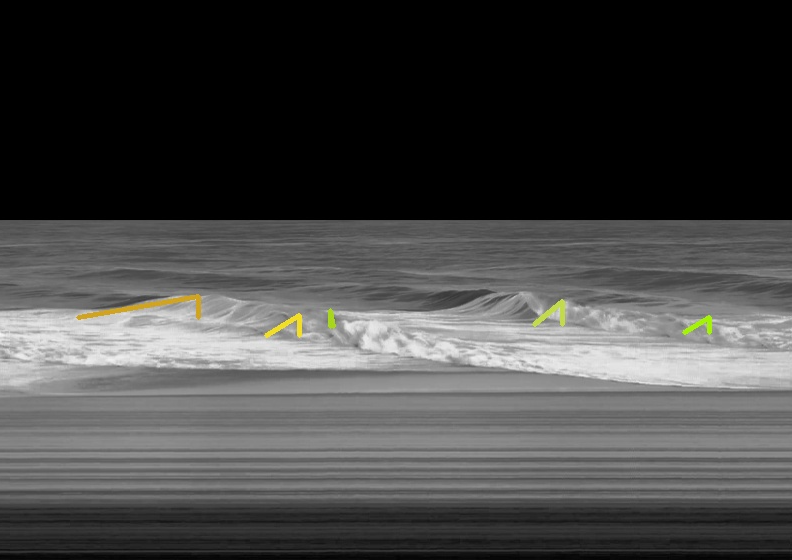
\includegraphics[width=.7\textwidth,keepaspectratio]{timestack_number_wave_fail.png}
    \caption[\small{\textit{Timestack} de um mar agitado. Tr�s foram identificadas al�m do esperado.}]{\small{\textit{Timestack} de um mar agitado. Tr�s ondas foram identificadas al�m do esperado.}}
    \label{FigTimestackWaveNumberFail}
\end{figure}

% \paragraph{}O caso de detec��o insuficiente de ondas � incomum, como pode-se observar nos dados exibidos anteriormente. \todo[inline]{finalizar este paragrafo.}

\begin{figure}[h]
    \centering

    \subfloat[\small{Onda detectada manualmente.}]{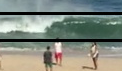
\includegraphics[width=.45\textwidth,keepaspectratio]{wave_people_manual.png}}
    \qquad
    \subfloat[\small{Onda detectada automaticamente.}]{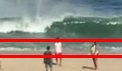
\includegraphics[width=.45\textwidth,keepaspectratio]{wave_people_automatic.png}}

    \caption[\small{Comparativo entre onda detectada manualmente e onda detectada automaticamente com interfer�ncia de pessoas na areia.}]{\small{Comparativo entre onda detectada manualmente e onda detectada automaticamente com interfer�ncia de pessoas na areia.}}
    \label{FigPeopleError}
\end{figure}

\paragraph{}Os erros na identifica��o dos pontos m�nimos e m�ximos em geral s�o causados por interfer�ncia externa, e influenciam na altura estimada da onda. A presen�a de pessoas se deslocando pr�ximos ao mar (Figura \ref{FigPeopleError}) � respons�vel por introduzir erros na identifica��o do ponto m�nimo de uma onda, fazendo com que pontos na areia sejam identificados como parte da regi�o de espuma. Outro fator que pode influenciar no ponto m�nimo da onda � o afastamento da onda da linha de arrebenta��o esperada. Em geral as ondas tendem a quebrar � uma mesma dist�ncia da praia, a linha de arrebenta��o esperada, onde ocorre um acumulo da espuma produzida pelas ondas. Algumas ondas, entretanto, podem arrebentar antes de atingirem a linha de arrebenta��o esperada, a uma dist�ncia maior da praia. Esta situa��o afeta a estima��o da altura da onda de duas maneiras:

\begin{enumerate}
    \item Ondas com dist�ncias diferentes da c�mera podem aparentar possuir a mesma altura em \textit{pixels}, quando na realidade possuem alturas diferentes. Al�m disso, Browne \textit{et al} \cite{Griffith11} demonstra que o erro associado aos par�metros da c�mera aumentam de acordo com a dist�ncia das ondas at� a c�mera.

    \item O ponto m�nimo da onda � identificado como o ponto m�nimo da linha de arrebenta��o imediatamente antes da quebra da onda. Quando uma onda quebra antes da linha de arrebenta��o, a sua base ser� erroneamente detectada como o ponto m�nimo da linha de arrebenta��o anterior. Este efeito � evid�nciado na figura \ref{FigBaseGap} e pode ocorrer quando h� um distanciamento temporal entre duas ondas. A se��o \ref{sec:wave_identification} apresenta uma forma de remediar este problema, mas que n�o resolve completamente o problema.
\end{enumerate}

\begin{figure}[h]
    \centering

    \subfloat[\small{Onda acima da linha de arrebenta��o. A base da onda n�o foi identificada corretamente.}]{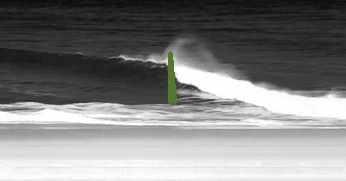
\includegraphics[height=.125\textheight,keepaspectratio]{wave_min_fail_gap.png}}
    \qquad
    \subfloat[\small{Onda acima da linha de arrebenta��o. A identifica��o da sua base foi corrigida.}]{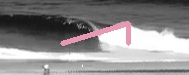
\includegraphics[height=.125\textheight,keepaspectratio]{wave_min_fail_gap_fixed.png}}

    \caption[\small{Efeito do afastamento da onda em rela��o a linha de arrebenta��o.}]{\small{Efeito do afastamento da onda em rela��o a linha de arrebenta��o.}}
    \label{FigBaseGap}
\end{figure}

\paragraph{}A a��o do vento \cite{Hwang2016} pode introduzir erros na identifica��o do ponto de m�ximo, causando um \textit{spray} da espuma do mar que pode ser erroneamente detectado como o ponto m�ximo da onda (Figura \ref{FigSprayError}).

\begin{figure}[h]
	\centering

	\subfloat[\small{Onda detectada manualmente.}]{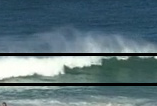
\includegraphics[width=.45\textwidth,keepaspectratio]{wave_spray_manual.png}}
    \qquad
	\subfloat[\small{Onda detectada automaticamente.}]{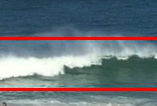
\includegraphics[width=.45\textwidth,keepaspectratio]{wave_spray_automatic.png}}

	\caption[\small{Comparativo entre onda detectada manualmente e onda detectada automaticamente com efeito de \textit{spray} de espuma.}]{\small{Comparativo entre onda detectada manualmente e onda detectada automaticamente com efeito de \textit{spray} de espuma.}}

	\label{FigSprayError}
\end{figure}

\paragraph{}Os dados apresentados nas tabelas \ref{Tab20170704}, \ref{Tab20170708} e \ref{Tab20170709} demonstram que apesar dos poss�veis erros relatados, a altura estimada m�dia das ondas est� dentro um limite satisfat�rio das ondas medidas manualmente, comprovando que o algoritmo proposto atende a proposta inicial deste projeto de gradua��o.

% ---------------------------------------------------------------
% Chapter 6 - Conclus�es
% ---------------------------------------------------------------
\chapter{Conclus�es}
\label{cap6}
\paragraph{}Neste trabalho foi implementado um novo m�todo de estima��o de alturas de ondas do mar utilizando t�cnicas de processamento de imagens. A biblioteca de processamento gr�fico OpenCV foi utilizada para facilitar a implementa��o do algoritmo e agilizar o desenvolvimento. Tamb�m foi apresentado um aparato de hardware utilizado para realizar a captura dos dados.

%Dificuldades
\paragraph{}As principais dificuldades deste projeto estavam relacionados a segmenta��o das ondas, a varia��o da ilumina��o sobre a imagem e a identifica��o da onda em si. A utiliza��o de \textit{timestacks} ao inv�s de processar os \textit{frames} individuais do v�deo se mostrou fundamental para facilitar a segmenta��o, pois reduziu drasticamente a quantidade de ru�do presente na imagem, facilitando a identifica��o do que � uma onda e o que � o restante do mar. O \textit{timestack} tamb�m foi uma pe�a importante para reduzir o volume de dados que � processado, da ordem de centenas de megabytes para dezenas de kilobytes. A varia��o da ilumina��o se mostrou um desafio, em alguns casos impossibilitando completamente a aplica��o do algoritmo, apesar da aplica��o da equaliza��o da imagem como tentativa de remediar o seu efeito. Por �ltimo a identifica��o da onda atrav�s da determina��o do seu ponto m�ximo e m�nimo apresentou dificuldades, sofrendo interfer�ncia de agentes externos e introduzindo assim erros na estima��o da altura da onda. Entretanto, os dados experimentais mostraram que apesar dos problemas conhecidos, as estimativas m�dias feitas pelo algoritmo est�o dentro dos valores esperados quando comparadas com medidas manuais para um mesmo conjunto de dados.

%Trabalhos futuros
\paragraph{}Como trabalho futuro planeja-se implementar a t�cnica de compatibiliza��o de histograma (\textit{histogram matching}) como poss�vel solu��o para o problema de ilumina��o. Este m�todo tem como objetivo alterar a distribui��o de um histograma para algum formato desejado. A t�cnica utilizada neste projeto, equaliza��o de histograma, � um caso espec�fico da compatibiliza��o de histograma onde o formato desejado � uma linha horizontal.

\paragraph{}Outro trabalho futuro � a identifica��o e remo��o da faixa de areia da imagem, de forma an�loga a identifica��o e remo��o do c�u realizada no pr�-processamento. Entretanto, a faixa de areia � mais dif�cil de identificar que o c�u, por n�o possuir uma linha divis�ria bem definida como a linha do horizonte. A sua remo��o seria importante para minimizar a interfer�ncia de banhistas na imagem como discutido no Cap�tulo 5.

\paragraph{}Um terceiro trabalho futuro � alterar o m�todo de remo��o do c�u. Durante do desenvolvimento do trabalho percebeu-se que a faixa de \textit{pixels} pretos gerada pela remo��o do c�u interfere com o limiar calculado pelo m�todo de Otsu durante \textit{thresholding}, sendo uma poss�vel solu��o realizar um corte na imagem, eliminando completamente os \textit{pixels} do c�u e reduzindo assim a altura da imagem. Entretanto, o menor valor de altura altera os valores encontrados para o ponto m�nimo e m�ximo das ondas, impactanto a convers�o de altura em \textit{pixels} para a altura real. Para corrigir este problema � necess�rio encontrar uma forma de converter os pontos encontrados na imagem reduzida para o seu equivalente em uma imagem com a altura original do v�deo capturado.

\paragraph{}Um �ltimo poss�vel trabalho futuro � a pesquisa e o desenvolvimento de um \textit{hardware} aut�nomo, resistente �s condi��es clim�ticas de uma praia. O \textit{hardware} utilizado para a aquisi��o dos dados deste projeto serviu apenas em car�ter provis�rio, sendo exposto apenas temporariamente ao ambiente da praia. Um \textit{hardware} permanente deve ser capaz de suportar a exposi��o a maresia, sol e chuva sem prejudicar o seu funcionamento. Al�m disso, ele n�o deve depender de fontes de energia externas, operando preferencialmente com energia solar e baterias.

% ---------------------------------------------------------------
% Bibliografia
% ---------------------------------------------------------------
\normalsize
\cleardoublepage
\addcontentsline{toc}{chapter}{Bibliografia}
\bibliographystyle{coppe}
\bibliography{biblio}

% ---------------------------------------------------------------
% Ap�ndices 
% ---------------------------------------------------------------
   \appendix
   % ---------------------------------------------------------------
   % Ap�ndice A
   % ---------------------------------------------------------------
   \chapter{Ferramenta WaveInspector}
   \label{ApendiceA}
   \paragraph{}Elemento que consiste em um texto ou documento elaborado pelo autor, com o intuito de complementar sua argumenta��o, sem preju�zo do trabalho. S�o identificados por letras mai�sculas consecutivas e pelos respectivos t�tulos.
   % ---------------------------------------------------------------
   % Ap�ndice B
   % ---------------------------------------------------------------
   \chapter{Encaderna��o do Projeto de Gradua��o}
   \label{ApendiceB}
   \begin{figure}
\begin{center}
\parbox[htb]{13.0cm}
  {
  \begin{center}
  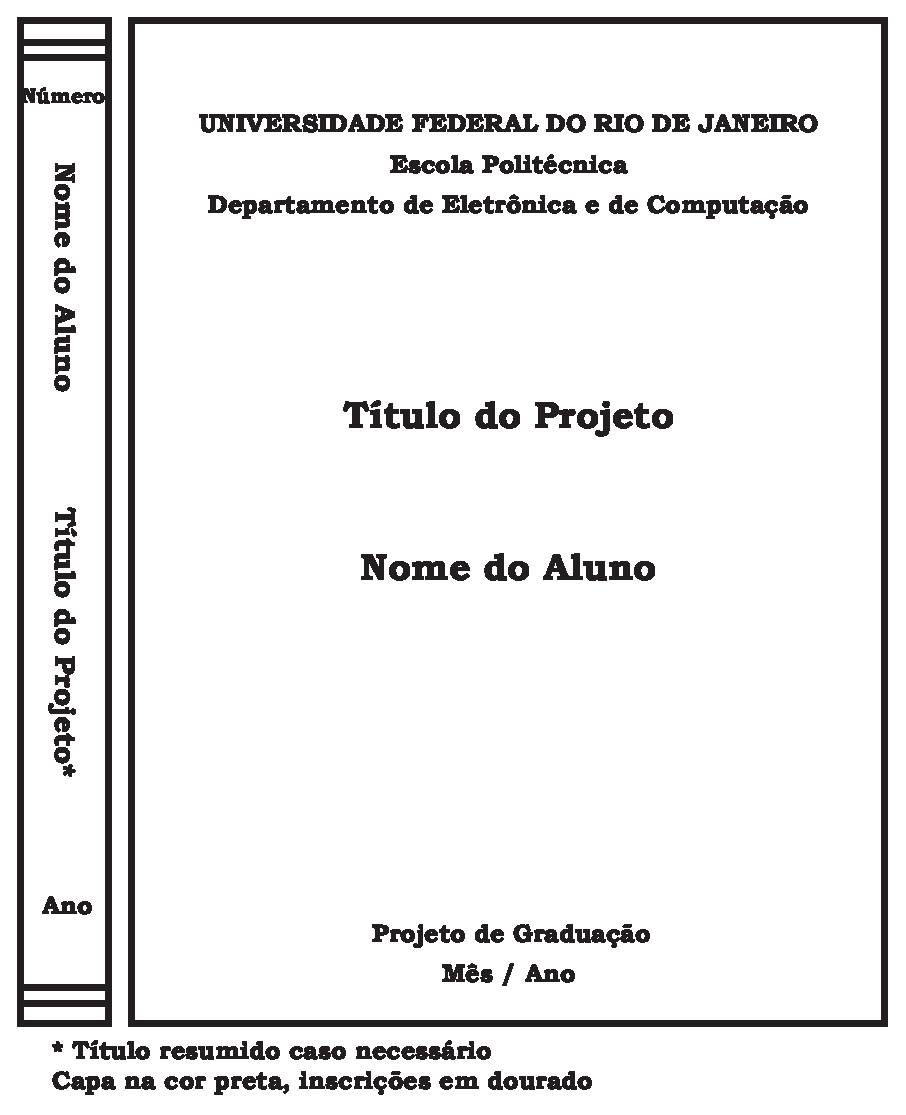
\includegraphics[scale=1.0]{Capa_do_Projeto_Final.eps}
  \caption[\small{Encaderna��o do projeto de gradua��o.}]{\label{FigPFC} \small{Encaderna��o do projeto de gradua��o.}}
  \end{center}
  }
\end{center}
\end{figure}
   % ---------------------------------------------------------------
   % Ap�ndice C
   % ---------------------------------------------------------------
   \chapter{O que � um anexo}
   \label{ApendiceC}
   \paragraph{}Documenta��o n�o elaborada pelo autor, ou elaborada pelo autor mas constituindo parte de outro projeto.   

\backmatter

\end{document}
